\documentclass[12pt,masters]{style/ucbthesis}
%\includeonly{include/method}
\usepackage{style/basic}
\usepackage{style/glossary}
%\usepackage{style/my_format}
\usepackage{style/commands}
\usepackage{style/matlab}
\usepackage[textsize=tiny]{todonotes}
\def\wdt{\gls{wdt}}

\newacronym{bwr}{BWR}{Boiling Water Reactor}
\newacronym{cdf}{CDF}{cumulative density function}
\newacronym{cfe}{CFE}{collision flux estimator}
\newacronym{fom}{FOM}{figure of merit}
\newacronym{inl}{INL}{Idaho National Lab}
\newacronym{pdf}{PDF}{probability density function}
\newacronym{tle}{TLE}{track-length estimator}
\newacronym{treat}{TREAT}{Transient Reactor Test Facility}
\newacronym{wdt}{WDT}{weighted delta-tracking}




\begin{document}
\listoftodos
\newpage
\title{Weighted Delta-Tracking with Scattering implemented in the
  Serpent 2 Monte Carlo Code}
\author{J.S. Rehak}
\degreesemester{Spring}
\degreeyear{2017}
\degree{Masters of Science}
\chair{Professor Rachael Slaybaugh}
\othermembers{Professor Massimiliano Fratoni \\
  Professor Leslie Kerby}
\numberofmembers{3}
\field{Nuclear Engineering}
\campus{Berkeley}

%% ==== OPENING ====================

\maketitle

\approvalpage
\copyrightpage

%% Abstract
%% (This file is included by thesis.tex; you do not latex it by itself.)

\begin{abstract}

% The text of the abstract goes here.  If you need to use a \section
% command you will need to use \section*, \subsection*, etc. so that
% you don't get any numbering.  You probably won't be using any of
% these commands in the abstract anyway.

Invasive brag; forbearance.

\end{abstract}


%% ===== FRONT MATTER ====================
\begin{frontmatter}

%% Dedication
%\begin{dedication}
\null\vfil
\begin{center}
Dedication
\end{center}
\vfil\null
\end{dedication}

\tableofcontents
\clearpage
\listoffigures
\clearpage
\listoftables

%% Acknowledgments
%\begin{acknowledgements}
Acknowledgments
\end{acknowledgements}

\end{frontmatter}

\pagestyle{headings}

%% ===== MAIN BODY ====================


\chapter{Introduction}
\label{sec:intro}

This is the introduction!

\chapter{Background}
\label{chap:background}

Monte Carlo codes are vital tools in a diverse number of fields. Based
in simple random number generators, these tools harness the power of
statistics to predict and describe a wide variety of behaviors. In
nuclear engineering, there is a long history of Monte Carlo methods
used to simulate neutral particle propagation. These methods enjoy a
wide variety of applications within the field, from fuel cell
development to full core analysis. A vital part of the simulation is
the propagation and interaction of neutral particles, neutrons. In
this chapter we will describe the history and mathematics of these
neutral particle propagation methods.

\section{The Monte Carlo Method}
\label{sec:monte_carlo}

The history of Monte Carlo methods begins with nuclear science and
engineering. Nicholas Metropolis and S. Ulam~\cite{metropolis1949} at
Los Alamos National Laboratory developed the method to support the
Manhattan Project. Today, Monte Carlo methods have found diverse
applications across the hard and social sciences. In nuclear
engineering, we still use Monte Carlo for its original purpose, the
propagation of neutral particles. Now, its use has expanded from
weapons research to assessing the viability and properties of nuclear
reactors.

When used for particle transport, the Monte Carlo method uses a random
number generator to simulate a particle's history. As the simulation
runs, various parameters are calculated and recorded. This will continue
for a finite number of histories, $N$, after which the mean value of
the parameters of interest are calculated:
\begin{equation*}
  \bar{x} = \frac{1}{N}\sum_{n=1}^Nx_n\:,
\end{equation*}
where $x_n$ is the value from the $n$-th history\cite{lewis1993}. The process
for sampling will be described in general here, and then extended to
particle propagation methods in Sec.~\ref{sec:propagation}.

As described by Lewis and Miller~\cite{lewis1993}, we first must
consider a random variable, $x$. We define the probability that $x$
will have a value between $a$ and $b$: $P\{a \leq x \leq b\}$. We
are interested in the probability that our random variable will have one
specific value. Therefore, we define the probability that our variable
will fall within a differential distance to a given value $x$ in the
limit that the differential distance goes to zero. This is the
\gls{pdf}, the probability that $x'$ will be between $x$ and $x +
\Delta x$:
\begin{equation}
  \label{eq:pdf_initial}
 f(x)\Delta x = \lim_{\Delta x \to 0}  P \{ x \leq x' \leq x + \Delta x \}\:.
\end{equation}
Integrating the \gls{pdf} gives the overall probability for the range:
\begin{equation}
\label{pdf}
  \int_a^bf(x)dx = P\{a \leq x \leq b\}\:.
\end{equation}
If we integrate the \gls{pdf} over the entire range of possible values
of $x$, it must equal unity; there is a 100\% chance that its value is
in the range. Therefore, we must normalize the \gls{pdf}:
\begin{equation*}
  \int_{-\infty}^{\infty}f(x)dx = 1, \quad x \in (-\infty,\infty)\:.
\end{equation*}
We then may define a \gls{cdf}:
\begin{equation}
  \label{eq:cdf}
  F(x) = P \{ x' \leq x\} = \int_{-\infty}^xf(x')dx'\:.
\end{equation}
In the limit where $x \to \infty$, $F(x) \to 1$ and as
$x \to -\infty$, $F(x) \to 0$ from the normalization of the
\gls{pdf}. The \gls{cdf} is uniformly distributed from zero to
unity~\cite{lewis1993}, with each value corresponding to a single
value of $x$. We therefore have a means to generate values of $x$
using a random number generator uniformly distributed from zero
unity. To do so, we set:
\begin{equation*}
  F(x) = \xi\:,
\end{equation*}
where $\xi \in [0,1)$ is a random number. For each random number
sampled, we sample a single value of $x$. This is determined by
inverting the \gls{cdf}:
\begin{equation}
  \label{eq:inverted_cdf}
  F^{-1}(\xi) = x\:.
\end{equation}
We now have a direct way of using a random number generator to
generate a randomly distributed variable $x$. We will now apply this
to particle propagation. There are methods available when the
\gls{cdf} is not invertible. Each \gls{cdf} used for particle
propagation is invertible, so these methods are outside the scope of
discussion.
% you may want to mention that there are many sampling techniques 
% for when the CDF is not invertible and that those are outside the 
% scope of this discussion.

\section{Particle Propagation Methods}
\label{sec:propagation}

As a particle moves through a medium, multiple forces and events will
affect its trajectory. We will consider neutral elementary particles,
neutrons, so that the effects of gravitational and electromagnetic
force are negligible. It is therefore a good assumption that a neutron
will travel in a straight line until a physical collision with another
particle. Despite the large number of neutrons present in our
simulation, we will ignore improbable collisions between neutrons
themselves. Neutron collisions with atoms result in an array of
effects, including absorption and scattering. The relative probability
of a collision occurring and the resulting type of collision are
dependent on the atom that the neutron collides with and the energy of the
neutron. Modeling the propagation of neutrons is accomplished through
a variety of algorithms, some of which we described in this section.

\subsection{Ray Tracing}
\label{sec:ray_tracing}

The basic algorithm for simulating particle transport using Monte Carlo is
ray tracing. This method follows a particle from collision to
collision, assuming that it travels in a straight, statistically-sampled 
path. Material properties determine the distance between
collisions, and therefore material boundaries must be considered explicitly.

Particles propagating through a material have an interaction
probability characterized by the material's experimentally-determined
total cross section, a function of position and the incident neutron
energy, $\Sigma_t(\mathbf{r}, E)$. The probability of an interaction
occurring in a differential distance $ds$ is related to the
macroscopic cross-section:
\begin{equation}
  \label{eq:macroscopic}
  \frac{dP}{ds} = \Sigma_t(\mathbf{r}, E)\:.
\end{equation}
We assume that each interaction will remove the neutron from the
incident flux, as it is absorbed or deflected out of the original path
in position, energy, or both.  The medium therefore attenuates
an incident mono-energetic neutron flux $\phi_0$ as a function of
distance:
\begin{equation}
  \label{eq:attenuation}
  \phi(s) = \phi_0 e^{-s\Sigma_t(\mathbf{r})}\:.
  % I don't think you defined \phi_{0}
% It was defined just before the equation, should I make it more
% explicit? -jsr
\end{equation}
The probability that a neutron has its first interaction in
differential distance $ds$ after
traveling a distance $s$ is found by dividing the flux at that
position $\phi(s)$ by the total flux:
\begin{equation}
  \label{eq:PDFfunct}
  f(s)ds = \frac{\phi(s)}{\int_0^\infty\phi(s)ds}ds\:.
\end{equation}
The basis of Eq.~\eqref{eq:PDFfunct} is clarified by an example: if
the flux after a distance $s$ is half the total flux, then half of the
neutrons have undergone an interaction.

We consider the cross-section in a single material region, where we
assume that the material is homogeneous. In this case, the
cross-section is no longer a function of position.  Using
Eqs.~\eqref{eq:attenuation} and \eqref{eq:PDFfunct}, and assuming that
the total cross-section is constant over $\mathbf{r}$\cite{lux1991}:
\begin{equation}
  \label{eq:PDF}
  f(s)ds = \Sigma_te^{-s\Sigma_t}ds\:.
\end{equation}
This is the \gls{pdf} of the distance
traveled before the first collision, $s$. As the distance a neutron travels
increases, the value of $f(s)$ decreases; it is less probable that a
neutron will travel further without collision. The \gls{pdf} gives us the
probability at a point $s$ that a neutron undergoes a collision
exactly there; integrating over the distance $s$ provides us the
probably that a neutron undergoes a collision between 0 and $s$. This
is the \gls{cdf}:
\begin{equation}
  \label{eq:cdf}
  F(s) = \int_0^s f(s')ds' = 1-e^{-s\Sigma_t}\:.
\end{equation}
As expected, increasing $s$ causes the probability of any interaction,
$F(s)$, to approach unity. Plots illustrating the behavior of the
\gls{pdf} and \gls{cdf} are shown in Fig.~\ref{fig:cdf_pdf}.
\begin{figure}[hbt]
  \centering
  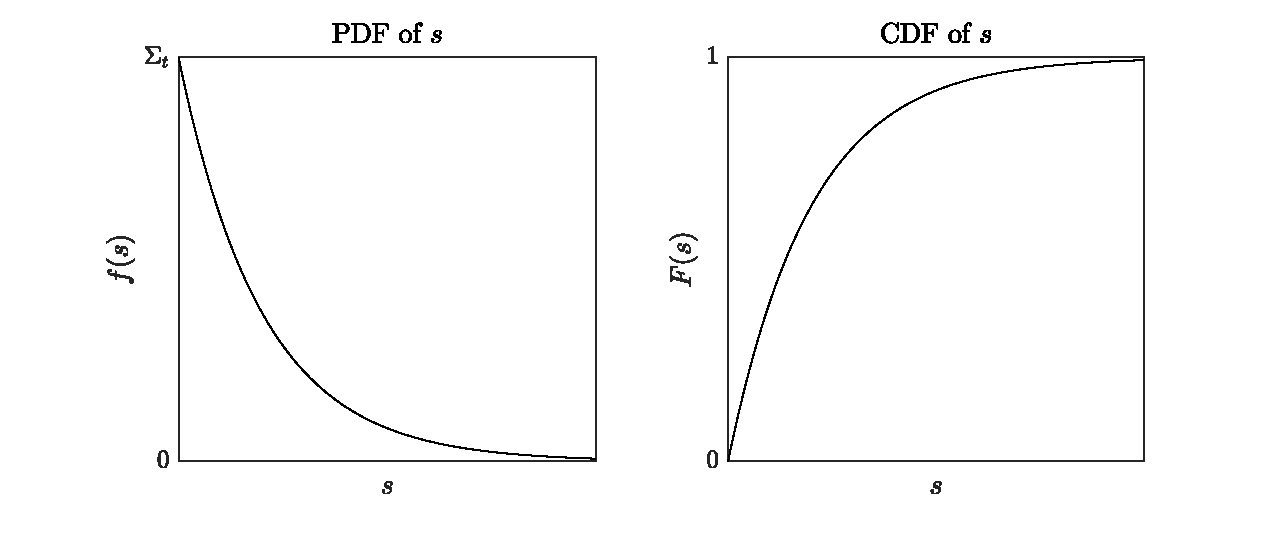
\includegraphics[scale=0.75]{images/cdf_pdf}
  \caption{Plots of the \acrshort{cdf} and \acrshort{pdf} for collision probability per distance travelled $s$.}
  \label{fig:cdf_pdf}
\end{figure}

As the \gls{cdf} ranges from zero to unity, we can sample its value by
a uniformly distributed random variable $\xi \in [0,1)$. The distance
traveled, $s$, referred to as the path length, can then be expressed as
a function of this sampled random variable:
\begin{align*}
  F(s) = 1 - e^{-s\Sigma_t} &= \xi \:,\\
  \ln(e^{-s \Sigma_t}) &= \ln(1-\xi)\:, \\
  -\Sigma_t s &= \ln(\xi) \:,\\
  s(\xi) &= \frac{1}{\Sigma_t}\ln(\xi)\:.
\end{align*}

After sampling the path length of the neutron, its position is
updated based on its original position and direction. We assumed that
the cross-section $\Sigma_t$ was constant in a material region, so the
sampled path length is only valid as long as the neutron remains in
that region.  If the neutron reaches the boundary between two material
regions, a new path length must be sampled using the cross-section of
the region it is entering. Each time a path length is sampled, the
distance to the nearest boundary in the direction of motion is
determined, and the neutron is moved to the boundary and path length
is resampled if appropriate. This can become computationally expensive
in complicated geometries and when the probability of crossing
boundaries with each sample path length is high.

\section{Woodcock Delta-tracking}
\label{sec:delta-tracking}

As discussed in Section~\ref{sec:ray_tracing}, the value of $\Sigma_t$
at a given position depends on the material at that point. Therefore,
$\Sigma_t(\vec{r})$ is a piece-wise discontinuous function that varies
arbitrarily with position and the geometry of the
problem~\cite{leppanen2013}. Using the ray tracing method, neutrons
must stop at boundaries to sample a new path length in a new material
region. To avoid the computational inefficiency that arises in
geometrically-complicated regions, a rejection sampling technique
known as Woodcock delta-tracking was developed~\cite{woodcock1965}.

Woodcock delta-tracking introduces the concept of the majorant
cross-section, chosen to be the maximum of all material total
cross-sections in the region of interest:
\begin{equation}
  \label{eq:majorant}
  \Sigma_\mathrm{maj} \equiv \max_{\mathbf{r} \in \mathbb{V}}\{\Sigma_t(\mathbf{r})\}\:,
\end{equation}
where $\mathbb{V}$ is the volume of interest. The majorant concept is shown in a
one-dimensional region in Fig.~\ref{fig:sigma_maj}.
\begin{figure}[hbt]
  \centering
  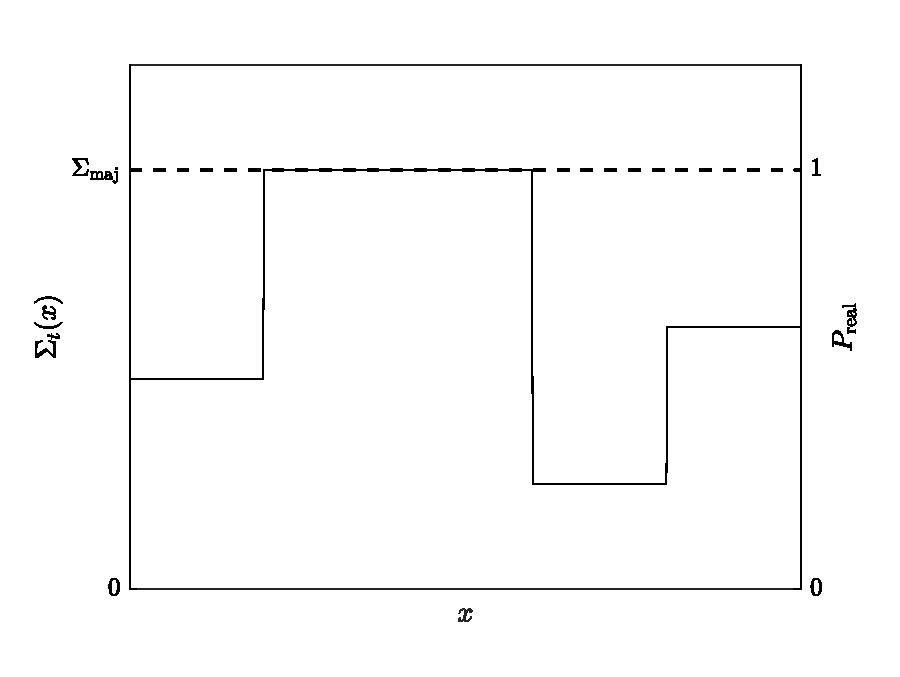
\includegraphics[scale=0.75]{images/sigma_maj}
  \caption{Total cross-section as a function of position in one
    dimension. The majorant cross-section is the largest value in the
    region of interest and determines the probability of a real collision.}
  \label{fig:sigma_maj}
\end{figure}
% should y axis be \Sigma_{t} for clarity? Updated -jsr

The majorant
cross-section can also be represented as the summation of the total
cross-section and a delta cross-section:
\begin{equation}
  \label{eq:majorant2}
  \Sigma_\mathrm{maj} = \Sigma_\delta(\mathbf{r}) +
  \Sigma_t(\mathbf{r}), \quad\forall \vec{r} \in \mathbb{V}\:.
\end{equation}
Following from the definition of $\Sigma_\mathrm{maj}$ in
Eq.~\eqref{eq:majorant}, the function $\Sigma_\delta(\mathbf{r})$ is
chosen such that $\Sigma_\mathrm{maj}$ is constant for the entire
region of interest. At the position \textbf{r} where the maximum value
of $\Sigma_t(\mathbf{r})$ occurs, the delta cross-section is zero.

The majorant cross-section is constant throughout the entire region of
interest, so we can treat it as a single material. Following the same derivation in
Section~\ref{sec:ray_tracing}, the \gls{pdf} of the first collision occurring after
$s$ in the region of interest using the majorant cross-section is given by:
\begin{align}
 f_{\mathrm{maj}}(s) &= \Sigma_{\mathrm{maj}}e^{-\Sigma_{\mathrm{maj}}s}\\
& = (\Sigma_{\delta}(\mathbf{r}) + \Sigma_{t}(\mathbf{r}))e^{-\Sigma_{\mathrm{maj}}s}\:.
  \label{eq:majorantpdf}
\end{align}

In most of the region of interest, the majorant cross-section is not
the real cross-section. To accurately preserve physics, we must use a technique called rejection
sampling to simulate sampling the real $\Sigma_t(\vec{r})$ while
actually sampling using $\Sigma_\mathrm{maj}$. 

\subsubsection{Rejection Sampling}
\label{sec:rejection_sampling}
As described by Lux and
Koblinger~\cite{lux1991}, rejection sampling requires a \gls{pdf} of
interest, $f(x)$, and a second \gls{pdf} $g(x)$ for which:
\begin{equation}
  \label{eq:Mleq}
  f(x) \leq M\cdot g(x), \quad \forall x\:,
\end{equation} where $M \in \mathbb{R}$ is a constant.
Sampling from $M\cdot g(x)$ and accepting these samples with probability:
\begin{equation}
  \label{eq:preal}
  P = \frac{f(x)}{M\cdot g(x)}
\end{equation}
replicates sampling directly from $f(x)$. 

For example, consider a
\gls{pdf} of interest $f(x) = x^2$ on the interval $x \in (0,1]$ as shown
in Fig.~\ref{fig:circle_square}.
\begin{figure}[hbt]
  \centering
  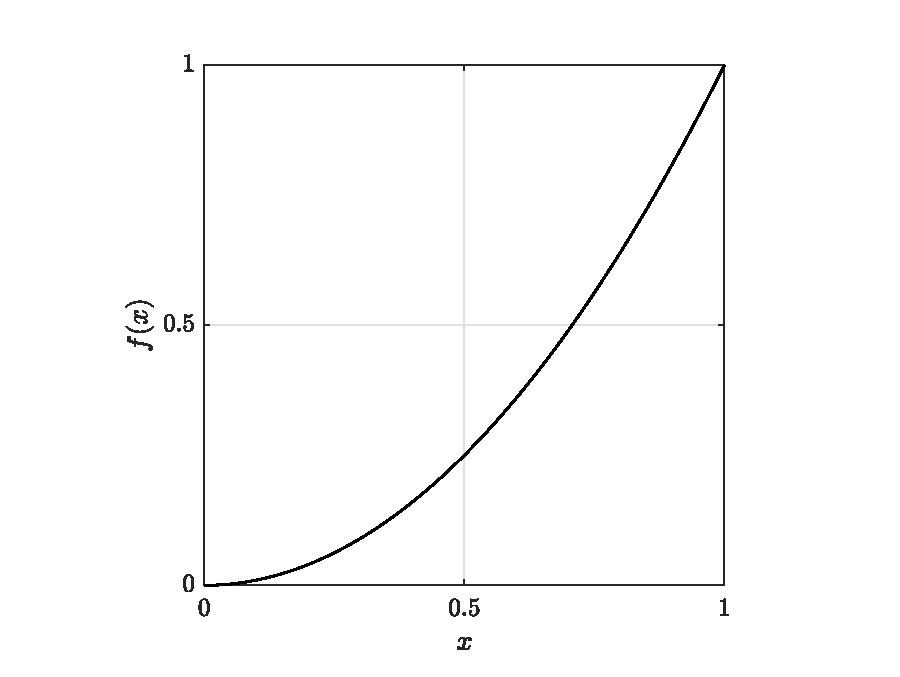
\includegraphics[scale=0.75]{images/circle}
  \caption{Example \acrshort{pdf} function $f(x) = x^2$.}
  \label{fig:circle_square}
\end{figure}
As described in the previous section, we could sample $f(x)$ using the
$F(x)$ found by integrating and then inverting. Instead, we can sample from a
different \gls{pdf} that is always majorant of $f(x)$, as defined in
Eq.~\eqref{eq:Mleq}. We can choose $g(x) = M = 1$, as $f(x) \leq 1$ on
the interval of interest. The \gls{cdf} of $g(x)$ is easy to
determine, because it is a constant value, and is just $G(x) =
x$. Therefore, we can sample $g(x)$ by simply sampling a random value $\xi
\in (0,1]$ and taking this as the value of $x$. To replicate sampling
from $f(x)$, we then sample another random value $\xi_2 \in (0,1]$ and
accept our value of $x$ using the probability defined in Eq.~\eqref{eq:preal}:
\begin{equation*}
  \xi_2 \leq \frac{f(x)}{M \cdot g(x)} = x^2\:.
\end{equation*}
% may what to mention that M=1 in this case?
\begin{minipage}{1.0\linewidth}
The following Matlab script replicates this procedure and generates
the histogram shown in Fig.~\ref{fig:pdf_histogram}.
\begin{lstlisting}
a = [];                     % Accepted samples
for i = 1:1000
    x = rand;               % Sample g(x)
    y = rand;               % Gen random number xi2
    if y <= x.^2            % If xi2 <= f(x)/g(x)
        a(end+1) = x;       % Accept sample
    end
end
\end{lstlisting}
\end{minipage}
As expected, the procedure has reproduced the desired \gls{pdf} of
$f(x) = x^2$. Although this requires sampling two random variables, it
can be advantageous if $F(x)$ is difficult or impossible to invert.
\begin{figure}[hbtp]
  \centering
  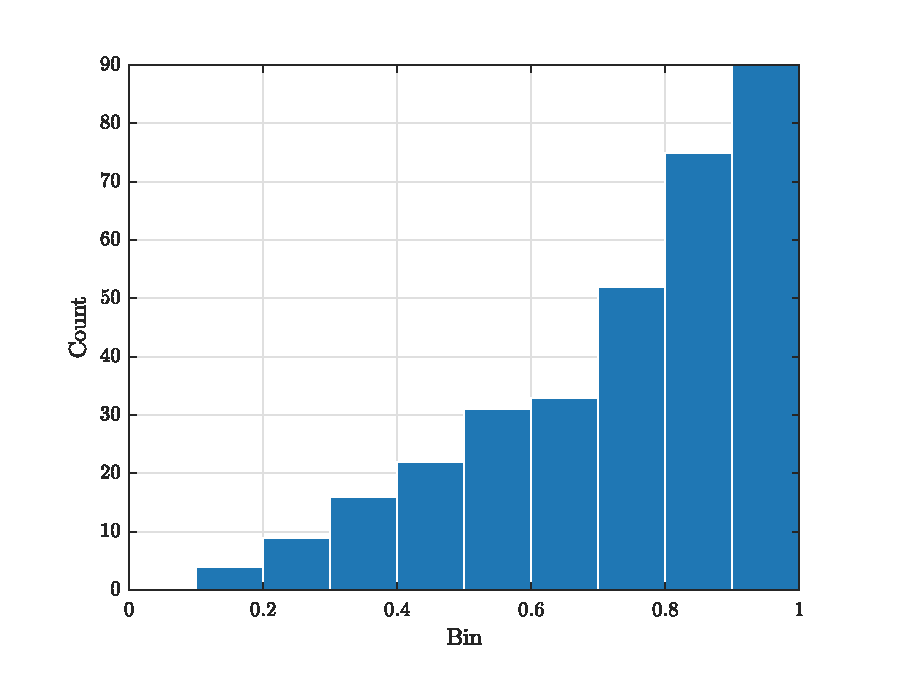
\includegraphics[scale=0.75]{images/pdf_histogram}
  \caption{Histogram of results from sampling and applying the
    rejection sampling algorithm.}
  \label{fig:pdf_histogram}
\end{figure}
\subsubsection{Application to Delta-tracking}
\label{sec:application_to_delta-tracking}

As we saw in Fig.~\ref{fig:sigma_maj}, the total cross-section
$\Sigma_t$ is a piecewise discontinuous function that depends on the
geometry of our problem. Therefore, each region has a different
\gls{cdf} for sampling path length, and described in
Section~\ref{sec:ray_tracing}. Using rejection sampling, we can sample
the real collision \gls{pdf}, using a different, simpler \gls{pdf}.
In Woodcock delta tracking, the second \gls{pdf}, $g(x)$, is chosen to
be the majorant \gls{pdf}, Eq.~\eqref{eq:majorantpdf}. This is
beneficial because the majorant cross-section is constant over the
entire region.

These functions are both maximized at $x=0$, where the inequality of
Eq.~\eqref{eq:Mleq} is satisfied by setting $M=1$:
\begin{equation}
  \label{eq:cseq}
  \Sigma_t(\mathbf{r}) \leq \Sigma_\mathrm{maj}(\mathbf{r}), \forall
  \mathbf{r} \in \mathbb{V} \:.
\end{equation}
We sample path length using the constant majorant
cross-section:
\begin{equation}
  \label{eq:majorantsample}
  s_\mathrm{maj}(\xi) = -\frac{1}{\Sigma_\mathrm{maj}}\ln(\xi)\:,
\end{equation}
which samples the \gls{pdf} defined in Eq.\eqref{eq:majorantpdf}.
% don't need to repeat equation; I think you mean this eqref?
% Can you clarify this comment? -jsr
We can see that this \gls{pdf} is the sum of two different ones: one
representing actual collisions based on the real total cross-section
$\Sigma_t$ and one representing the non-physical collisions based on
$\Sigma_\delta$. We call these non-physical collisions ``virtual''
collisions, and these should be eliminated by our rejection
sampling. To apply rejection sampling, we therefore pick the \gls{pdf}
we want to sample, $f(x)$, and the \gls{pdf} we will actually sample,
$g(x)$, as such:
\begin{align*}
  f(x) &= \Sigma_t(\vec{r})e^{-\Sigma_\mathrm{maj}s} \:,\\
  g(x) &= \Sigma_\mathrm{maj}e^{-\Sigma_\mathrm{maj}s}\:.
\end{align*}
The equation $g(x)$ is always majorant to $f(x)$, by the definition of
$\Sigma_{\mathrm{maj}}$, so we set $M=1$. We will therefore accept samples with the
probability given in Eq.~\eqref{eq:preal}:
\begin{align}
  \label{eq:prealfinal}
  P_{\mathrm{real}}(\vec{r}) &= \frac{f(x)}{M \cdot g(x)} =
      \frac{\Sigma_t(\mathbf{r})e^{-\Sigma_\mathrm{maj}s}}{\Sigma_\mathrm{maj}e^{-\Sigma_\mathrm{maj}s}}
  = \frac{\Sigma_t(\mathbf{r})}{\Sigma_\mathrm{maj}}\:.
\end{align}
% what's M?
We will refer to this as the probability of a ``real'' collision,
$P_\mathrm{real}$, to differentiate these physical collisions from the
non-physical virtual collisions. It is important to note that the
probability is independent of path length $s$, but is dependent on
position $\vec{r}$. At each collision, the material region at the
neutron position must be determined, but we do not need to explicitly
track boundaries nor calculate their distance each time a path length
is sampled. The algorithm for delta-tracking is shown in
Fig.~\ref{fig:dt}.

\begin{figure}[p]
  \centering
  \begin{algorithm}[H]
\caption{Delta-tracking}\label{alg:dt}
\begin{algorithmic}[1]
  \State \textbf{Sample} path length

  \State \textbf{Look up} location to get $\Sigma_t(\vec{r})$
  \State $P_\mathrm{real} \gets
  \frac{\Sigma_t(\vec{r})}{\Sigma_\mathrm{maj}}$
  \State \textbf{Sample} random number $\xi \in [0,1)$
  \If{$\xi < P_\mathrm{real}$} \Comment{Collision is real}
  \State \textbf{Execute} real collision
    \Else \Comment{Collision is virtual}
    \State \textbf{Execute} virtual collision
  \EndIf
\end{algorithmic}
\end{algorithm}
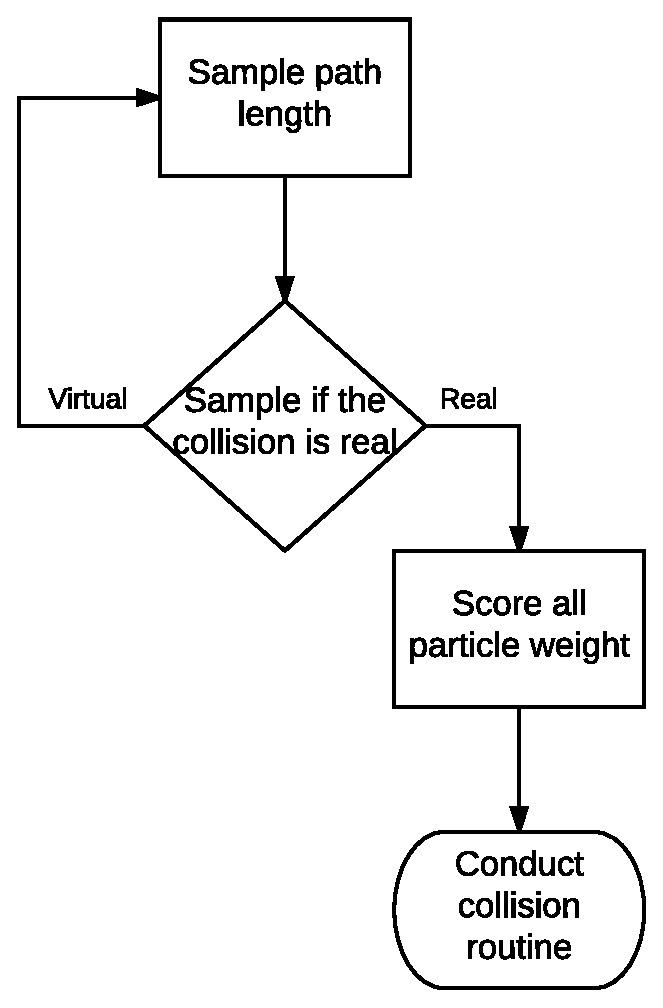
\includegraphics[scale=0.5]{images/dt}
  \caption{Delta-tracking algorithm and flow chart.}
  \label{fig:dt}
\end{figure}

Now, the path length can be sampled across multiple material regions
of varying $\Sigma_t$ without explicitly stopping the neutron at a
given boundary. This allows us to avoid determining the distance to
the nearest boundary after each path length sampling. Delta-tracking
is also much more efficient in regions where the geometry is complex
or material region thicknesses are on the same order as the path
length.% I'd add a sentence about why this is important--make us see that this is a thing it is
% a good idea to choose sometimes; the imbalance in talking about the negative
% properties leaves me wondering why anyone would choose it.
This method can become computationally inefficient in
regions where the total cross-section is much less than the majorant
cross-section, leading to oversampling of virtual collisions. This is
seen in geometries that include localized absorbers, such as control
rods.

% Another downside is that the \gls{tle} for
% flux cannot be used. 
% % Apparently this isn't true. I didn't get the details, but this came up for Kelly at M&C
% % Check with her to see if she found the reference about it. 
% The \gls{tle} requires calculating the track-lengths
% within a particular material cell, and therefore does not work when
% the neutron path length can cross one or more material
% boundaries. The \gls{cfe} can be used in its
% place, but often results in inferior statistics as not every track
% length sampled ends in a collision~\cite{leppanen2013}.
% % May want to elaborate on all of this, but it'll likely change
% given previous comment. 
%
% I commented it out, I'll email Jaakko about his paper, which I use
% as a reference for it. - JSR

\section{The Serpent 2 Monte Carlo Code}
\label{sec:serpent2}

The Serpent Monte Carlo code was developed at \gls{vtt} as a PhD
thesis project~\cite{leppanen2007}. A second iteration of the code,
Serpent 2, is currently under development. Both versions of Serpent use a combination of surface tracking, Woodcock
delta-tracking, and rejection sampling for non-uniform density
distributions. Serpent 2 selects between surface tracking and
delta-tracking by examining the ratio of total cross-section to
majorant cross-section~\cite{leppanen2010}. In regions where many
virtual collisions would occur, the code preferentially switches to
ray tracing. This is to avoid the computational inefficiency of
processing virtual collisions that provide no statistics. This
selection is determined by a constant $c$ and the inequality in
Eq.~\eqref{eq:s2deltasurface}.
\begin{equation}
  \label{eq:s2deltasurface}
  \frac{\Sigma_t(\vec{r})}{\Sigma_\mathrm{maj}} > 1 - c
\end{equation}

If this inequality is true, delta-tracking is used, otherwise
ray-tracing (referred to as surface-tracking in Serpent 2) is used. By
default, the value of $c$ is 0.9, as this was determined to produce
the best improvement in run time~\cite{leppanen2010}. We note that
this inequality is identical to the value of $P_\mathrm{real}$. Prior to
sampling path length, the code tests this ratio for the current
neutron position and determines if surface tracking or delta-tracking
should be used. If delta-tracking is used, the code then determines if
the collision is virtual or real. The value of $c$ can be set in the
input file using \verb|set dt|.
% \begin{figure}[hbtp]\centering
%   \begin{tikzpicture}[scale=1.5]
%     \draw[thick] (0,0) -- (10.0,0);
%     \foreach \x in {0,1,...,10}
%     {
%       \draw (\x, 0.1) -- (\x, -0.1);
%       \pgfmathsetmacro\result{\x * 0.1}
%       \node [below] at (\x, -0.2) {\small $\pgfmathprintnumber{\result}$};
%     }
%     \node [left] at (0,0) {$P_{\mathrm{real}}$};
%     \draw[ thick, <->] (0,0.2) -- (1,0.2);
%     \draw[ thick, <->] (1,0.2) -- (10,0.2);
%     \node [above] at (0.5, 0.2) {Ray Tracing};
%     \node [above] at (5.5, 0.2) {Delta-tracking};
%   \end{tikzpicture}
%   \caption{Ray-tracing and delta-tracking threshold values in
%     standard Serpent 2.}
%   \label{fig:ray_wdt_normal}
% \end{figure}
% Not sure that this is really illustrating anything.

% \subsubsection{Nonuniform Density Distributions}
% \label{sec:nonuniform}

% Rejection sampling can also be used when the total cross-section is
% not constant within a material region. As discussed by
% Lepp\"{a}nen~\cite{leppanen2013}, Serpent 2 conducts a rejection
% sampling routine similar to Woodcock delta-tracking in these
% regions. Instead of sampling from a majorant cross-section across
% multiple materials, a maximum cross-section for the single material
% region is used. Unlike delta-tracking, this requires stopping the
% neutron at boundaries and resampling path lengths. This algorithm is
% not modified by the implementation of \gls{wdt} and none of the input
% files used to assess \gls{wdt} use this feature.
% Wait, maybe I missed something, but I don't know what's going on this section / paragraph.
%
% This is extraneous and outside the scope of this. Not even sure why
% I put it in here. -JSR

%%% Local Variables:
%%% mode: latex
%%% TeX-master: "../masters_report"
%%% End:

\chapter{Method}
\label{chap:method}

The Serpent 2 Monte Carlo code uses a combination of  ray tracing and
delta-tracking to simulate the propagation of particles. The \gls{wdt}
method modifies delta-tracking for an absorbing medium, replacing virtual
collisions with a weight reduction. In this chapter, we will discuss
the \gls{wdt} routine for absorption events, and extend the method to
include scattering. We will then define the \gls{wdt} threshold, a key
parameter for its implementation in Serpent 2.

\section{\Acrlong{wdt}}
\label{sec:wdt}

Morgan and Kotlyar~\cite{morgan2015} introduced a method to improve the
inefficiencies of Woodcock delta-tracking in the presence of large
absorbers. The method, \gls{wdt}, replaces the
rejection sampling algorithm of delta-tracking with a weight reduction
algorithm. This process is similar to survival biasing, or implicit capture.

\subsection{Implicit Statistical Events}
\label{sec:implicit}

We consider a process that can result in multiple outcomes, each with
their own probability. One approach is to sample a random variable and
determine which outcome actually occurred. If the event occurs many
times, we can instead replace the
statistical process by using the expected value of the random process
\cite{lux1991}. The expected value of a random variable $x$ that can
take values ${x_1 \ldots x_n}$ with  probabilities ${p_1 \ldots p_n}$, respectively,
is given by:
\begin{equation}
  \label{eq:expval}
  E[x] = x_1p_1 + x_2p_2 \ldots + x_{n}p_n
\end{equation}
For example, imagine we have a bag with four coins, three worth \$0.25 and
one worth \$0.10. The values and their probabilities are:
\begin{align*}
  x_1 = 0.25, \quad p_1 = \frac{3}{4} = 0.75 \\
  x_2 = 0.10, \quad p_2 = \frac{1}{4} = 0.25
\end{align*}
For a given draw, we could sample a random value and use the
probabilities $p_1$ and $p_2$ to determine the coin drawn. Or, we can
describe the expected value of the drawn coin:
\begin{align*}
  E[x] &= x_1p_1 + x_2p_2 \\
  &= (0.25 \times 0.75) + (0.10 \times 0.25) \\
  &= 0.2125
\end{align*}
\begin{minipage}{1.0\linewidth}
  This value represents the average value of a coin drawn, if we
  perform many draws. The following Matlab code replicates this
  procedure:
\begin{lstlisting}
v = 0;
n = 1000;
for i = 1:n
    xi = rand;  
    v = v + (xi < 0.25)*0.1 + (xi >= 0.25)*0.25;
end
\end{lstlisting}
\end{minipage}

Although the exact values will vary due to the small sample size, \verb|v/n|
$\approx 0.2125$, as we expected.

This framework is often applied to neutron propagation in a process
called ``survival biasing.'' At each collision location, the type of
interaction is sampled and the appropriate action taken. In the case
of an capture event the neutron is ``killed,'' removed from the
simulation. While this accurately reflects the physical reality, it
does not produce good statistics. Assuming we are using a collision
estimator, the neutron's contribution to our simulation is the history
of collisions. Each of these provide a score to that particular
collision, contributing to the overall simulation
statistics. Capture events that kill neutrons, therefore, are
removing the very particles we need to generate better statistics,
resulting in the need for many more particles. Mitigating this issue
is the goal of survival biasing.

Survival biasing avoids killing neutrons by replacing capture
events with an expected outcome. As described above, we do not need to
track the outcome of every single event, but can rely on the expected
value. This will give us, on average, the outcome of our many
events. To eliminate our explicit consideration of capture events,
we therefore have two possible event types: capture events, and
scattering events. The probabilities $p$ will be given by the
ratios of the cross-sections:
\begin{align*}
  p_{\mathrm{capture}} = \frac{\Sigma_{c}}{\Sigma_t} \\
  p_{\mathrm{scattering}} = \frac{\Sigma_{s}}{\Sigma_t}
\end{align*}
Where $\Sigma_{c}$ and $\Sigma_{s}$ are the macroscopic cross-sections
for capture and scattering, respectively.

In the coin example, each had a different monetary value, giving us an
expected value when we drew many times. We must introduce something
similar for neutrons. It is convention to call this intrinsic value
``weight'' and represents the importance of the neutron. All neutrons
are born with the same weight, usually unity, and are killed when they
have zero weight. By that convention a capture event that kills a
neutron immediately forces the final weight of the neutron to zero,
$w_{f,\mathrm{capture}} = 0$. We can then calculate the expected
value of the interaction of a neutron with initial weight $w_i$:
\begin{align*}
  E[w_f] &= w_{f,\mathrm{scattering}}p_\mathrm{scattering} +
           w_{f,\mathrm{capture}}p_\mathrm{capture} \\
  &= w_{f,\mathrm{scattering}}p_\mathrm{scattering}
\end{align*}
A scattering event merely changes the location of the neutron in
energy and angle phase space, leaving its importance
unchanged. Therefore, $w_{f,\mathrm{scattering}} = w_i$:
\begin{align*}
  E[w_f] = w_ip_\mathrm{scattering} 
\end{align*}
Now every collision is considered to be a non-capture event. The
neutron continues with a lower weight, proportional to the probability
that the event was scattering. The weight lost in the collision is
scored as capture:
\begin{align*}
  S_\mathrm{capture} &= E[w_i - w_f] \\
  &= E[w_i] - E[w_f] \\
&= w_i - w_ip_\mathrm{scattering} \\
&= w_i(1-p_\mathrm{scattering})
\end{align*}
A similar method will be used by weighted delta-tracking.

\subsection{Russian Rouletting}
\label{sec:rouletting}

When the survival biasing routine described in Sec.~\ref{sec:implicit}
is used, the loss of neutrons is entirely reliant on leakage from the
problem or fission events. Neutrons will continue to undergo
collisions and subsequent weight reduction until they have a very low
weight. These particles will only contribute small amounts to our
statistics, so tracking them is computationally inefficient.  To
mitigate this, a lower cutoff for the weight is introduced. Once
neutrons are below this weight, they have a chance of being killed by
a Russian Rouletting routine. The general algorithm is shown in
Algorithm~\ref{alg:roulette}.
\begin{algorithm}
\caption{Rouletting Routine}\label{alg:roulette}
\begin{algorithmic}[1]
\If{weight $<$ weight threshold}
   \State $\xi \gets $ random number $\in [0,1)$
   \If{$\xi < $ roulette probability}
     \State Kill particle
   \Else
     \State $w_f \gets w_i$/(roulette probability) \label{inc}
   \EndIf
\EndIf
\end{algorithmic}
\end{algorithm}
Following a collision, if the weight of the colliding particle is
below a defined weight threshold, a random number is sampled. If this
number is below a defined rouletting probability, the particle is
killed. If the particle survives rouletting, its weight is increased
proportional to the rouletting probability. By killing low weight
particles, or increasing their weight, the inefficiency of tracking
low-weight particles can be reduced.

\subsection{\Acrlong{wdt}}
\label{sec:wdttheory}

Morgan and Kotlyar~\cite{morgan2015} introduced a method to improve
the inefficiencies of Woodcock delta-tracking in the presence of large
absorbers. The method, \gls{wdt}, replaces the rejection sampling of
delta-tracking with a weight reduction. This is similar to the process
of implicit capture discussed in Section~\ref{sec:implicit}.

The \gls{wdt} method samples the particle path length in the same fashion as
Woodcock delta-tracking. As described in Section~\ref{sec:delta-tracking},
after each path length sampled, the delta-tracking method accepts the
collision as real with the probability shown in
Eq.~\ref{eq:preal}. The \gls{wdt} method bypasses this rejection sampling by
accepting all collisions as real with a subsequent reduction in
weight. As discussed in Section~\ref{sec:implicit}, replacing a
statistical event requires calculation of the expectated value. In
this case, the two events are a real collision and a virtual
collision.
\begin{equation}
  \label{eq:wdtexpected}
  E[w_f] = w_{f,\mathrm{real}}P_{\mathrm{real}} + w_{f,\mathrm{virt}}P_{\mathrm{virt}}
\end{equation}
Morgan and Kotlyar examine a 1D test case with absorption. As an
absorption event removes the particle, the resulting final weight of a
real collision is zero. A virtual collision is rejected, and therefore
leaves the weight unchanged. Inserting the appropriate values into
Eq.~\eqref{eq:wdtexpected} gives the expected value of the final
weight for an absorption event.
\begin{align*}
  \label{eq:mkexpected}
  E[w_f] &= w_{f,\mathrm{real}}P_{\mathrm{real}} +
           w_{f,\mathrm{virt}}P_{\mathrm{virt}} \\
  &= 0 + w_iP_{\mathrm{virt}} \\
  &= w_i(1-P_\mathrm{real}) \\
  &= w_i\left(1-\frac{\Sigma_t}{\Sigma_\mathrm{maj}}\right)
\end{align*}
The particle that is left following the collsion continues propegating
as if it underwent a virtual collision. In this case, the absorption
is then scored using the expectation value of the score.
\begin{align*}
  S_\mathrm{absorption} &= E[w_i - w_f] \\
  &= E[w_i] - E[w_f] \\
  &= w_i\left(\frac{\Sigma_t}{\Sigma_\mathrm{maj}}\right)
\end{align*}
This is implemented by Kotlyar and Morgan in a 1D problem and the
results are verified with the analytical solution. The authors point
out that a rouletting routine should be implemented when this is used,
to prevent the tracking of low-weight neutrons.

\section{\Acrlong{wdt} with scattering}
\label{sec:wdt_scattering}


In a scattering event, the weight of the incident particle does not
change. Therefore, application of the expectation value as in
Section~\ref{sec:wdttheory} results in an expected value of the final
weight equal to the initial weight.
\begin{align*}
  E[w_f] &= w_{f,\mathrm{real}}P_{\mathrm{real}} +
           w_{f,\mathrm{virt}}P_{\mathrm{virt}} \\
  &= w_iP_\mathrm{real} + w_iP_{\mathrm{virt}} \\
  &= w_i(P_\mathrm{real} + 1 -P_\mathrm{real}) \\
  &= w_i
\end{align*}

This doesn't model what we expect. We can view \gls{wdt} as splitting
the weighted neutron into two particles. One carries the real portion
of the weight and experiences the collision. The other carries the
virtual portion of the weight and continues propagating as if no
collision occurred. This works fine for absorption, where the portion
that experiences the collision does not propagate, it is immediately
killed and scored. But, when the neutron is split into a scattering
portion and a virtual portion, no weight is lost because neither of
those events change the weight.

Therefore, extension of this methodology to scattering requires duplication of
the particle at the point of collsion. The virtual portion of the
weight is carried away by a particle that propagates as if no
collision has occured, and the real portion is carried away by a
particle that undergoes scattering. In problems with scattering, this
results in a rapid multiplication of neutrons. When implemented into
Serpent 2, this multiplication very quickly filled any available
neutron buffer in simulations of a \gls{bwr}, ending
the simulation. Another method for handling scattering events must be
developed.

\subsection{Scattering Rejection Sampling}
\label{sec:scattering}

As described in the last section, the \gls{wdt} method may result in
an intractable simulation when applied to scattering. To maintain
proper statistics, scattering must take into account the possibility
of a virtual collision while using delta-tracking. To achieve this
goal, the delta-tracking rejection sampling that had been supplanted
by \gls{wdt} was moved into the scattering subroutine. Therefore, the
new routine uses both rejection-sampling and implicit events to
account for the possibility of real and virtual collisions. The
algorithm is shown in Alg.~\ref{alg:scattalg} and a flow chart of the
routine is shown in Fig.~\ref{fig:wdt}

\begin{figure}[p]
\begin{algorithm}[H]
\caption{\Acrlong{wdt} with scattering}\label{alg:scattalg}
\begin{algorithmic}[1]
  \State \textbf{Sample} path length
  \State \textbf{Sample} collision type
  \If{collision type == (capture or fission)}
    \State \textbf{Score} capture or fission $\gets
    w_iP_\mathrm{real}$
    \State \textbf{Score} collision  $\gets w_iP_\mathrm{real}$
    \State $w_f \gets w_i(1-P_\mathrm{real})$
    \State \textbf{Execute} virtual collision
  \Else
    \State \textbf{Sample} random number $\xi \in [0,1)$
    \If{$\xi < P_\mathrm{real}$} \Comment{Collision is real}
    \State \textbf{Score} scattering $\gets w_i$
    \State \textbf{Score} collision $\gets w_i$
      \State \textbf{Execute} scattering collision
    \Else \Comment{Collision is virtual}
    \State \textbf{Execute} virtual collision
    \EndIf
  \EndIf
\end{algorithmic}
\end{algorithm}
  \centering
  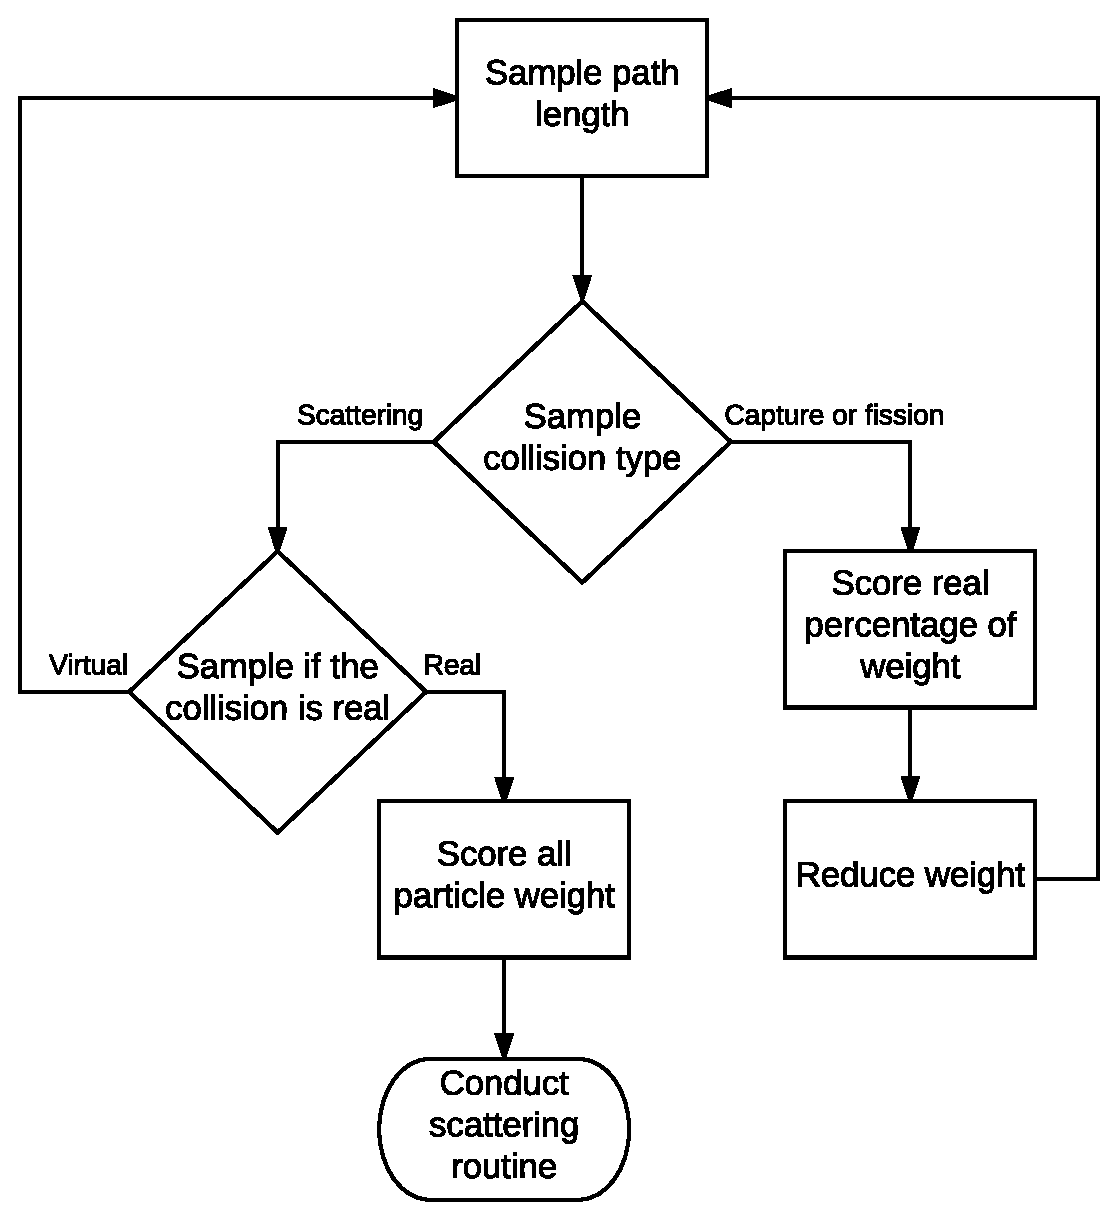
\includegraphics[scale=0.5]{images/wdt}
  \caption{\Acrlong{wdt} with scattering rejection sampling.\label{fig:wdt}}
\end{figure}
Note that there are two separate scoring events in each collision
subroutine: scoring of the actual collision type for calculating
specific reaction rates, and scoring of collision itself used by the
collision flux estimator. In addition, scoring the fission reaction
also encompasses generation of fission neutrons.

In the original delta-tracking routine, the rejection sampling takes
place prior to collision type sampling, and collision scoring can
occur between the two. This is the routine that Serpent 2 used, prior
to modification for the above scheme. By moving the rejection sampling
after the collision type sampling, the collision score is no longer
agnostic of the type of collision that will occur. Therefore, in the
implementation of this routine in Serpent 2, the collision scoring was
moved after the collision type sampling.

\section{Implementation in Serpent 2}
\label{sec:method_implementation}

The \gls{wdt} algorithm is implemented to work alongside the current
implementation of ray tracing and delta-tracking, as described in
Sec.~\ref{sec:serpent2}. \gls{wdt} is designed to improve the
effectiveness of delta-tracking when the change of a virtual collision
is high. We can hypothesize that the algorithm will benefit in the
regime where $P_{\mathrm{real}}$ is low. At high values of
$P_{\mathrm{real}}$, a majority of the weight of the incoming particle
is scored. This leaves the particle that undergoes a virtual collision
with a very low weight, relying on the rouletting routine to prevent
causing computational inefficiency. These two situations imply that
there is a region between low and high values of $P_\mathrm{real}$
where \gls{wdt} may provide benefit.

A new input parameter line \verb|set wdt| is used to indicate that
\gls{wdt} is to be used, and can also set the value of the \gls{wdt}
threshold $t_{\mathrm{wdt}}$. This is the ratio below which \gls{wdt} will be used. This
scheme is summarized in Fig.~\ref{fig:ray_wdt}.
\begin{figure}[hbtp]
  \centering
  \begin{align*}
    \mathrm{Mode} =
    \begin{cases}
      \mathrm{Ray tracing}, & P_\mathrm{real} < 1-c \\
      \mathrm{\gls{wdt}}, & 1-c \leq P_\mathrm{real} < t_{\mathrm{wdt}}
      \\
      \mathrm{Delta-tracking}, & P_\mathrm{real} \geq t_{\mathrm{wdt}}
    \end{cases}
  \end{align*}
  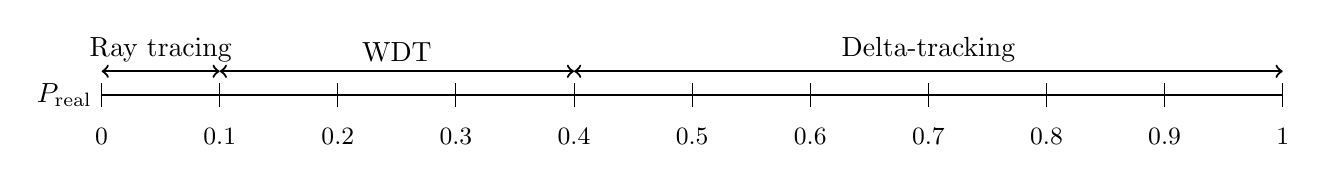
\begin{tikzpicture}[scale=1.5]
    \draw[thick] (0,0) -- (10.0,0);
    \foreach \x in {0,1,...,10}
    {
      \draw (\x, 0.1) -- (\x, -0.1);
      \pgfmathsetmacro\result{\x * 0.1}
      \node [below] at (\x, -0.2) {\small $\pgfmathprintnumber{\result}$};
    }
    \node [left] at (0,0) {$P_{\mathrm{real}}$};
    \draw[ thick, <->] (0,0.2) -- (1,0.2);
    \draw[ thick, <->] (1,0.2) -- (4,0.2);
    \draw[ thick, <->] (4,0.2) -- (10,0.2);
    \node [above] at (0.5, 0.2) {Ray tracing};
    \node [above] at (2.5, 0.2) {WDT};
    \node [above] at (7, 0.2) {Delta-tracking};
  \end{tikzpicture}
  \caption[Implemented selection scheme for ray-tracing, weighted and normal
    delta-tracking.]{Implemented selection scheme for ray-tracing, weighted and normal
    delta-tracking. Shown using the values of $(1-c)=0.1$ and $t_{\mathrm{wdt}}=0.4$.}
  \label{fig:ray_wdt}
\end{figure}



%%% Local Variables:
%%% mode: latex
%%% TeX-master: "../masters_report"
%%% End:

\chapter{Results}
\label{chap:results}
We expect that the \gls{wdt} method will improve the statistics of
Serpent 2 calculations. With normal delta-tracking, virtual collisions
provide no statistical benefit, and are therefore an inefficient use
of computational resources. Virtual collisions that results in
absorption events do contribute to statistics when using
\gls{wdt}. Therefore, we expect an improvement in the results of a
Serpent 2 simulation. In this section, we will describe how
performance in Serpent 2 is quantified, describe the three test cases,
and the results of those test cases.

\section{Performance metrics}
\label{sec:fom}

\subsection{Figure of Merit}
\label{sec:fom}

Monte Carlo codes such as Serpent 2 run many batches of a single
simulation, calculating the mean of values of interest $\hat{x}$
across the many runs. By the central limit theorem, we know that the
means across many simulations will form a normal distribution with
variance $\sigma^2(\hat{x})$. We are interested in reducing the
variance of the final value which will provide more confidence in the
simulation results. In general, running the simulation more times will
reduce this variance at the cost of requiring more computation
time. The variance is proportional to the number of cycles $n$:
\begin{equation}
\label{eq:variance}
  \sigma^2(\hat{x}) = \frac{C}{n}
\end{equation}
Therefore, when we seek to improve the quality of the
statistics, as with \gls{wdt}, we are seeking improved variance with
less cycles. To measure this, we must establish a \gls{fom}.
The standard \gls{fom} used by most simulations, described by Lewis
and Miller~\cite{lewis1993}, is shown in Eq.~\eqref{eq:fom}:
\begin{equation}
  \label{eq:fom}
  \mathrm{FOM} = \frac{1}{\sigma(\hat{x})^2T}
\end{equation}
where $T$ is the runtime of the simulation, $T = Cn$. The runtime is
proportional to the number of cycles $n$, plugging in
Eq.~\eqref{eq:variance}:
\begin{equation*}
  \mathrm{FOM} = \frac{1}{\sigma(\hat{x})^2T}} = \frac{C\cdot n}{n} = C
\end{equation*}


 A higher \gls{fom}
indicates higher accuracy per computation time, and therefore a more
efficient algorithm. Serpent 2 collects scores for each cycle (or
batch of cycles) and outputs the sample mean and standard
deviation\todo{Check if this is stdev or
  var}~\cite{VTT-R-00371-14}. This enables comparison of Serpent 2
running with and without \gls{wdt} to determine the efficiency of the
algorithm.

\subsection{Convergence}
\label{sec:convergence}

As described in the previous section, we expect the variance to
improve with further simulation. Fig.~\ref{fig:error_convergence}
shows the variance in the measurement of infinite flux,
$\phi_{\infty}$ as a function of Serpent 2 simulation cycles. As
shown, the variance decreases linearly as the simulation is run
further.
\begin{figure}[hbtp]
  \centering
  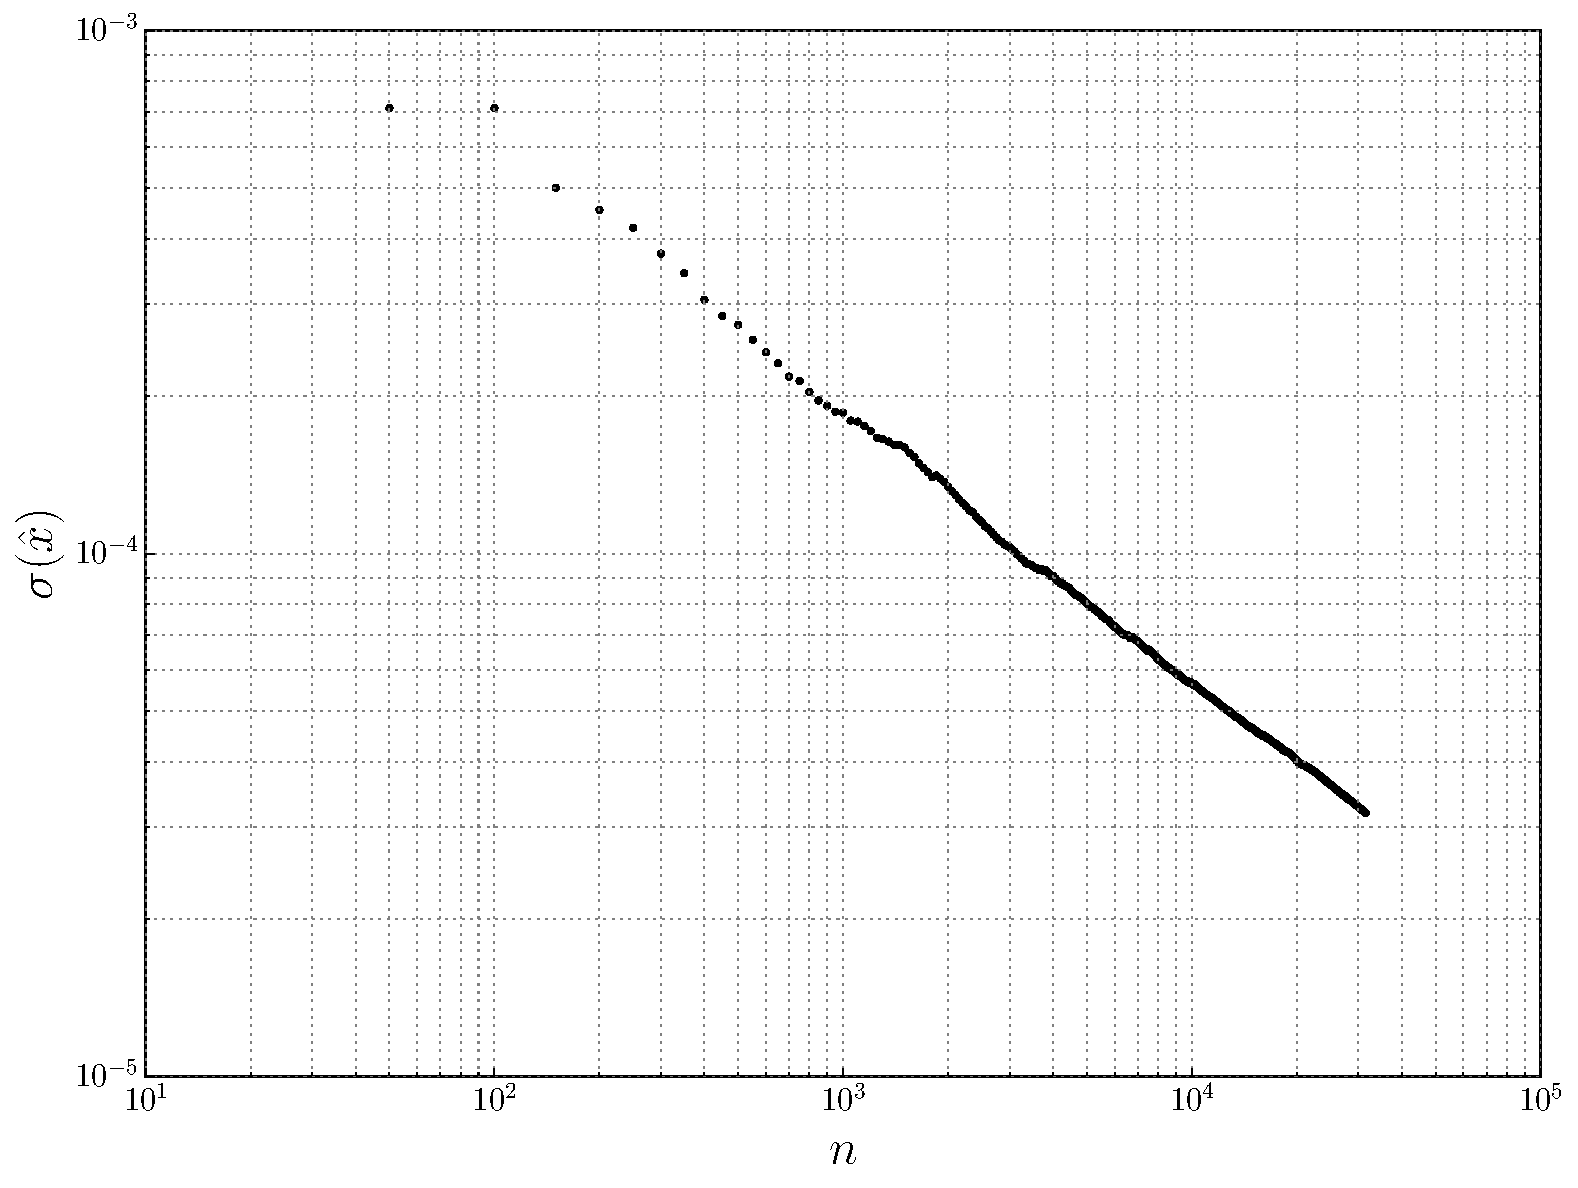
\includegraphics[scale=0.4]{images/error_convergence}
  \caption[Variance in $\phi_{\infty}$ for the fast-neutron group as a
    function of Serpent 2 cycle.]{Variance in $\phi_{\infty}$ for the fast-neutron group as a
    function of Serpent 2 cycle, with \gls{wdt} threshold of 0.2.}
  \label{fig:error_convergence}
\end{figure}

\begin{figure}[hbtp]
  \centering
  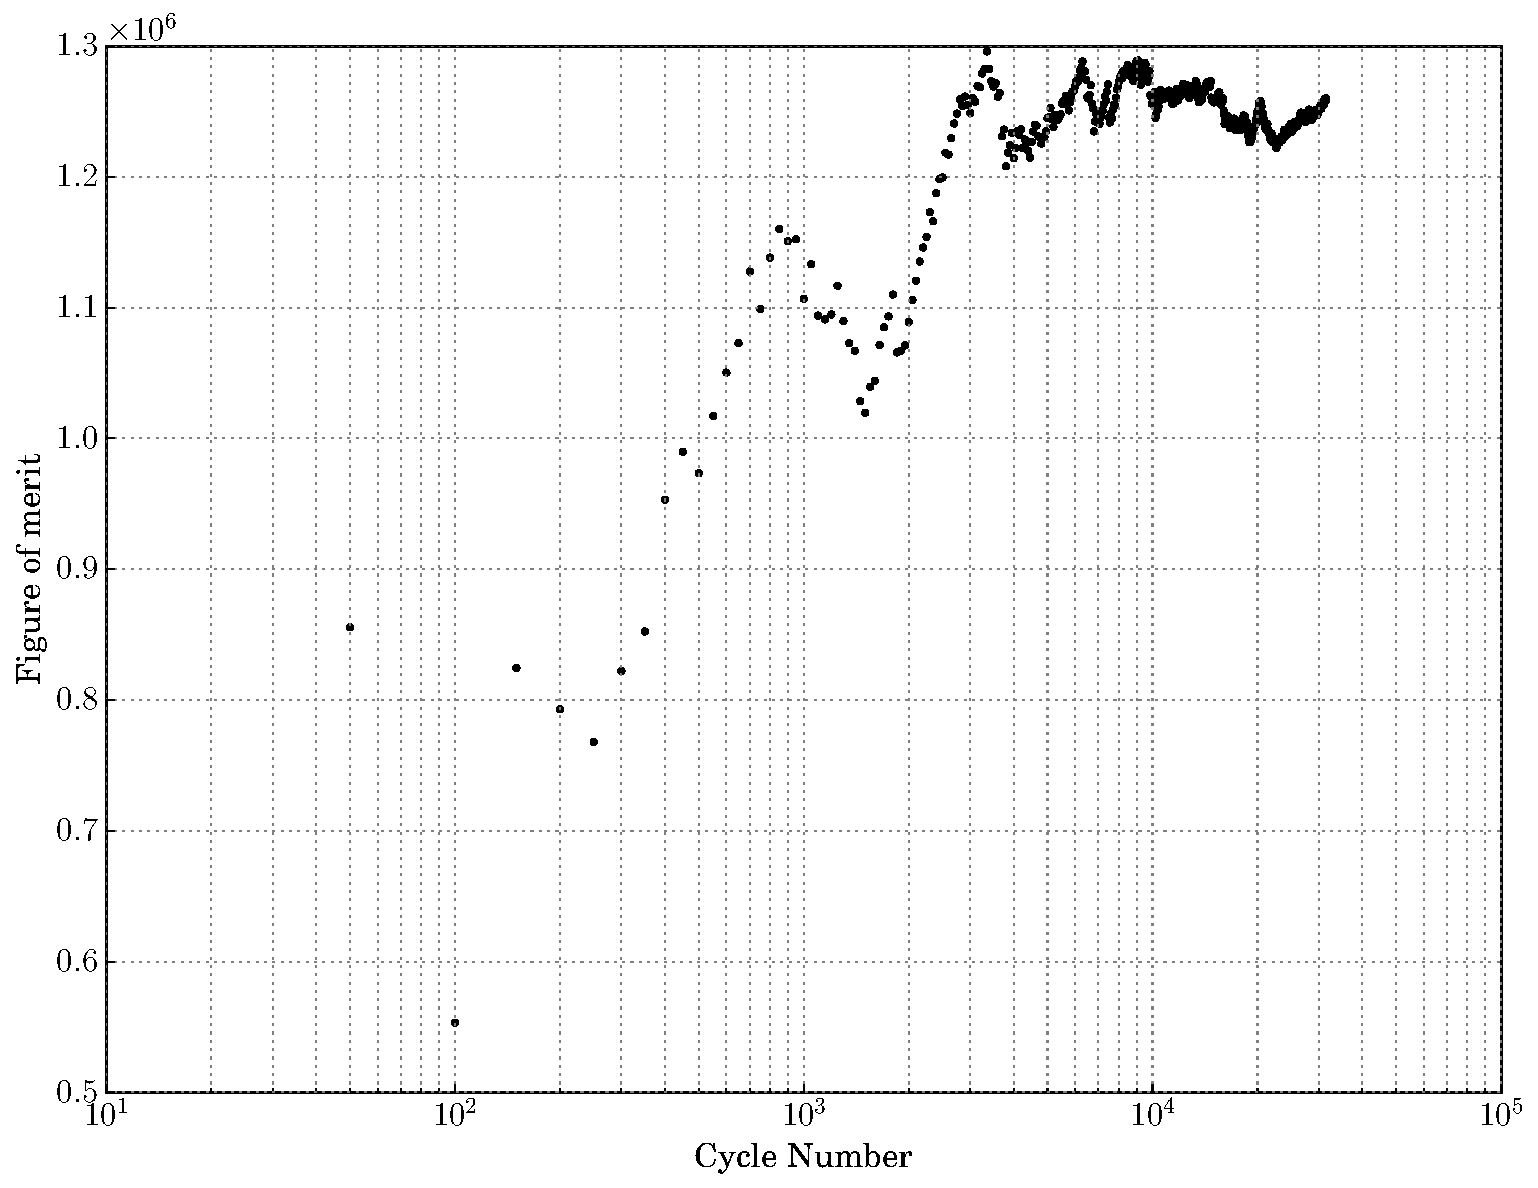
\includegraphics[scale=0.4]{images/fom_convergence_example}
  \caption[Figure of merit in $\phi_{\infty}$ for the fast-neutron group as a
    function of Serpent 2 cycle.]{Figure of merti in $\phi_{\infty}$ for the fast-neutron group as a
    function of Serpent 2 cycle, with \gls{wdt} threshold of 0.2.}
  \label{fig:fom_convergence}
\end{figure}

%% Convergence explanation

% Test Cases

%% PWR
%% Fast Pincell
%% Homog Element

%% -- Images

% Actual Results

%% Infinite flux

%% Cross-sections

%% Scattering matrices

%%% Local Variables:
%%% mode: latex
%%% TeX-master: "../masters_report"
%%% End:


\chapter{Conclusion}
\label{chap:conclusion}

% Overview of what was in the paper

\section{Summary of results}
\label{sec:results_summary}

For each test case, we examined three parameters: the infinite flux,
the total cross-section, and the scattering matrix for the zeroth
scattering moment. For the \gls{pwr} pin cell, we observed
improvements in the \gls{fom} for the thermal group in all three
parameters studied. A similar improvement was seen in the fast group
for the fast reactor pin cell. There is no indication of a clear trend
for the homogeneous fuel element.

Use of the \gls{wdt} method improved the \gls{fom} for the \gls{pwr}
and fast reactor pin cells in the groups that experience the most
absorption events. That is, the thermal group for the \gls{pwr} and
the fast group for the fast reactor. This is consistent with what we
expect from using the \gls{wdt} routine. With the original
delta-tracking routine, collisions that may result in absorption may
be discarded as virtual and therefore never scored. The \gls{wdt}
routine scores every collisions that results in absorption and reduces
the weight as necessary. This is a more efficient routine in energy
regions where absorption events are occurring at a high rate. The
additional scoring of absorption events improves the \gls{fom} for the
total cross-section; by not killing the neutrons at these events, the
\gls{fom} for flux is improved by survival biasing. 

In regions where a large amount of scattering occurs, the routine is
slightly less efficient. Instead of rejecting virtual collisions
outright, the rejection occurs after sampling the type of
collision. We observe the impact of this inefficiency in energy
regions where scattering dominates. The total cross-section and the
scattering matrices entries for the \gls{pwr} fast group both under
perform standard delta-tracking. The large amount of graphite in the
homogeneous fuel element makes it a highly scattering environment,
which may explain the under-performance in total cross-section of
\gls{wdt} in most cases.

We provide specific recommended values for the \gls{wdt} threshold in
the sections dedicated to the test cases. Overall, the method provides
some improvement in the \gls{fom} in circumstances where there is a
large amount of absorption, in line with what is expected of the method.

\section{Future Work}
\label{sec:future_work}

There is still a large amount of work to assess the usefulness and
performance of this method. Based on the results of this study, we
should assess test cases that have geometrically small regions of high
absorption, such as control rods. Also, test cases where
delta-tracking does not perform well, such as \gls{triso} particles,
should be analyzed. In addition to more test cases, adjusting the
upper boundary for ray tracing (see Fig.~\ref{fig:ray_wdt}) should be
analyzed. \Gls{wdt} may outperform ray tracing in some regions of very
low real collision probability. An expanded parametric study of
the \gls{wdt} threshold should be performed, to see if the general
trend observed here holds. This should include both a finer
examination of the \gls{wdt} threshold value, and examination of other
output parameters of interest.

\section{Conclusion}
\label{sec:conclusion}

In this manuscript, we have sought to determine the usefulness of the
\gls{wdt} method. We discussed the background of the Monte Carlo
simulation and how it is applied to neutral particle propagation. We
introduced Woodcock delta-tracking as a method to improve the
simulation in geometrically complex region. This algorithm was
modified by a recently introduced method, \acrlong{wdt}, which
replaced some virtual collisions with a weight reduction. We then
extended the method from considering only absorption events to include
scattering events. Finally, we examined three parameters of interest
from three test cases to assess the usefulness of \gls{wdt} and
determine a preferred threshold value for use of the algorithm. The
\gls{fom} improvements are in line with what was expected of the
\gls{wdt} method. The suggested future work should improve our
understanding of the impact of the method, and provide more robust
recommendations for future simulations.

%%% Local Variables:
%%% mode: latex
%%% TeX-master: "../masters_report"
%%% End:


\appendix


\chapter{Supplemental Data}
\label{chap:homog_data}

The homogenous fuel element simulations used eleven energy
groups. Printing all the data tables in the main body of the report
is therefore unsuitable. The full data is presented here and available
at the following link: \url{https://github.com/jsrehak/wdt_data/}

\begin{landscape}
  \section{Infinite flux}
\label{sec:homog_inf_flx_data}

\resizebox{1.2\textwidth}{!}{
\begin{tabular}{cccc}
  Group 1  & Group 2 & Group 3 & Group 4 \\
  \begin{tabular}{lrr}
\toprule
$t_{\mathrm{wdt}}$ & $\overline{\mathrm{FOM}}$ &    Ratio \\
\midrule
               0.1 &   2.019388$\times 10^{4}$ & 1.000000 \\
               0.2 &   2.087831$\times 10^{4}$ & 1.033893 \\
               0.3 &   2.205485$\times 10^{4}$ & 1.092155 \\
               0.4 &   2.190425$\times 10^{4}$ & 1.084697 \\
               0.5 &   2.123522$\times 10^{4}$ & 1.051567 \\
               0.6 &   2.074022$\times 10^{4}$ & 1.027055 \\
               0.7 &   2.038235$\times 10^{4}$ & 1.009333 \\
               0.8 &   2.059303$\times 10^{4}$ & 1.019766 \\
               0.9 &   2.055086$\times 10^{4}$ & 1.017678 \\
               1.0 &   2.179478$\times 10^{4}$ & 1.079276 \\
\bottomrule
\end{tabular}
 &
  \begin{tabular}{lrr}
\toprule
$t_{\mathrm{wdt}}$ & $\overline{\mathrm{FOM}}$ &    Ratio \\
\midrule
               0.1 &   1.774919$\times 10^{5}$ & 1.000000 \\
               0.2 &   1.765739$\times 10^{5}$ & 0.994828 \\
               0.3 &   1.740788$\times 10^{5}$ & 0.980770 \\
               0.4 &   1.843099$\times 10^{5}$ & 1.038413 \\
               0.5 &   1.775834$\times 10^{5}$ & 1.000516 \\
               0.6 &   1.775154$\times 10^{5}$ & 1.000132 \\
               0.7 &   1.726067$\times 10^{5}$ & 0.972476 \\
               0.8 &   1.751299$\times 10^{5}$ & 0.986692 \\
               0.9 &   1.691347$\times 10^{5}$ & 0.952915 \\
               1.0 &   1.879980$\times 10^{5}$ & 1.059192 \\
\bottomrule
\end{tabular}
 &
  \begin{tabular}{lrr}
\toprule
$t_{\mathrm{wdt}}$ & $\overline{\mathrm{FOM}}$ &    Ratio \\
\midrule
               0.1 &   2.114826$\times 10^{5}$ & 1.000000 \\
               0.2 &   2.081977$\times 10^{5}$ & 0.984467 \\
               0.3 &   1.999475$\times 10^{5}$ & 0.945456 \\
               0.4 &   2.165336$\times 10^{5}$ & 1.023883 \\
               0.5 &   2.118403$\times 10^{5}$ & 1.001691 \\
               0.6 &   2.075683$\times 10^{5}$ & 0.981491 \\
               0.7 &   1.978024$\times 10^{5}$ & 0.935313 \\
               0.8 &   2.050604$\times 10^{5}$ & 0.969632 \\
               0.9 &   2.021991$\times 10^{5}$ & 0.956102 \\
               1.0 &   2.143964$\times 10^{5}$ & 1.013778 \\
\bottomrule
\end{tabular}
 &
  \begin{tabular}{lrr}
\toprule
$t_{\mathrm{wdt}}$ & $\overline{\mathrm{FOM}}$ &    Ratio \\
\midrule
               0.1 &   2.097343$\times 10^{5}$ & 1.000000 \\
               0.2 &   2.066983$\times 10^{5}$ & 0.985525 \\
               0.3 &   2.000209$\times 10^{5}$ & 0.953687 \\
               0.4 &   2.176038$\times 10^{5}$ & 1.037522 \\
               0.5 &   2.117824$\times 10^{5}$ & 1.009766 \\
               0.6 &   2.061082$\times 10^{5}$ & 0.982711 \\
               0.7 &   2.037317$\times 10^{5}$ & 0.971380 \\
               0.8 &   2.084075$\times 10^{5}$ & 0.993674 \\
               0.9 &   2.057834$\times 10^{5}$ & 0.981162 \\
               1.0 &   2.109260$\times 10^{5}$ & 1.005682 \\
\bottomrule
\end{tabular}
 \\
  Group 5 & Group 6 & Group 7 & Group 8 \\
  \begin{tabular}{lrr}
\toprule
$t_{\mathrm{wdt}}$ & $\overline{\mathrm{FOM}}$ &    Ratio \\
\midrule
               0.1 &   2.166128$\times 10^{5}$ & 1.000000 \\
               0.2 &   2.076210$\times 10^{5}$ & 0.958489 \\
               0.3 &   2.036029$\times 10^{5}$ & 0.939939 \\
               0.4 &   2.235133$\times 10^{5}$ & 1.031856 \\
               0.5 &   2.169855$\times 10^{5}$ & 1.001721 \\
               0.6 &   2.171284$\times 10^{5}$ & 1.002380 \\
               0.7 &   2.056187$\times 10^{5}$ & 0.949246 \\
               0.8 &   2.116409$\times 10^{5}$ & 0.977047 \\
               0.9 &   2.043084$\times 10^{5}$ & 0.943196 \\
               1.0 &   2.185315$\times 10^{5}$ & 1.008858 \\
\bottomrule
\end{tabular}
 &
  \begin{tabular}{lrr}
\toprule
$t_{\mathrm{wdt}}$ & $\overline{\mathrm{FOM}}$ &    Ratio \\
\midrule
               0.1 &   2.185522$\times 10^{5}$ & 1.000000 \\
               0.2 &   2.090350$\times 10^{5}$ & 0.956453 \\
               0.3 &   2.012707$\times 10^{5}$ & 0.920927 \\
               0.4 &   2.242333$\times 10^{5}$ & 1.025994 \\
               0.5 &   2.122290$\times 10^{5}$ & 0.971068 \\
               0.6 &   2.103669$\times 10^{5}$ & 0.962547 \\
               0.7 &   2.053113$\times 10^{5}$ & 0.939415 \\
               0.8 &   2.054663$\times 10^{5}$ & 0.940125 \\
               0.9 &   2.034723$\times 10^{5}$ & 0.931001 \\
               1.0 &   2.195021$\times 10^{5}$ & 1.004346 \\
\bottomrule
\end{tabular}
& 
  \begin{tabular}{lrr}
\toprule
$t_{\mathrm{wdt}}$ & $\overline{\mathrm{FOM}}$ &    Ratio \\
\midrule
               0.1 &   1.733678$\times 10^{5}$ & 1.000000 \\
               0.2 &   1.716411$\times 10^{5}$ & 0.990040 \\
               0.3 &   1.562465$\times 10^{5}$ & 0.901243 \\
               0.4 &   1.727754$\times 10^{5}$ & 0.996583 \\
               0.5 &   1.724759$\times 10^{5}$ & 0.994855 \\
               0.6 &   1.827056$\times 10^{5}$ & 1.053861 \\
               0.7 &   1.697682$\times 10^{5}$ & 0.979237 \\
               0.8 &   1.688477$\times 10^{5}$ & 0.973928 \\
               0.9 &   1.570857$\times 10^{5}$ & 0.906084 \\
               1.0 &   1.811281$\times 10^{5}$ & 1.044762 \\
\bottomrule
\end{tabular}
 &
  \begin{tabular}{lrr}
\toprule
$t_{\mathrm{wdt}}$ & $\overline{\mathrm{FOM}}$ &    Ratio \\
\midrule
               0.1 &   2.533797$\times 10^{5}$ & 1.000000 \\
               0.2 &   2.415113$\times 10^{5}$ & 0.953160 \\
               0.3 &   2.493818$\times 10^{5}$ & 0.984222 \\
               0.4 &   2.646405$\times 10^{5}$ & 1.044443 \\
               0.5 &   2.550511$\times 10^{5}$ & 1.006596 \\
               0.6 &   2.652686$\times 10^{5}$ & 1.046921 \\
               0.7 &   2.548080$\times 10^{5}$ & 1.005637 \\
               0.8 &   2.368751$\times 10^{5}$ & 0.934862 \\
               0.9 &   2.634792$\times 10^{5}$ & 1.039859 \\
               1.0 &   2.545598$\times 10^{5}$ & 1.004658 \\
\bottomrule
\end{tabular}
 \\
  Group 9 & Group 10 & Group 11 \\
  \begin{tabular}{lrr}
\toprule
$t_{\mathrm{wdt}}$ & $\overline{\mathrm{FOM}}$ &    Ratio \\
\midrule
               0.1 &   2.540478$\times 10^{5}$ & 1.000000 \\
               0.2 &   2.397671$\times 10^{5}$ & 0.943787 \\
               0.3 &   2.743308$\times 10^{5}$ & 1.079839 \\
               0.4 &   2.425684$\times 10^{5}$ & 0.954814 \\
               0.5 &   2.476198$\times 10^{5}$ & 0.974698 \\
               0.6 &   2.470087$\times 10^{5}$ & 0.972292 \\
               0.7 &   2.423236$\times 10^{5}$ & 0.953850 \\
               0.8 &   2.442812$\times 10^{5}$ & 0.961556 \\
               0.9 &   2.385152$\times 10^{5}$ & 0.938859 \\
               1.0 &   2.590934$\times 10^{5}$ & 1.019861 \\
\bottomrule
\end{tabular}
 &
  \begin{tabular}{lrr}
\toprule
$t_{\mathrm{wdt}}$ & $\overline{\mathrm{FOM}}$ &    Ratio \\
\midrule
               0.1 &   2.930673$\times 10^{5}$ & 1.000000 \\
               0.2 &   2.772969$\times 10^{5}$ & 0.946188 \\
               0.3 &   2.843738$\times 10^{5}$ & 0.970336 \\
               0.4 &   2.808419$\times 10^{5}$ & 0.958284 \\
               0.5 &   3.066155$\times 10^{5}$ & 1.046229 \\
               0.6 &   2.868658$\times 10^{5}$ & 0.978839 \\
               0.7 &   2.876251$\times 10^{5}$ & 0.981430 \\
               0.8 &   2.806107$\times 10^{5}$ & 0.957496 \\
               0.9 &   2.897539$\times 10^{5}$ & 0.988694 \\
               1.0 &   2.878323$\times 10^{5}$ & 0.982137 \\
\bottomrule
\end{tabular}
& 
  \begin{tabular}{lrr}
\toprule
$t_{\mathrm{wdt}}$ & $\overline{\mathrm{FOM}}$ &    Ratio \\
\midrule
               0.1 &   7.605590$\times 10^{4}$ & 1.000000 \\
               0.2 &   7.347728$\times 10^{4}$ & 0.966096 \\
               0.3 &   7.255308$\times 10^{4}$ & 0.953944 \\
               0.4 &   7.874324$\times 10^{4}$ & 1.035334 \\
               0.5 &   7.820177$\times 10^{4}$ & 1.028214 \\
               0.6 &   7.590409$\times 10^{4}$ & 0.998004 \\
               0.7 &   7.607182$\times 10^{4}$ & 1.000209 \\
               0.8 &   7.451932$\times 10^{4}$ & 0.979797 \\
               0.9 &   7.907545$\times 10^{4}$ & 1.039702 \\
               1.0 &   7.561979$\times 10^{4}$ & 0.994266 \\
\bottomrule
\end{tabular}
 \\
\end{tabular}
}
\newpage
\section{Infinite Total Cross-section}
\label{sec:homog_inf_tot_data}

\resizebox{1.2\textwidth}{!}{
\begin{tabular}{cccc}
  Group 1  & Group 2 & Group 3 & Group 4 \\
  \begin{tabular}{lrr}
\toprule
$t_{\mathrm{wdt}}$ & $\overline{\mathrm{FOM}}$ &    Ratio \\
\midrule
               0.1 &   4.245628$\times 10^{5}$ & 1.000000 \\
               0.2 &   4.291756$\times 10^{5}$ & 1.010865 \\
               0.3 &   3.916833$\times 10^{5}$ & 0.922557 \\
               0.4 &   4.259831$\times 10^{5}$ & 1.003345 \\
               0.5 &   4.448467$\times 10^{5}$ & 1.047776 \\
               0.6 &   4.074488$\times 10^{5}$ & 0.959690 \\
               0.7 &   4.285585$\times 10^{5}$ & 1.009411 \\
               0.8 &   4.105363$\times 10^{5}$ & 0.966962 \\
               0.9 &   4.214023$\times 10^{5}$ & 0.992556 \\
               1.0 &   4.047438$\times 10^{5}$ & 0.953319 \\
\bottomrule
\end{tabular}
 &
  \begin{tabular}{lrr}
\toprule
$t_{\mathrm{wdt}}$ & $\overline{\mathrm{FOM}}$ &    Ratio \\
\midrule
               0.1 &   1.472014$\times 10^{7}$ & 1.000000 \\
               0.2 &   1.411534$\times 10^{7}$ & 0.958914 \\
               0.3 &   1.396493$\times 10^{7}$ & 0.948696 \\
               0.4 &   1.356688$\times 10^{7}$ & 0.921654 \\
               0.5 &   1.463783$\times 10^{7}$ & 0.994408 \\
               0.6 &   1.446779$\times 10^{7}$ & 0.982857 \\
               0.7 &   1.529469$\times 10^{7}$ & 1.039032 \\
               0.8 &   1.419543$\times 10^{7}$ & 0.964354 \\
               0.9 &   1.417871$\times 10^{7}$ & 0.963218 \\
               1.0 &   1.530251$\times 10^{7}$ & 1.039563 \\
\bottomrule
\end{tabular}
 &
  \begin{tabular}{lrr}
\toprule
$t_{\mathrm{wdt}}$ & $\overline{\mathrm{FOM}}$ &    Ratio \\
\midrule
               0.1 &  2.198392$\times 10^{10}$ & 1.000000 \\
               0.2 &  2.283128$\times 10^{10}$ & 1.038545 \\
               0.3 &  2.195712$\times 10^{10}$ & 0.998781 \\
               0.4 &  2.146297$\times 10^{10}$ & 0.976303 \\
               0.5 &  2.338404$\times 10^{10}$ & 1.063688 \\
               0.6 &  2.240864$\times 10^{10}$ & 1.019320 \\
               0.7 &  2.345928$\times 10^{10}$ & 1.067111 \\
               0.8 &  2.192610$\times 10^{10}$ & 0.997370 \\
               0.9 &  2.078125$\times 10^{10}$ & 0.945293 \\
               1.0 &  2.309154$\times 10^{10}$ & 1.050383 \\
\bottomrule
\end{tabular}
 &
  \begin{tabular}{lrr}
\toprule
$t_{\mathrm{wdt}}$ & $\overline{\mathrm{FOM}}$ &    Ratio \\
\midrule
               0.1 &  6.333824$\times 10^{12}$ & 1.000000 \\
               0.2 &  6.458797$\times 10^{12}$ & 1.019731 \\
               0.3 &  6.216834$\times 10^{12}$ & 0.981529 \\
               0.4 &  5.526360$\times 10^{12}$ & 0.872516 \\
               0.5 &  5.782943$\times 10^{12}$ & 0.913026 \\
               0.6 &  5.797261$\times 10^{12}$ & 0.915286 \\
               0.7 &  6.077155$\times 10^{12}$ & 0.959477 \\
               0.8 &  5.489190$\times 10^{12}$ & 0.866647 \\
               0.9 &  6.158502$\times 10^{12}$ & 0.972320 \\
               1.0 &  6.366220$\times 10^{12}$ & 1.005115 \\
\bottomrule
\end{tabular}
 \\
  Group 5 & Group 6 & Group 7 & Group 8 \\
  \begin{tabular}{lrr}
\toprule
$t_{\mathrm{wdt}}$ & $\overline{\mathrm{FOM}}$ &    Ratio \\
\midrule
               0.1 &  4.652806$\times 10^{11}$ & 1.000000 \\
               0.2 &  4.630314$\times 10^{11}$ & 0.995166 \\
               0.3 &  4.305620$\times 10^{11}$ & 0.925381 \\
               0.4 &  4.280594$\times 10^{11}$ & 0.920003 \\
               0.5 &  4.544255$\times 10^{11}$ & 0.976670 \\
               0.6 &  4.376907$\times 10^{11}$ & 0.940703 \\
               0.7 &  4.192692$\times 10^{11}$ & 0.901111 \\
               0.8 &  4.273831$\times 10^{11}$ & 0.918549 \\
               0.9 &  4.652329$\times 10^{11}$ & 0.999897 \\
               1.0 &  4.652215$\times 10^{11}$ & 0.999873 \\
\bottomrule
\end{tabular}
 &
  \begin{tabular}{lrr}
\toprule
$t_{\mathrm{wdt}}$ & $\overline{\mathrm{FOM}}$ &    Ratio \\
\midrule
               0.1 &  1.661085$\times 10^{12}$ & 1.000000 \\
               0.2 &  1.672770$\times 10^{12}$ & 1.007035 \\
               0.3 &  1.642196$\times 10^{12}$ & 0.988629 \\
               0.4 &  1.755438$\times 10^{12}$ & 1.056803 \\
               0.5 &  1.777644$\times 10^{12}$ & 1.070170 \\
               0.6 &  1.959100$\times 10^{12}$ & 1.179410 \\
               0.7 &  1.736168$\times 10^{12}$ & 1.045202 \\
               0.8 &  1.678525$\times 10^{12}$ & 1.010499 \\
               0.9 &  1.650555$\times 10^{12}$ & 0.993661 \\
               1.0 &  1.705421$\times 10^{12}$ & 1.026691 \\
\bottomrule
\end{tabular}
& 
  \begin{tabular}{lrr}
\toprule
$t_{\mathrm{wdt}}$ & $\overline{\mathrm{FOM}}$ &    Ratio \\
\midrule
               0.1 &  1.618585$\times 10^{11}$ & 1.000000 \\
               0.2 &  1.546468$\times 10^{11}$ & 0.955445 \\
               0.3 &  1.529810$\times 10^{11}$ & 0.945153 \\
               0.4 &  1.482051$\times 10^{11}$ & 0.915647 \\
               0.5 &  1.562765$\times 10^{11}$ & 0.965513 \\
               0.6 &  1.503759$\times 10^{11}$ & 0.929058 \\
               0.7 &  1.642619$\times 10^{11}$ & 1.014849 \\
               0.8 &  1.465081$\times 10^{11}$ & 0.905162 \\
               0.9 &  1.633805$\times 10^{11}$ & 1.009404 \\
               1.0 &  1.599234$\times 10^{11}$ & 0.988045 \\
\bottomrule
\end{tabular}
 &
  \begin{tabular}{lrr}
\toprule
$t_{\mathrm{wdt}}$ & $\overline{\mathrm{FOM}}$ &    Ratio \\
\midrule
               0.1 &   6.592099$\times 10^{9}$ & 1.000000 \\
               0.2 &   6.787996$\times 10^{9}$ & 1.029717 \\
               0.3 &   6.393179$\times 10^{9}$ & 0.969824 \\
               0.4 &   6.456111$\times 10^{9}$ & 0.979371 \\
               0.5 &   6.616259$\times 10^{9}$ & 1.003665 \\
               0.6 &   6.581349$\times 10^{9}$ & 0.998369 \\
               0.7 &   7.076784$\times 10^{9}$ & 1.073525 \\
               0.8 &   6.605516$\times 10^{9}$ & 1.002035 \\
               0.9 &   6.917757$\times 10^{9}$ & 1.049401 \\
               1.0 &   6.759434$\times 10^{9}$ & 1.025384 \\
\bottomrule
\end{tabular}
 \\
  Group 9 & Group 10 & Group 11 \\
  \begin{tabular}{lrr}
\toprule
$t_{\mathrm{wdt}}$ & $\overline{\mathrm{FOM}}$ &    Ratio \\
\midrule
               0.1 &   6.735651$\times 10^{8}$ & 1.000000 \\
               0.2 &   6.500143$\times 10^{8}$ & 0.965036 \\
               0.3 &   6.422513$\times 10^{8}$ & 0.953510 \\
               0.4 &   6.533642$\times 10^{8}$ & 0.970009 \\
               0.5 &   6.615221$\times 10^{8}$ & 0.982120 \\
               0.6 &   6.693891$\times 10^{8}$ & 0.993800 \\
               0.7 &   6.922352$\times 10^{8}$ & 1.027718 \\
               0.8 &   6.658832$\times 10^{8}$ & 0.988595 \\
               0.9 &   7.225002$\times 10^{8}$ & 1.072651 \\
               1.0 &   6.866421$\times 10^{8}$ & 1.019414 \\
\bottomrule
\end{tabular}
 &
  \begin{tabular}{lrr}
\toprule
$t_{\mathrm{wdt}}$ & $\overline{\mathrm{FOM}}$ &    Ratio \\
\midrule
               0.1 &   7.414966$\times 10^{7}$ & 1.000000 \\
               0.2 &   7.338848$\times 10^{7}$ & 0.989735 \\
               0.3 &   7.587417$\times 10^{7}$ & 1.023257 \\
               0.4 &   6.900917$\times 10^{7}$ & 0.930674 \\
               0.5 &   7.391399$\times 10^{7}$ & 0.996822 \\
               0.6 &   6.898857$\times 10^{7}$ & 0.930396 \\
               0.7 &   7.247328$\times 10^{7}$ & 0.977392 \\
               0.8 &   6.661034$\times 10^{7}$ & 0.898323 \\
               0.9 &   7.211591$\times 10^{7}$ & 0.972572 \\
               1.0 &   6.727716$\times 10^{7}$ & 0.907316 \\
\bottomrule
\end{tabular}
& 
  \begin{tabular}{lrr}
\toprule
$t_{\mathrm{wdt}}$ & $\overline{\mathrm{FOM}}$ &    Ratio \\
\midrule
               0.1 &   2.404077$\times 10^{6}$ & 1.000000 \\
               0.2 &   2.322796$\times 10^{6}$ & 0.966190 \\
               0.3 &   2.367484$\times 10^{6}$ & 0.984779 \\
               0.4 &   2.169470$\times 10^{6}$ & 0.902413 \\
               0.5 &   2.277654$\times 10^{6}$ & 0.947413 \\
               0.6 &   2.265634$\times 10^{6}$ & 0.942413 \\
               0.7 &   2.537135$\times 10^{6}$ & 1.055347 \\
               0.8 &   2.317384$\times 10^{6}$ & 0.963939 \\
               0.9 &   2.308447$\times 10^{6}$ & 0.960221 \\
               1.0 &   2.595931$\times 10^{6}$ & 1.079803 \\
\bottomrule
\end{tabular}
 \\
\end{tabular}
}

\newpage
\end{landscape}
\section{Infinite zeroth scattering moment cross-section}
\label{sec:homog_inf_sp0_data}

\subsection{Matrix images}
\label{sec:homog_inf_sp0_mat}
Matrices include the ratio of the \gls{fom} for the shown \gls{wdt}
threshold parameter. Values in tables are shown when the \gls{fom} for
the base case is zero.

\begin{figure}[h]
  \centering
  \begin{tabular}{cccc}
    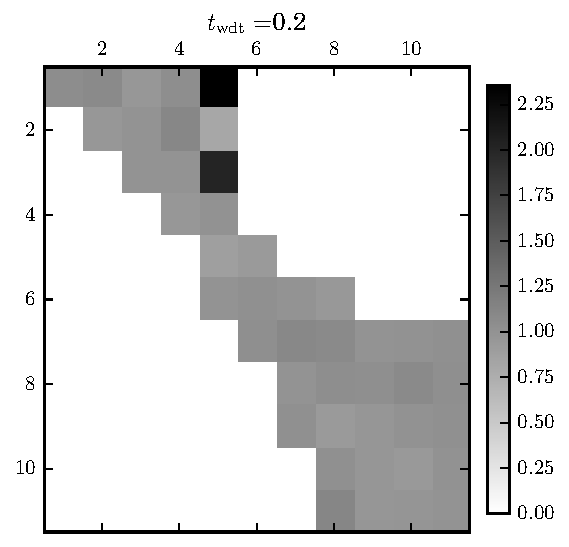
\includegraphics[scale=0.75]{images/results/matshows/homog_sp0_matshow_1}
    &
    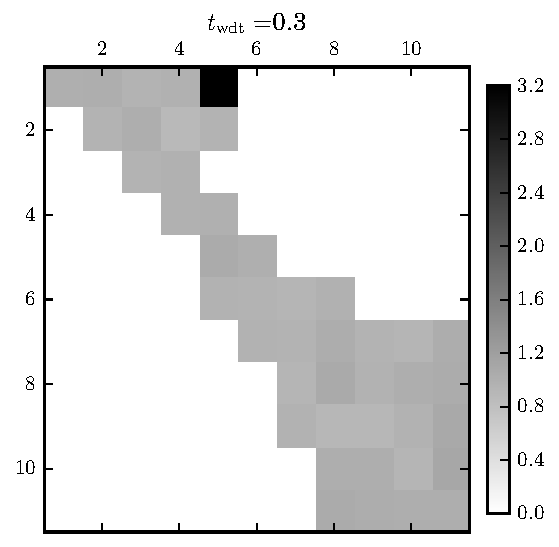
\includegraphics[scale=0.75]{images/results/matshows/homog_sp0_matshow_2}
    \\
    \input{include/tables/homog/matshows/homog_sp0_matshow_1} & \\
    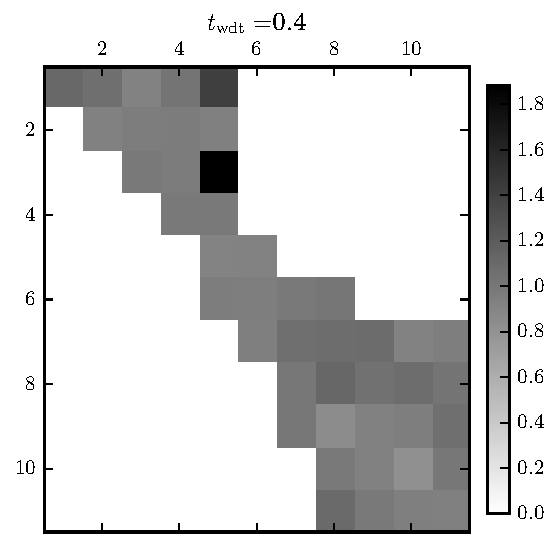
\includegraphics[scale=0.75]{images/results/matshows/homog_sp0_matshow_3}
    &
    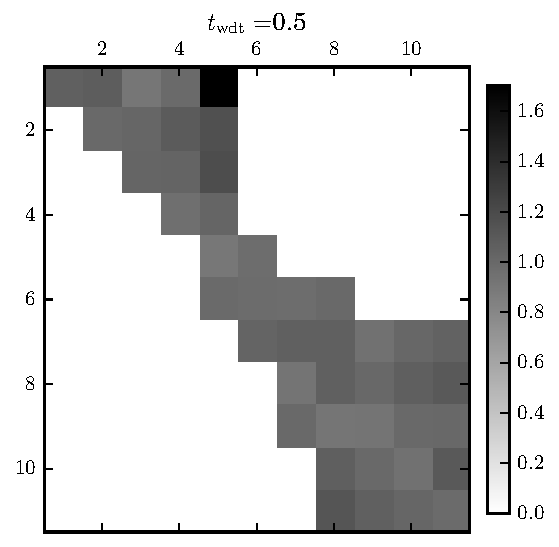
\includegraphics[scale=0.75]{images/results/matshows/homog_sp0_matshow_4}
    \\
    & \input{include/tables/homog/matshows/homog_sp0_matshow_4} \\
    \end{tabular}
\end{figure}

\begin{figure}[h]
  \centering
  \begin{tabular}{cccc}
    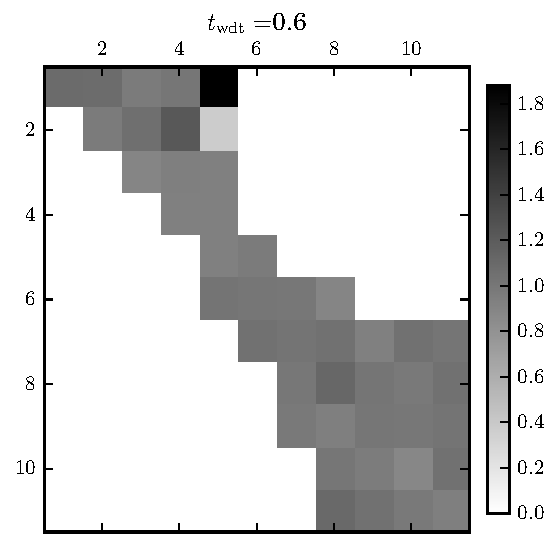
\includegraphics[scale=0.75]{images/results/matshows/homog_sp0_matshow_5}
    &
    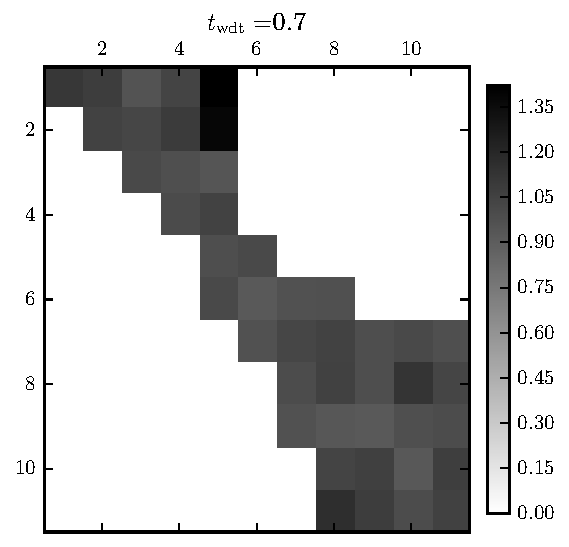
\includegraphics[scale=0.75]{images/results/matshows/homog_sp0_matshow_6}
    \\
&& \\
    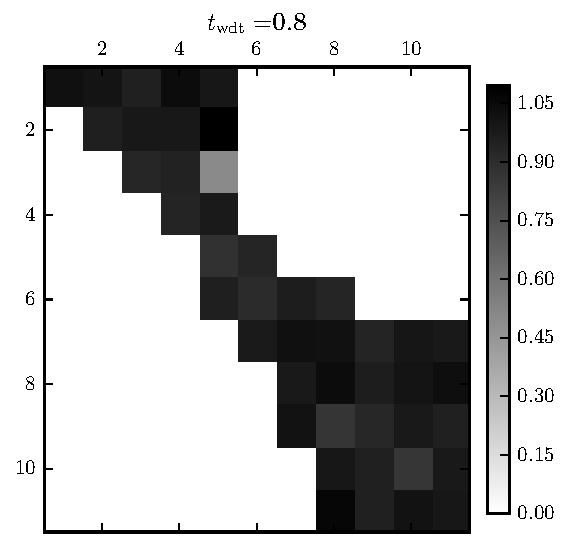
\includegraphics[scale=0.75]{images/results/matshows/homog_sp0_matshow_7}
    &
    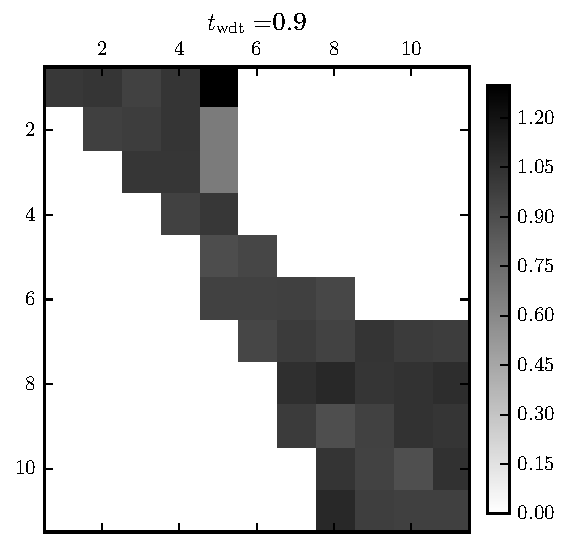
\includegraphics[scale=0.75]{images/results/matshows/homog_sp0_matshow_8}
    \\
    & \input{include/tables/homog/matshows/homog_sp0_matshow_8} \\
    \end{tabular}
\end{figure}

\begin{figure}[h]
  \centering
    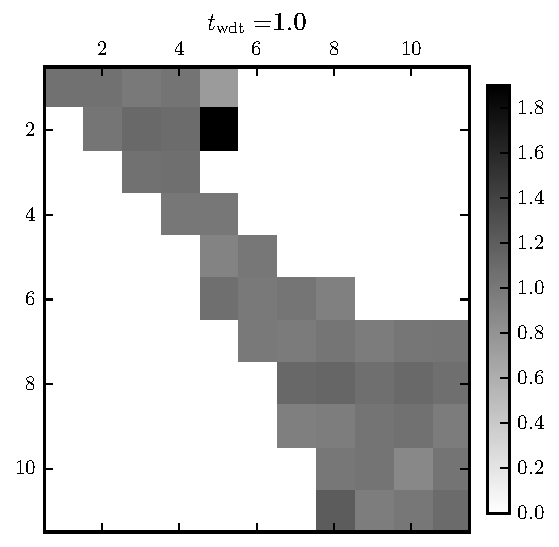
\includegraphics[scale=0.75]{images/results/matshows/homog_sp0_matshow_9}
\end{figure}

\newpage
\begin{landscape}
\subsection{Data}
\label{sec:homog_inf_sp0_raw}

\resizebox{1.2\textwidth}{!}{
\begin{tabular}{cccc}
  \spz{1}{1} & \spz{2}{1} & \spz{3}{1} & \spz{4}{1} \\
  \begin{tabular}{lrr}
\toprule
$t_{\mathrm{wdt}}$ & $\overline{\mathrm{FOM}}$ &    Ratio \\
\midrule
               0.1 &   2.303773$\times 10^{5}$ & 1.000000 \\
               0.2 &   2.416892$\times 10^{5}$ & 1.049102 \\
               0.3 &   2.307097$\times 10^{5}$ & 1.001443 \\
               0.4 &   2.564921$\times 10^{5}$ & 1.113356 \\
               0.5 &   2.444285$\times 10^{5}$ & 1.060992 \\
               0.6 &   2.490984$\times 10^{5}$ & 1.081263 \\
               0.7 &   2.534176$\times 10^{5}$ & 1.100011 \\
               0.8 &   2.355754$\times 10^{5}$ & 1.022563 \\
               0.9 &   2.311391$\times 10^{5}$ & 1.003307 \\
               1.0 &   2.407415$\times 10^{5}$ & 1.044988 \\
\bottomrule
\end{tabular}
 &
  \begin{tabular}{lrr}
\toprule
$t_{\mathrm{wdt}}$ & $\overline{\mathrm{FOM}}$ &    Ratio \\
\midrule
               0.1 &   4.683628$\times 10^{4}$ & 1.000000 \\
               0.2 &   5.021915$\times 10^{4}$ & 1.072228 \\
               0.3 &   4.771156$\times 10^{4}$ & 1.018688 \\
               0.4 &   4.989691$\times 10^{4}$ & 1.065348 \\
               0.5 &   5.067752$\times 10^{4}$ & 1.082014 \\
               0.6 &   5.026179$\times 10^{4}$ & 1.073138 \\
               0.7 &   5.050504$\times 10^{4}$ & 1.078332 \\
               0.8 &   4.699267$\times 10^{4}$ & 1.003339 \\
               0.9 &   4.816923$\times 10^{4}$ & 1.028460 \\
               1.0 &   4.888526$\times 10^{4}$ & 1.043748 \\
\bottomrule
\end{tabular}
 &
  \begin{tabular}{lrr}
\toprule
$t_{\mathrm{wdt}}$ & $\overline{\mathrm{FOM}}$ &    Ratio \\
\midrule
               0.1 &   6.204512$\times 10^{1}$ & 1.000000 \\
               0.2 &   5.950573$\times 10^{1}$ & 0.959072 \\
               0.3 &   5.956541$\times 10^{1}$ & 0.960034 \\
               0.4 &   5.722592$\times 10^{1}$ & 0.922328 \\
               0.5 &   5.680238$\times 10^{1}$ & 0.915501 \\
               0.6 &   6.048370$\times 10^{1}$ & 0.974834 \\
               0.7 &   5.914001$\times 10^{1}$ & 0.953177 \\
               0.8 &   5.938799$\times 10^{1}$ & 0.957174 \\
               0.9 &   6.005187$\times 10^{1}$ & 0.967874 \\
               1.0 &   6.208868$\times 10^{1}$ & 1.000702 \\
\bottomrule
\end{tabular}
 &
  \begin{tabular}{lrr}
\toprule
$t_{\mathrm{wdt}}$ & $\overline{\mathrm{FOM}}$ &    Ratio \\
\midrule
               0.1 &  1.805025$\times 10^{-1}$ & 1.000000 \\
               0.2 &  1.890662$\times 10^{-1}$ & 1.047443 \\
               0.3 &  1.766837$\times 10^{-1}$ & 0.978843 \\
               0.4 &  1.853607$\times 10^{-1}$ & 1.026915 \\
               0.5 &  1.785362$\times 10^{-1}$ & 0.989106 \\
               0.6 &  1.818917$\times 10^{-1}$ & 1.007696 \\
               0.7 &  1.876230$\times 10^{-1}$ & 1.039448 \\
               0.8 &  1.881331$\times 10^{-1}$ & 1.042274 \\
               0.9 &  1.854686$\times 10^{-1}$ & 1.027513 \\
               1.0 &  1.869678$\times 10^{-1}$ & 1.035818 \\
\bottomrule
\end{tabular}
 \\
  \spz{6}{1} & \spz{6}{1} & \spz{7}{1} & \spz{8}{1} \\
  \begin{tabular}{lrr}
\toprule
$t_{\mathrm{wdt}}$ & $\overline{\mathrm{FOM}}$ &    Ratio \\
\midrule
               0.1 &  7.577997$\times 10^{-4}$ & 1.000000 \\
               0.2 &  1.784195$\times 10^{-3}$ & 2.354441 \\
               0.3 &  2.426759$\times 10^{-3}$ & 3.202375 \\
               0.4 &  1.070218$\times 10^{-3}$ & 1.412270 \\
               0.5 &  1.290321$\times 10^{-3}$ & 1.702721 \\
               0.6 &  1.424939$\times 10^{-3}$ & 1.880364 \\
               0.7 &  1.076956$\times 10^{-3}$ & 1.421162 \\
               0.8 &  7.544624$\times 10^{-4}$ & 0.995596 \\
               0.9 &  9.838320$\times 10^{-4}$ & 1.298275 \\
               1.0 &  5.670118$\times 10^{-4}$ & 0.748234 \\
\bottomrule
\end{tabular}
 &
  \begin{tabular}{lrr}
\toprule
$t_{\mathrm{wdt}}$ & $\overline{\mathrm{FOM}}$ &    Ratio \\
\midrule
               0.1 &   0.000000$\times 10^{0}$ & 0.000000 \\
               0.2 &   0.000000$\times 10^{0}$ & 0.000000 \\
               0.3 &   0.000000$\times 10^{0}$ & 0.000000 \\
               0.4 &   0.000000$\times 10^{0}$ & 0.000000 \\
               0.5 &  3.679430$\times 10^{-4}$ & 0.000368 \\
               0.6 &   0.000000$\times 10^{0}$ & 0.000000 \\
               0.7 &   0.000000$\times 10^{0}$ & 0.000000 \\
               0.8 &   0.000000$\times 10^{0}$ & 0.000000 \\
               0.9 &   0.000000$\times 10^{0}$ & 0.000000 \\
               1.0 &   0.000000$\times 10^{0}$ & 0.000000 \\
\bottomrule
\end{tabular}
& 
  \begin{tabular}{lrr}
\toprule
$t_{\mathrm{wdt}}$ & $\overline{\mathrm{FOM}}$ &    Ratio \\
\midrule
               0.1 &   0.000000$\times 10^{0}$ & 0.000000 \\
               0.2 &   0.000000$\times 10^{0}$ & 0.000000 \\
               0.3 &   0.000000$\times 10^{0}$ & 0.000000 \\
               0.4 &   0.000000$\times 10^{0}$ & 0.000000 \\
               0.5 &   0.000000$\times 10^{0}$ & 0.000000 \\
               0.6 &   0.000000$\times 10^{0}$ & 0.000000 \\
               0.7 &   0.000000$\times 10^{0}$ & 0.000000 \\
               0.8 &   0.000000$\times 10^{0}$ & 0.000000 \\
               0.9 &   0.000000$\times 10^{0}$ & 0.000000 \\
               1.0 &   0.000000$\times 10^{0}$ & 0.000000 \\
\bottomrule
\end{tabular}
 &
  \begin{tabular}{lrr}
\toprule
$t_{\mathrm{wdt}}$ & $\overline{\mathrm{FOM}}$ &    Ratio \\
\midrule
               0.1 &   0.000000$\times 10^{0}$ & 0.000000 \\
               0.2 &   0.000000$\times 10^{0}$ & 0.000000 \\
               0.3 &   0.000000$\times 10^{0}$ & 0.000000 \\
               0.4 &   0.000000$\times 10^{0}$ & 0.000000 \\
               0.5 &   0.000000$\times 10^{0}$ & 0.000000 \\
               0.6 &   0.000000$\times 10^{0}$ & 0.000000 \\
               0.7 &   0.000000$\times 10^{0}$ & 0.000000 \\
               0.8 &   0.000000$\times 10^{0}$ & 0.000000 \\
               0.9 &   0.000000$\times 10^{0}$ & 0.000000 \\
               1.0 &   0.000000$\times 10^{0}$ & 0.000000 \\
\bottomrule
\end{tabular}
 \\
  \spz{9}{1} & \spz{10}{1} & \spz{11}{1} \\
  \begin{tabular}{lrr}
\toprule
$t_{\mathrm{wdt}}$ & $\overline{\mathrm{FOM}}$ &    Ratio \\
\midrule
               0.1 &   0.000000$\times 10^{0}$ & 0.000000 \\
               0.2 &   0.000000$\times 10^{0}$ & 0.000000 \\
               0.3 &   0.000000$\times 10^{0}$ & 0.000000 \\
               0.4 &   0.000000$\times 10^{0}$ & 0.000000 \\
               0.5 &   0.000000$\times 10^{0}$ & 0.000000 \\
               0.6 &   0.000000$\times 10^{0}$ & 0.000000 \\
               0.7 &   0.000000$\times 10^{0}$ & 0.000000 \\
               0.8 &   0.000000$\times 10^{0}$ & 0.000000 \\
               0.9 &   0.000000$\times 10^{0}$ & 0.000000 \\
               1.0 &   0.000000$\times 10^{0}$ & 0.000000 \\
\bottomrule
\end{tabular}
 &
  \begin{tabular}{lrr}
\toprule
$t_{\mathrm{wdt}}$ & $\overline{\mathrm{FOM}}$ &    Ratio \\
\midrule
               0.1 &   0.000000$\times 10^{0}$ & 0.000000 \\
               0.2 &   0.000000$\times 10^{0}$ & 0.000000 \\
               0.3 &   0.000000$\times 10^{0}$ & 0.000000 \\
               0.4 &   0.000000$\times 10^{0}$ & 0.000000 \\
               0.5 &   0.000000$\times 10^{0}$ & 0.000000 \\
               0.6 &   0.000000$\times 10^{0}$ & 0.000000 \\
               0.7 &   0.000000$\times 10^{0}$ & 0.000000 \\
               0.8 &   0.000000$\times 10^{0}$ & 0.000000 \\
               0.9 &   0.000000$\times 10^{0}$ & 0.000000 \\
               1.0 &   0.000000$\times 10^{0}$ & 0.000000 \\
\bottomrule
\end{tabular}
& 
  \begin{tabular}{lrr}
\toprule
$t_{\mathrm{wdt}}$ & $\overline{\mathrm{FOM}}$ &    Ratio \\
\midrule
               0.1 &   0.000000$\times 10^{0}$ & 0.000000 \\
               0.2 &   0.000000$\times 10^{0}$ & 0.000000 \\
               0.3 &   0.000000$\times 10^{0}$ & 0.000000 \\
               0.4 &   0.000000$\times 10^{0}$ & 0.000000 \\
               0.5 &   0.000000$\times 10^{0}$ & 0.000000 \\
               0.6 &   0.000000$\times 10^{0}$ & 0.000000 \\
               0.7 &   0.000000$\times 10^{0}$ & 0.000000 \\
               0.8 &   0.000000$\times 10^{0}$ & 0.000000 \\
               0.9 &   0.000000$\times 10^{0}$ & 0.000000 \\
               1.0 &   0.000000$\times 10^{0}$ & 0.000000 \\
\bottomrule
\end{tabular}
 \\
\end{tabular}
}
% Group 2
\newpage
\resizebox{1.2\textwidth}{!}{
\begin{tabular}{cccc}
  \spz{1}{2} & \spz{2}{2} & \spz{3}{2} & \spz{4}{2} \\
  \begin{tabular}{lrr}
\toprule
$t_{\mathrm{wdt}}$ & $\overline{\mathrm{FOM}}$ &    Ratio \\
\midrule
               0.1 &   0.000000$\times 10^{0}$ & 0.000000 \\
               0.2 &   0.000000$\times 10^{0}$ & 0.000000 \\
               0.3 &   0.000000$\times 10^{0}$ & 0.000000 \\
               0.4 &   0.000000$\times 10^{0}$ & 0.000000 \\
               0.5 &   0.000000$\times 10^{0}$ & 0.000000 \\
               0.6 &   0.000000$\times 10^{0}$ & 0.000000 \\
               0.7 &   0.000000$\times 10^{0}$ & 0.000000 \\
               0.8 &   0.000000$\times 10^{0}$ & 0.000000 \\
               0.9 &   0.000000$\times 10^{0}$ & 0.000000 \\
               1.0 &   0.000000$\times 10^{0}$ & 0.000000 \\
\bottomrule
\end{tabular}
 &
  \begin{tabular}{lrr}
\toprule
$t_{\mathrm{wdt}}$ & $\overline{\mathrm{FOM}}$ &    Ratio \\
\midrule
               0.1 &   1.816543$\times 10^{7}$ & 1.000000 \\
               0.2 &   1.742745$\times 10^{7}$ & 0.959374 \\
               0.3 &   1.737686$\times 10^{7}$ & 0.956589 \\
               0.4 &   1.683882$\times 10^{7}$ & 0.926971 \\
               0.5 &   1.812368$\times 10^{7}$ & 0.997701 \\
               0.6 &   1.771710$\times 10^{7}$ & 0.975320 \\
               0.7 &   1.898330$\times 10^{7}$ & 1.045023 \\
               0.8 &   1.748141$\times 10^{7}$ & 0.962345 \\
               0.9 &   1.762244$\times 10^{7}$ & 0.970109 \\
               1.0 &   1.863098$\times 10^{7}$ & 1.025628 \\
\bottomrule
\end{tabular}
 &
  \begin{tabular}{lrr}
\toprule
$t_{\mathrm{wdt}}$ & $\overline{\mathrm{FOM}}$ &    Ratio \\
\midrule
               0.1 &   1.195780$\times 10^{6}$ & 1.000000 \\
               0.2 &   1.182143$\times 10^{6}$ & 0.988596 \\
               0.3 &   1.214955$\times 10^{6}$ & 1.016036 \\
               0.4 &   1.149282$\times 10^{6}$ & 0.961115 \\
               0.5 &   1.220434$\times 10^{6}$ & 1.020618 \\
               0.6 &   1.264691$\times 10^{6}$ & 1.057629 \\
               0.7 &   1.232960$\times 10^{6}$ & 1.031093 \\
               0.8 &   1.185685$\times 10^{6}$ & 0.991558 \\
               0.9 &   1.181820$\times 10^{6}$ & 0.988326 \\
               1.0 &   1.328150$\times 10^{6}$ & 1.110698 \\
\bottomrule
\end{tabular}
 &
  \begin{tabular}{lrr}
\toprule
$t_{\mathrm{wdt}}$ & $\overline{\mathrm{FOM}}$ &    Ratio \\
\midrule
               0.1 &  6.724069$\times 10^{-2}$ & 1.000000 \\
               0.2 &  7.459400$\times 10^{-2}$ & 1.109358 \\
               0.3 &  5.924054$\times 10^{-2}$ & 0.881022 \\
               0.4 &  6.512928$\times 10^{-2}$ & 0.968599 \\
               0.5 &  7.338837$\times 10^{-2}$ & 1.091428 \\
               0.6 &  8.277739$\times 10^{-2}$ & 1.231061 \\
               0.7 &  7.345341$\times 10^{-2}$ & 1.092395 \\
               0.8 &  6.654432$\times 10^{-2}$ & 0.989644 \\
               0.9 &  6.900854$\times 10^{-2}$ & 1.026291 \\
               1.0 &  7.309238$\times 10^{-2}$ & 1.087026 \\
\bottomrule
\end{tabular}
 \\
  \spz{6}{2} & \spz{6}{2} & \spz{7}{2} & \spz{8}{2} \\
  \begin{tabular}{lrr}
\toprule
$t_{\mathrm{wdt}}$ & $\overline{\mathrm{FOM}}$ &    Ratio \\
\midrule
               0.1 &  1.898731$\times 10^{-3}$ & 1.000000 \\
               0.2 &  1.528499$\times 10^{-3}$ & 0.805011 \\
               0.3 &  1.818228$\times 10^{-3}$ & 0.957602 \\
               0.4 &  1.786127$\times 10^{-3}$ & 0.940695 \\
               0.5 &  2.215810$\times 10^{-3}$ & 1.166995 \\
               0.6 &  7.114902$\times 10^{-4}$ & 0.374719 \\
               0.7 &  2.625849$\times 10^{-3}$ & 1.382950 \\
               0.8 &  2.080112$\times 10^{-3}$ & 1.095528 \\
               0.9 &  1.279446$\times 10^{-3}$ & 0.673843 \\
               1.0 &  3.608836$\times 10^{-3}$ & 1.900657 \\
\bottomrule
\end{tabular}
 &
  \begin{tabular}{lrr}
\toprule
$t_{\mathrm{wdt}}$ & $\overline{\mathrm{FOM}}$ &    Ratio \\
\midrule
               0.1 &   0.000000$\times 10^{0}$ & 0.000000 \\
               0.2 &   0.000000$\times 10^{0}$ & 0.000000 \\
               0.3 &   0.000000$\times 10^{0}$ & 0.000000 \\
               0.4 &   0.000000$\times 10^{0}$ & 0.000000 \\
               0.5 &   0.000000$\times 10^{0}$ & 0.000000 \\
               0.6 &   0.000000$\times 10^{0}$ & 0.000000 \\
               0.7 &   0.000000$\times 10^{0}$ & 0.000000 \\
               0.8 &   0.000000$\times 10^{0}$ & 0.000000 \\
               0.9 &   0.000000$\times 10^{0}$ & 0.000000 \\
               1.0 &   0.000000$\times 10^{0}$ & 0.000000 \\
\bottomrule
\end{tabular}
& 
  \begin{tabular}{lrr}
\toprule
$t_{\mathrm{wdt}}$ & $\overline{\mathrm{FOM}}$ &    Ratio \\
\midrule
               0.1 &   0.000000$\times 10^{0}$ & 0.000000 \\
               0.2 &   0.000000$\times 10^{0}$ & 0.000000 \\
               0.3 &   0.000000$\times 10^{0}$ & 0.000000 \\
               0.4 &   0.000000$\times 10^{0}$ & 0.000000 \\
               0.5 &   0.000000$\times 10^{0}$ & 0.000000 \\
               0.6 &   0.000000$\times 10^{0}$ & 0.000000 \\
               0.7 &   0.000000$\times 10^{0}$ & 0.000000 \\
               0.8 &   0.000000$\times 10^{0}$ & 0.000000 \\
               0.9 &   0.000000$\times 10^{0}$ & 0.000000 \\
               1.0 &   0.000000$\times 10^{0}$ & 0.000000 \\
\bottomrule
\end{tabular}
 &
  \begin{tabular}{lrr}
\toprule
$t_{\mathrm{wdt}}$ & $\overline{\mathrm{FOM}}$ &    Ratio \\
\midrule
               0.1 &   0.000000$\times 10^{0}$ & 0.000000 \\
               0.2 &   0.000000$\times 10^{0}$ & 0.000000 \\
               0.3 &   0.000000$\times 10^{0}$ & 0.000000 \\
               0.4 &   0.000000$\times 10^{0}$ & 0.000000 \\
               0.5 &   0.000000$\times 10^{0}$ & 0.000000 \\
               0.6 &   0.000000$\times 10^{0}$ & 0.000000 \\
               0.7 &   0.000000$\times 10^{0}$ & 0.000000 \\
               0.8 &   0.000000$\times 10^{0}$ & 0.000000 \\
               0.9 &   0.000000$\times 10^{0}$ & 0.000000 \\
               1.0 &   0.000000$\times 10^{0}$ & 0.000000 \\
\bottomrule
\end{tabular}
 \\
  \spz{9}{2} & \spz{10}{2} & \spz{11}{2} \\
  \begin{tabular}{lrr}
\toprule
$t_{\mathrm{wdt}}$ & $\overline{\mathrm{FOM}}$ &    Ratio \\
\midrule
               0.1 &   0.000000$\times 10^{0}$ & 0.000000 \\
               0.2 &   0.000000$\times 10^{0}$ & 0.000000 \\
               0.3 &   0.000000$\times 10^{0}$ & 0.000000 \\
               0.4 &   0.000000$\times 10^{0}$ & 0.000000 \\
               0.5 &   0.000000$\times 10^{0}$ & 0.000000 \\
               0.6 &   0.000000$\times 10^{0}$ & 0.000000 \\
               0.7 &   0.000000$\times 10^{0}$ & 0.000000 \\
               0.8 &   0.000000$\times 10^{0}$ & 0.000000 \\
               0.9 &   0.000000$\times 10^{0}$ & 0.000000 \\
               1.0 &   0.000000$\times 10^{0}$ & 0.000000 \\
\bottomrule
\end{tabular}
 &
  \begin{tabular}{lrr}
\toprule
$t_{\mathrm{wdt}}$ & $\overline{\mathrm{FOM}}$ &    Ratio \\
\midrule
               0.1 &   0.000000$\times 10^{0}$ & 0.000000 \\
               0.2 &   0.000000$\times 10^{0}$ & 0.000000 \\
               0.3 &   0.000000$\times 10^{0}$ & 0.000000 \\
               0.4 &   0.000000$\times 10^{0}$ & 0.000000 \\
               0.5 &   0.000000$\times 10^{0}$ & 0.000000 \\
               0.6 &   0.000000$\times 10^{0}$ & 0.000000 \\
               0.7 &   0.000000$\times 10^{0}$ & 0.000000 \\
               0.8 &   0.000000$\times 10^{0}$ & 0.000000 \\
               0.9 &   0.000000$\times 10^{0}$ & 0.000000 \\
               1.0 &   0.000000$\times 10^{0}$ & 0.000000 \\
\bottomrule
\end{tabular}
& 
  \begin{tabular}{lrr}
\toprule
$t_{\mathrm{wdt}}$ & $\overline{\mathrm{FOM}}$ &    Ratio \\
\midrule
               0.1 &   0.000000$\times 10^{0}$ & 0.000000 \\
               0.2 &   0.000000$\times 10^{0}$ & 0.000000 \\
               0.3 &   0.000000$\times 10^{0}$ & 0.000000 \\
               0.4 &   0.000000$\times 10^{0}$ & 0.000000 \\
               0.5 &   0.000000$\times 10^{0}$ & 0.000000 \\
               0.6 &   0.000000$\times 10^{0}$ & 0.000000 \\
               0.7 &   0.000000$\times 10^{0}$ & 0.000000 \\
               0.8 &   0.000000$\times 10^{0}$ & 0.000000 \\
               0.9 &   0.000000$\times 10^{0}$ & 0.000000 \\
               1.0 &   0.000000$\times 10^{0}$ & 0.000000 \\
\bottomrule
\end{tabular}
 \\
\end{tabular}
}
% Group 3
\newpage
\resizebox{1.2\textwidth}{!}{
\begin{tabular}{cccc}
  \spz{1}{3} & \spz{2}{3} & \spz{3}{3} & \spz{4}{3} \\
  \begin{tabular}{lrr}
\toprule
$t_{\mathrm{wdt}}$ & $\overline{\mathrm{FOM}}$ &    Ratio \\
\midrule
               0.1 &   0.000000$\times 10^{0}$ & 0.000000 \\
               0.2 &   0.000000$\times 10^{0}$ & 0.000000 \\
               0.3 &   0.000000$\times 10^{0}$ & 0.000000 \\
               0.4 &   0.000000$\times 10^{0}$ & 0.000000 \\
               0.5 &   0.000000$\times 10^{0}$ & 0.000000 \\
               0.6 &   0.000000$\times 10^{0}$ & 0.000000 \\
               0.7 &   0.000000$\times 10^{0}$ & 0.000000 \\
               0.8 &   0.000000$\times 10^{0}$ & 0.000000 \\
               0.9 &   0.000000$\times 10^{0}$ & 0.000000 \\
               1.0 &   0.000000$\times 10^{0}$ & 0.000000 \\
\bottomrule
\end{tabular}
 &
  \begin{tabular}{lrr}
\toprule
$t_{\mathrm{wdt}}$ & $\overline{\mathrm{FOM}}$ &    Ratio \\
\midrule
               0.1 &   0.000000$\times 10^{0}$ & 0.000000 \\
               0.2 &   0.000000$\times 10^{0}$ & 0.000000 \\
               0.3 &   0.000000$\times 10^{0}$ & 0.000000 \\
               0.4 &   0.000000$\times 10^{0}$ & 0.000000 \\
               0.5 &   0.000000$\times 10^{0}$ & 0.000000 \\
               0.6 &   0.000000$\times 10^{0}$ & 0.000000 \\
               0.7 &   0.000000$\times 10^{0}$ & 0.000000 \\
               0.8 &   0.000000$\times 10^{0}$ & 0.000000 \\
               0.9 &   0.000000$\times 10^{0}$ & 0.000000 \\
               1.0 &   0.000000$\times 10^{0}$ & 0.000000 \\
\bottomrule
\end{tabular}
 &
  \begin{tabular}{lrr}
\toprule
$t_{\mathrm{wdt}}$ & $\overline{\mathrm{FOM}}$ &    Ratio \\
\midrule
               0.1 &   4.335975$\times 10^{9}$ & 1.000000 \\
               0.2 &   4.296860$\times 10^{9}$ & 0.990979 \\
               0.3 &   4.113044$\times 10^{9}$ & 0.948586 \\
               0.4 &   4.253757$\times 10^{9}$ & 0.981038 \\
               0.5 &   4.464645$\times 10^{9}$ & 1.029675 \\
               0.6 &   3.908586$\times 10^{9}$ & 0.901432 \\
               0.7 &   4.363567$\times 10^{9}$ & 1.006364 \\
               0.8 &   4.040146$\times 10^{9}$ & 0.931773 \\
               0.9 &   4.419446$\times 10^{9}$ & 1.019251 \\
               1.0 &   4.507271$\times 10^{9}$ & 1.039506 \\
\bottomrule
\end{tabular}
 &
  \begin{tabular}{lrr}
\toprule
$t_{\mathrm{wdt}}$ & $\overline{\mathrm{FOM}}$ &    Ratio \\
\midrule
               0.1 &   1.113999$\times 10^{7}$ & 1.000000 \\
               0.2 &   1.112852$\times 10^{7}$ & 0.998970 \\
               0.3 &   1.091167$\times 10^{7}$ & 0.979504 \\
               0.4 &   1.081007$\times 10^{7}$ & 0.970384 \\
               0.5 &   1.150492$\times 10^{7}$ & 1.032758 \\
               0.6 &   1.050764$\times 10^{7}$ & 0.943235 \\
               0.7 &   1.089186$\times 10^{7}$ & 0.977726 \\
               0.8 &   1.049502$\times 10^{7}$ & 0.942103 \\
               0.9 &   1.131167$\times 10^{7}$ & 1.015411 \\
               1.0 &   1.192004$\times 10^{7}$ & 1.070023 \\
\bottomrule
\end{tabular}
 \\
  \spz{6}{3} & \spz{6}{3} & \spz{7}{3} & \spz{8}{3} \\
  \begin{tabular}{lrr}
\toprule
$t_{\mathrm{wdt}}$ & $\overline{\mathrm{FOM}}$ &    Ratio \\
\midrule
               0.1 &  3.786882$\times 10^{-4}$ & 1.000000 \\
               0.2 &  7.631421$\times 10^{-4}$ & 2.015225 \\
               0.3 &   0.000000$\times 10^{0}$ & 0.000000 \\
               0.4 &  7.130278$\times 10^{-4}$ & 1.882889 \\
               0.5 &  4.501173$\times 10^{-4}$ & 1.188622 \\
               0.6 &  3.555212$\times 10^{-4}$ & 0.938823 \\
               0.7 &  3.585387$\times 10^{-4}$ & 0.946791 \\
               0.8 &  1.884120$\times 10^{-4}$ & 0.497539 \\
               0.9 &  2.554126$\times 10^{-4}$ & 0.674467 \\
               1.0 &   0.000000$\times 10^{0}$ & 0.000000 \\
\bottomrule
\end{tabular}
 &
  \begin{tabular}{lrr}
\toprule
$t_{\mathrm{wdt}}$ & $\overline{\mathrm{FOM}}$ &    Ratio \\
\midrule
               0.1 &   0.000000$\times 10^{0}$ & 0.000000 \\
               0.2 &   0.000000$\times 10^{0}$ & 0.000000 \\
               0.3 &   0.000000$\times 10^{0}$ & 0.000000 \\
               0.4 &   0.000000$\times 10^{0}$ & 0.000000 \\
               0.5 &   0.000000$\times 10^{0}$ & 0.000000 \\
               0.6 &   0.000000$\times 10^{0}$ & 0.000000 \\
               0.7 &   0.000000$\times 10^{0}$ & 0.000000 \\
               0.8 &   0.000000$\times 10^{0}$ & 0.000000 \\
               0.9 &   0.000000$\times 10^{0}$ & 0.000000 \\
               1.0 &   0.000000$\times 10^{0}$ & 0.000000 \\
\bottomrule
\end{tabular}
& 
  \begin{tabular}{lrr}
\toprule
$t_{\mathrm{wdt}}$ & $\overline{\mathrm{FOM}}$ &    Ratio \\
\midrule
               0.1 &   0.000000$\times 10^{0}$ & 0.000000 \\
               0.2 &   0.000000$\times 10^{0}$ & 0.000000 \\
               0.3 &   0.000000$\times 10^{0}$ & 0.000000 \\
               0.4 &   0.000000$\times 10^{0}$ & 0.000000 \\
               0.5 &   0.000000$\times 10^{0}$ & 0.000000 \\
               0.6 &   0.000000$\times 10^{0}$ & 0.000000 \\
               0.7 &   0.000000$\times 10^{0}$ & 0.000000 \\
               0.8 &   0.000000$\times 10^{0}$ & 0.000000 \\
               0.9 &   0.000000$\times 10^{0}$ & 0.000000 \\
               1.0 &   0.000000$\times 10^{0}$ & 0.000000 \\
\bottomrule
\end{tabular}
 &
  \begin{tabular}{lrr}
\toprule
$t_{\mathrm{wdt}}$ & $\overline{\mathrm{FOM}}$ &    Ratio \\
\midrule
               0.1 &   0.000000$\times 10^{0}$ & 0.000000 \\
               0.2 &   0.000000$\times 10^{0}$ & 0.000000 \\
               0.3 &   0.000000$\times 10^{0}$ & 0.000000 \\
               0.4 &   0.000000$\times 10^{0}$ & 0.000000 \\
               0.5 &   0.000000$\times 10^{0}$ & 0.000000 \\
               0.6 &   0.000000$\times 10^{0}$ & 0.000000 \\
               0.7 &   0.000000$\times 10^{0}$ & 0.000000 \\
               0.8 &   0.000000$\times 10^{0}$ & 0.000000 \\
               0.9 &   0.000000$\times 10^{0}$ & 0.000000 \\
               1.0 &   0.000000$\times 10^{0}$ & 0.000000 \\
\bottomrule
\end{tabular}
 \\
  \spz{9}{3} & \spz{10}{3} & \spz{11}{3} \\
  \begin{tabular}{lrr}
\toprule
$t_{\mathrm{wdt}}$ & $\overline{\mathrm{FOM}}$ &    Ratio \\
\midrule
               0.1 &   0.000000$\times 10^{0}$ & 0.000000 \\
               0.2 &   0.000000$\times 10^{0}$ & 0.000000 \\
               0.3 &   0.000000$\times 10^{0}$ & 0.000000 \\
               0.4 &   0.000000$\times 10^{0}$ & 0.000000 \\
               0.5 &   0.000000$\times 10^{0}$ & 0.000000 \\
               0.6 &   0.000000$\times 10^{0}$ & 0.000000 \\
               0.7 &   0.000000$\times 10^{0}$ & 0.000000 \\
               0.8 &   0.000000$\times 10^{0}$ & 0.000000 \\
               0.9 &   0.000000$\times 10^{0}$ & 0.000000 \\
               1.0 &   0.000000$\times 10^{0}$ & 0.000000 \\
\bottomrule
\end{tabular}
 &
  \begin{tabular}{lrr}
\toprule
$t_{\mathrm{wdt}}$ & $\overline{\mathrm{FOM}}$ &    Ratio \\
\midrule
               0.1 &   0.000000$\times 10^{0}$ & 0.000000 \\
               0.2 &   0.000000$\times 10^{0}$ & 0.000000 \\
               0.3 &   0.000000$\times 10^{0}$ & 0.000000 \\
               0.4 &   0.000000$\times 10^{0}$ & 0.000000 \\
               0.5 &   0.000000$\times 10^{0}$ & 0.000000 \\
               0.6 &   0.000000$\times 10^{0}$ & 0.000000 \\
               0.7 &   0.000000$\times 10^{0}$ & 0.000000 \\
               0.8 &   0.000000$\times 10^{0}$ & 0.000000 \\
               0.9 &   0.000000$\times 10^{0}$ & 0.000000 \\
               1.0 &   0.000000$\times 10^{0}$ & 0.000000 \\
\bottomrule
\end{tabular}
& 
  \begin{tabular}{lrr}
\toprule
$t_{\mathrm{wdt}}$ & $\overline{\mathrm{FOM}}$ &    Ratio \\
\midrule
               0.1 &   0.000000$\times 10^{0}$ & 0.000000 \\
               0.2 &   0.000000$\times 10^{0}$ & 0.000000 \\
               0.3 &   0.000000$\times 10^{0}$ & 0.000000 \\
               0.4 &   0.000000$\times 10^{0}$ & 0.000000 \\
               0.5 &   0.000000$\times 10^{0}$ & 0.000000 \\
               0.6 &   0.000000$\times 10^{0}$ & 0.000000 \\
               0.7 &   0.000000$\times 10^{0}$ & 0.000000 \\
               0.8 &   0.000000$\times 10^{0}$ & 0.000000 \\
               0.9 &   0.000000$\times 10^{0}$ & 0.000000 \\
               1.0 &   0.000000$\times 10^{0}$ & 0.000000 \\
\bottomrule
\end{tabular}
 \\
\end{tabular}
}

% Group 4
\newpage
\resizebox{1.2\textwidth}{!}{
\begin{tabular}{cccc}
  \spz{1}{4} & \spz{2}{4} & \spz{3}{4} & \spz{4}{4} \\
  \begin{tabular}{lrr}
\toprule
$t_{\mathrm{wdt}}$ & $\overline{\mathrm{FOM}}$ &    Ratio \\
\midrule
               0.1 &   0.000000$\times 10^{0}$ & 0.000000 \\
               0.2 &   0.000000$\times 10^{0}$ & 0.000000 \\
               0.3 &   0.000000$\times 10^{0}$ & 0.000000 \\
               0.4 &   0.000000$\times 10^{0}$ & 0.000000 \\
               0.5 &   0.000000$\times 10^{0}$ & 0.000000 \\
               0.6 &   0.000000$\times 10^{0}$ & 0.000000 \\
               0.7 &   0.000000$\times 10^{0}$ & 0.000000 \\
               0.8 &   0.000000$\times 10^{0}$ & 0.000000 \\
               0.9 &   0.000000$\times 10^{0}$ & 0.000000 \\
               1.0 &   0.000000$\times 10^{0}$ & 0.000000 \\
\bottomrule
\end{tabular}
 &
  \begin{tabular}{lrr}
\toprule
$t_{\mathrm{wdt}}$ & $\overline{\mathrm{FOM}}$ &    Ratio \\
\midrule
               0.1 &   0.000000$\times 10^{0}$ & 0.000000 \\
               0.2 &   0.000000$\times 10^{0}$ & 0.000000 \\
               0.3 &   0.000000$\times 10^{0}$ & 0.000000 \\
               0.4 &   0.000000$\times 10^{0}$ & 0.000000 \\
               0.5 &   0.000000$\times 10^{0}$ & 0.000000 \\
               0.6 &   0.000000$\times 10^{0}$ & 0.000000 \\
               0.7 &   0.000000$\times 10^{0}$ & 0.000000 \\
               0.8 &   0.000000$\times 10^{0}$ & 0.000000 \\
               0.9 &   0.000000$\times 10^{0}$ & 0.000000 \\
               1.0 &   0.000000$\times 10^{0}$ & 0.000000 \\
\bottomrule
\end{tabular}
 &
  \begin{tabular}{lrr}
\toprule
$t_{\mathrm{wdt}}$ & $\overline{\mathrm{FOM}}$ &    Ratio \\
\midrule
               0.1 &   0.000000$\times 10^{0}$ & 0.000000 \\
               0.2 &   0.000000$\times 10^{0}$ & 0.000000 \\
               0.3 &   0.000000$\times 10^{0}$ & 0.000000 \\
               0.4 &   0.000000$\times 10^{0}$ & 0.000000 \\
               0.5 &   0.000000$\times 10^{0}$ & 0.000000 \\
               0.6 &   0.000000$\times 10^{0}$ & 0.000000 \\
               0.7 &   0.000000$\times 10^{0}$ & 0.000000 \\
               0.8 &   0.000000$\times 10^{0}$ & 0.000000 \\
               0.9 &   0.000000$\times 10^{0}$ & 0.000000 \\
               1.0 &   0.000000$\times 10^{0}$ & 0.000000 \\
\bottomrule
\end{tabular}
 &
  \begin{tabular}{lrr}
\toprule
$t_{\mathrm{wdt}}$ & $\overline{\mathrm{FOM}}$ &    Ratio \\
\midrule
               0.1 &   4.050509$\times 10^{9}$ & 1.000000 \\
               0.2 &   3.882580$\times 10^{9}$ & 0.958541 \\
               0.3 &   3.983787$\times 10^{9}$ & 0.983528 \\
               0.4 &   4.016648$\times 10^{9}$ & 0.991640 \\
               0.5 &   3.900661$\times 10^{9}$ & 0.963005 \\
               0.6 &   3.792559$\times 10^{9}$ & 0.936317 \\
               0.7 &   4.062163$\times 10^{9}$ & 1.002877 \\
               0.8 &   3.812723$\times 10^{9}$ & 0.941295 \\
               0.9 &   3.915575$\times 10^{9}$ & 0.966687 \\
               1.0 &   4.087541$\times 10^{9}$ & 1.009143 \\
\bottomrule
\end{tabular}
 \\
  \spz{6}{4} & \spz{6}{4} & \spz{7}{4} & \spz{8}{4} \\
  \begin{tabular}{lrr}
\toprule
$t_{\mathrm{wdt}}$ & $\overline{\mathrm{FOM}}$ &    Ratio \\
\midrule
               0.1 &   9.074242$\times 10^{6}$ & 1.000000 \\
               0.2 &   9.164401$\times 10^{6}$ & 1.009936 \\
               0.3 &   8.978538$\times 10^{6}$ & 0.989453 \\
               0.4 &   9.002886$\times 10^{6}$ & 0.992136 \\
               0.5 &   9.352286$\times 10^{6}$ & 1.030641 \\
               0.6 &   8.471827$\times 10^{6}$ & 0.933613 \\
               0.7 &   9.488225$\times 10^{6}$ & 1.045622 \\
               0.8 &   8.862906$\times 10^{6}$ & 0.976710 \\
               0.9 &   9.167852$\times 10^{6}$ & 1.010316 \\
               1.0 &   9.217577$\times 10^{6}$ & 1.015796 \\
\bottomrule
\end{tabular}
 &
  \begin{tabular}{lrr}
\toprule
$t_{\mathrm{wdt}}$ & $\overline{\mathrm{FOM}}$ &    Ratio \\
\midrule
               0.1 &   0.000000$\times 10^{0}$ & 0.000000 \\
               0.2 &   0.000000$\times 10^{0}$ & 0.000000 \\
               0.3 &   0.000000$\times 10^{0}$ & 0.000000 \\
               0.4 &   0.000000$\times 10^{0}$ & 0.000000 \\
               0.5 &   0.000000$\times 10^{0}$ & 0.000000 \\
               0.6 &   0.000000$\times 10^{0}$ & 0.000000 \\
               0.7 &   0.000000$\times 10^{0}$ & 0.000000 \\
               0.8 &   0.000000$\times 10^{0}$ & 0.000000 \\
               0.9 &   0.000000$\times 10^{0}$ & 0.000000 \\
               1.0 &   0.000000$\times 10^{0}$ & 0.000000 \\
\bottomrule
\end{tabular}
& 
  \begin{tabular}{lrr}
\toprule
$t_{\mathrm{wdt}}$ & $\overline{\mathrm{FOM}}$ &    Ratio \\
\midrule
               0.1 &   0.000000$\times 10^{0}$ & 0.000000 \\
               0.2 &   0.000000$\times 10^{0}$ & 0.000000 \\
               0.3 &   0.000000$\times 10^{0}$ & 0.000000 \\
               0.4 &   0.000000$\times 10^{0}$ & 0.000000 \\
               0.5 &   0.000000$\times 10^{0}$ & 0.000000 \\
               0.6 &   0.000000$\times 10^{0}$ & 0.000000 \\
               0.7 &   0.000000$\times 10^{0}$ & 0.000000 \\
               0.8 &   0.000000$\times 10^{0}$ & 0.000000 \\
               0.9 &   0.000000$\times 10^{0}$ & 0.000000 \\
               1.0 &   0.000000$\times 10^{0}$ & 0.000000 \\
\bottomrule
\end{tabular}
 &
  \begin{tabular}{lrr}
\toprule
$t_{\mathrm{wdt}}$ & $\overline{\mathrm{FOM}}$ &    Ratio \\
\midrule
               0.1 &   0.000000$\times 10^{0}$ & 0.000000 \\
               0.2 &   0.000000$\times 10^{0}$ & 0.000000 \\
               0.3 &   0.000000$\times 10^{0}$ & 0.000000 \\
               0.4 &   0.000000$\times 10^{0}$ & 0.000000 \\
               0.5 &   0.000000$\times 10^{0}$ & 0.000000 \\
               0.6 &   0.000000$\times 10^{0}$ & 0.000000 \\
               0.7 &   0.000000$\times 10^{0}$ & 0.000000 \\
               0.8 &   0.000000$\times 10^{0}$ & 0.000000 \\
               0.9 &   0.000000$\times 10^{0}$ & 0.000000 \\
               1.0 &   0.000000$\times 10^{0}$ & 0.000000 \\
\bottomrule
\end{tabular}
 \\
  \spz{9}{4} & \spz{10}{4} & \spz{11}{4} \\
  \begin{tabular}{lrr}
\toprule
$t_{\mathrm{wdt}}$ & $\overline{\mathrm{FOM}}$ &    Ratio \\
\midrule
               0.1 &   0.000000$\times 10^{0}$ & 0.000000 \\
               0.2 &   0.000000$\times 10^{0}$ & 0.000000 \\
               0.3 &   0.000000$\times 10^{0}$ & 0.000000 \\
               0.4 &   0.000000$\times 10^{0}$ & 0.000000 \\
               0.5 &   0.000000$\times 10^{0}$ & 0.000000 \\
               0.6 &   0.000000$\times 10^{0}$ & 0.000000 \\
               0.7 &   0.000000$\times 10^{0}$ & 0.000000 \\
               0.8 &   0.000000$\times 10^{0}$ & 0.000000 \\
               0.9 &   0.000000$\times 10^{0}$ & 0.000000 \\
               1.0 &   0.000000$\times 10^{0}$ & 0.000000 \\
\bottomrule
\end{tabular}
 &
  \begin{tabular}{lrr}
\toprule
$t_{\mathrm{wdt}}$ & $\overline{\mathrm{FOM}}$ &    Ratio \\
\midrule
               0.1 &   0.000000$\times 10^{0}$ & 0.000000 \\
               0.2 &   0.000000$\times 10^{0}$ & 0.000000 \\
               0.3 &   0.000000$\times 10^{0}$ & 0.000000 \\
               0.4 &   0.000000$\times 10^{0}$ & 0.000000 \\
               0.5 &   0.000000$\times 10^{0}$ & 0.000000 \\
               0.6 &   0.000000$\times 10^{0}$ & 0.000000 \\
               0.7 &   0.000000$\times 10^{0}$ & 0.000000 \\
               0.8 &   0.000000$\times 10^{0}$ & 0.000000 \\
               0.9 &   0.000000$\times 10^{0}$ & 0.000000 \\
               1.0 &   0.000000$\times 10^{0}$ & 0.000000 \\
\bottomrule
\end{tabular}
& 
  \begin{tabular}{lrr}
\toprule
$t_{\mathrm{wdt}}$ & $\overline{\mathrm{FOM}}$ &    Ratio \\
\midrule
               0.1 &   0.000000$\times 10^{0}$ & 0.000000 \\
               0.2 &   0.000000$\times 10^{0}$ & 0.000000 \\
               0.3 &   0.000000$\times 10^{0}$ & 0.000000 \\
               0.4 &   0.000000$\times 10^{0}$ & 0.000000 \\
               0.5 &   0.000000$\times 10^{0}$ & 0.000000 \\
               0.6 &   0.000000$\times 10^{0}$ & 0.000000 \\
               0.7 &   0.000000$\times 10^{0}$ & 0.000000 \\
               0.8 &   0.000000$\times 10^{0}$ & 0.000000 \\
               0.9 &   0.000000$\times 10^{0}$ & 0.000000 \\
               1.0 &   0.000000$\times 10^{0}$ & 0.000000 \\
\bottomrule
\end{tabular}
 \\
\end{tabular}
}
% Group 5
\newpage
\resizebox{1.2\textwidth}{!}{
\begin{tabular}{cccc}
  \spz{1}{5} & \spz{2}{5} & \spz{3}{5} & \spz{4}{5} \\
  \begin{tabular}{lrr}
\toprule
$t_{\mathrm{wdt}}$ & $\overline{\mathrm{FOM}}$ &    Ratio \\
\midrule
               0.1 &   0.000000$\times 10^{0}$ & 0.000000 \\
               0.2 &   0.000000$\times 10^{0}$ & 0.000000 \\
               0.3 &   0.000000$\times 10^{0}$ & 0.000000 \\
               0.4 &   0.000000$\times 10^{0}$ & 0.000000 \\
               0.5 &   0.000000$\times 10^{0}$ & 0.000000 \\
               0.6 &   0.000000$\times 10^{0}$ & 0.000000 \\
               0.7 &   0.000000$\times 10^{0}$ & 0.000000 \\
               0.8 &   0.000000$\times 10^{0}$ & 0.000000 \\
               0.9 &   0.000000$\times 10^{0}$ & 0.000000 \\
               1.0 &   0.000000$\times 10^{0}$ & 0.000000 \\
\bottomrule
\end{tabular}
 &
  \begin{tabular}{lrr}
\toprule
$t_{\mathrm{wdt}}$ & $\overline{\mathrm{FOM}}$ &    Ratio \\
\midrule
               0.1 &   0.000000$\times 10^{0}$ & 0.000000 \\
               0.2 &   0.000000$\times 10^{0}$ & 0.000000 \\
               0.3 &   0.000000$\times 10^{0}$ & 0.000000 \\
               0.4 &   0.000000$\times 10^{0}$ & 0.000000 \\
               0.5 &   0.000000$\times 10^{0}$ & 0.000000 \\
               0.6 &   0.000000$\times 10^{0}$ & 0.000000 \\
               0.7 &   0.000000$\times 10^{0}$ & 0.000000 \\
               0.8 &   0.000000$\times 10^{0}$ & 0.000000 \\
               0.9 &   0.000000$\times 10^{0}$ & 0.000000 \\
               1.0 &   0.000000$\times 10^{0}$ & 0.000000 \\
\bottomrule
\end{tabular}
 &
  \begin{tabular}{lrr}
\toprule
$t_{\mathrm{wdt}}$ & $\overline{\mathrm{FOM}}$ &    Ratio \\
\midrule
               0.1 &   0.000000$\times 10^{0}$ & 0.000000 \\
               0.2 &   0.000000$\times 10^{0}$ & 0.000000 \\
               0.3 &   0.000000$\times 10^{0}$ & 0.000000 \\
               0.4 &   0.000000$\times 10^{0}$ & 0.000000 \\
               0.5 &   0.000000$\times 10^{0}$ & 0.000000 \\
               0.6 &   0.000000$\times 10^{0}$ & 0.000000 \\
               0.7 &   0.000000$\times 10^{0}$ & 0.000000 \\
               0.8 &   0.000000$\times 10^{0}$ & 0.000000 \\
               0.9 &   0.000000$\times 10^{0}$ & 0.000000 \\
               1.0 &   0.000000$\times 10^{0}$ & 0.000000 \\
\bottomrule
\end{tabular}
 &
  \begin{tabular}{lrr}
\toprule
$t_{\mathrm{wdt}}$ & $\overline{\mathrm{FOM}}$ &    Ratio \\
\midrule
               0.1 &   0.000000$\times 10^{0}$ & 0.000000 \\
               0.2 &   0.000000$\times 10^{0}$ & 0.000000 \\
               0.3 &   0.000000$\times 10^{0}$ & 0.000000 \\
               0.4 &   0.000000$\times 10^{0}$ & 0.000000 \\
               0.5 &   0.000000$\times 10^{0}$ & 0.000000 \\
               0.6 &   0.000000$\times 10^{0}$ & 0.000000 \\
               0.7 &   0.000000$\times 10^{0}$ & 0.000000 \\
               0.8 &   0.000000$\times 10^{0}$ & 0.000000 \\
               0.9 &   0.000000$\times 10^{0}$ & 0.000000 \\
               1.0 &   0.000000$\times 10^{0}$ & 0.000000 \\
\bottomrule
\end{tabular}
 \\
  \spz{6}{5} & \spz{6}{5} & \spz{7}{5} & \spz{8}{5} \\
  \begin{tabular}{lrr}
\toprule
$t_{\mathrm{wdt}}$ & $\overline{\mathrm{FOM}}$ &    Ratio \\
\midrule
               0.1 &   2.107107$\times 10^{9}$ & 1.000000 \\
               0.2 &   1.874331$\times 10^{9}$ & 0.889528 \\
               0.3 &   2.216045$\times 10^{9}$ & 1.051700 \\
               0.4 &   1.910656$\times 10^{9}$ & 0.906768 \\
               0.5 &   1.916729$\times 10^{9}$ & 0.909650 \\
               0.6 &   1.979116$\times 10^{9}$ & 0.939258 \\
               0.7 &   2.074456$\times 10^{9}$ & 0.984505 \\
               0.8 &   1.856900$\times 10^{9}$ & 0.881256 \\
               0.9 &   1.910820$\times 10^{9}$ & 0.906845 \\
               1.0 &   1.925136$\times 10^{9}$ & 0.913640 \\
\bottomrule
\end{tabular}
 &
  \begin{tabular}{lrr}
\toprule
$t_{\mathrm{wdt}}$ & $\overline{\mathrm{FOM}}$ &    Ratio \\
\midrule
               0.1 &   5.809655$\times 10^{6}$ & 1.000000 \\
               0.2 &   5.418966$\times 10^{6}$ & 0.932752 \\
               0.3 &   5.825467$\times 10^{6}$ & 1.002722 \\
               0.4 &   5.357805$\times 10^{6}$ & 0.922224 \\
               0.5 &   5.633489$\times 10^{6}$ & 0.969677 \\
               0.6 &   5.634535$\times 10^{6}$ & 0.969857 \\
               0.7 &   5.875776$\times 10^{6}$ & 1.011381 \\
               0.8 &   5.424064$\times 10^{6}$ & 0.933629 \\
               0.9 &   5.457314$\times 10^{6}$ & 0.939352 \\
               1.0 &   5.893288$\times 10^{6}$ & 1.014396 \\
\bottomrule
\end{tabular}
& 
  \begin{tabular}{lrr}
\toprule
$t_{\mathrm{wdt}}$ & $\overline{\mathrm{FOM}}$ &    Ratio \\
\midrule
               0.1 &   0.000000$\times 10^{0}$ & 0.000000 \\
               0.2 &   0.000000$\times 10^{0}$ & 0.000000 \\
               0.3 &   0.000000$\times 10^{0}$ & 0.000000 \\
               0.4 &   0.000000$\times 10^{0}$ & 0.000000 \\
               0.5 &   0.000000$\times 10^{0}$ & 0.000000 \\
               0.6 &   0.000000$\times 10^{0}$ & 0.000000 \\
               0.7 &   0.000000$\times 10^{0}$ & 0.000000 \\
               0.8 &   0.000000$\times 10^{0}$ & 0.000000 \\
               0.9 &   0.000000$\times 10^{0}$ & 0.000000 \\
               1.0 &   0.000000$\times 10^{0}$ & 0.000000 \\
\bottomrule
\end{tabular}
 &
  \begin{tabular}{lrr}
\toprule
$t_{\mathrm{wdt}}$ & $\overline{\mathrm{FOM}}$ &    Ratio \\
\midrule
               0.1 &   0.000000$\times 10^{0}$ & 0.000000 \\
               0.2 &   0.000000$\times 10^{0}$ & 0.000000 \\
               0.3 &   0.000000$\times 10^{0}$ & 0.000000 \\
               0.4 &   0.000000$\times 10^{0}$ & 0.000000 \\
               0.5 &   0.000000$\times 10^{0}$ & 0.000000 \\
               0.6 &   0.000000$\times 10^{0}$ & 0.000000 \\
               0.7 &   0.000000$\times 10^{0}$ & 0.000000 \\
               0.8 &   0.000000$\times 10^{0}$ & 0.000000 \\
               0.9 &   0.000000$\times 10^{0}$ & 0.000000 \\
               1.0 &   0.000000$\times 10^{0}$ & 0.000000 \\
\bottomrule
\end{tabular}
 \\
  \spz{9}{5} & \spz{10}{5} & \spz{11}{5} \\
  \begin{tabular}{lrr}
\toprule
$t_{\mathrm{wdt}}$ & $\overline{\mathrm{FOM}}$ &    Ratio \\
\midrule
               0.1 &   0.000000$\times 10^{0}$ & 0.000000 \\
               0.2 &   0.000000$\times 10^{0}$ & 0.000000 \\
               0.3 &   0.000000$\times 10^{0}$ & 0.000000 \\
               0.4 &   0.000000$\times 10^{0}$ & 0.000000 \\
               0.5 &   0.000000$\times 10^{0}$ & 0.000000 \\
               0.6 &   0.000000$\times 10^{0}$ & 0.000000 \\
               0.7 &   0.000000$\times 10^{0}$ & 0.000000 \\
               0.8 &   0.000000$\times 10^{0}$ & 0.000000 \\
               0.9 &   0.000000$\times 10^{0}$ & 0.000000 \\
               1.0 &   0.000000$\times 10^{0}$ & 0.000000 \\
\bottomrule
\end{tabular}
 &
  \begin{tabular}{lrr}
\toprule
$t_{\mathrm{wdt}}$ & $\overline{\mathrm{FOM}}$ &    Ratio \\
\midrule
               0.1 &   0.000000$\times 10^{0}$ & 0.000000 \\
               0.2 &   0.000000$\times 10^{0}$ & 0.000000 \\
               0.3 &   0.000000$\times 10^{0}$ & 0.000000 \\
               0.4 &   0.000000$\times 10^{0}$ & 0.000000 \\
               0.5 &   0.000000$\times 10^{0}$ & 0.000000 \\
               0.6 &   0.000000$\times 10^{0}$ & 0.000000 \\
               0.7 &   0.000000$\times 10^{0}$ & 0.000000 \\
               0.8 &   0.000000$\times 10^{0}$ & 0.000000 \\
               0.9 &   0.000000$\times 10^{0}$ & 0.000000 \\
               1.0 &   0.000000$\times 10^{0}$ & 0.000000 \\
\bottomrule
\end{tabular}
& 
  \begin{tabular}{lrr}
\toprule
$t_{\mathrm{wdt}}$ & $\overline{\mathrm{FOM}}$ &    Ratio \\
\midrule
               0.1 &   0.000000$\times 10^{0}$ & 0.000000 \\
               0.2 &   0.000000$\times 10^{0}$ & 0.000000 \\
               0.3 &   0.000000$\times 10^{0}$ & 0.000000 \\
               0.4 &   0.000000$\times 10^{0}$ & 0.000000 \\
               0.5 &   0.000000$\times 10^{0}$ & 0.000000 \\
               0.6 &   0.000000$\times 10^{0}$ & 0.000000 \\
               0.7 &   0.000000$\times 10^{0}$ & 0.000000 \\
               0.8 &   0.000000$\times 10^{0}$ & 0.000000 \\
               0.9 &   0.000000$\times 10^{0}$ & 0.000000 \\
               1.0 &   0.000000$\times 10^{0}$ & 0.000000 \\
\bottomrule
\end{tabular}
 \\
\end{tabular}
}

% Group 6
\newpage
\resizebox{1.2\textwidth}{!}{
\begin{tabular}{cccc}
  \spz{1}{6} & \spz{2}{6} & \spz{3}{6} & \spz{4}{6} \\
  \begin{tabular}{lrr}
\toprule
$t_{\mathrm{wdt}}$ & $\overline{\mathrm{FOM}}$ &    Ratio \\
\midrule
               0.1 &   0.000000$\times 10^{0}$ & 0.000000 \\
               0.2 &   0.000000$\times 10^{0}$ & 0.000000 \\
               0.3 &   0.000000$\times 10^{0}$ & 0.000000 \\
               0.4 &   0.000000$\times 10^{0}$ & 0.000000 \\
               0.5 &   0.000000$\times 10^{0}$ & 0.000000 \\
               0.6 &   0.000000$\times 10^{0}$ & 0.000000 \\
               0.7 &   0.000000$\times 10^{0}$ & 0.000000 \\
               0.8 &   0.000000$\times 10^{0}$ & 0.000000 \\
               0.9 &   0.000000$\times 10^{0}$ & 0.000000 \\
               1.0 &   0.000000$\times 10^{0}$ & 0.000000 \\
\bottomrule
\end{tabular}
 &
  \begin{tabular}{lrr}
\toprule
$t_{\mathrm{wdt}}$ & $\overline{\mathrm{FOM}}$ &    Ratio \\
\midrule
               0.1 &   0.000000$\times 10^{0}$ & 0.000000 \\
               0.2 &   0.000000$\times 10^{0}$ & 0.000000 \\
               0.3 &   0.000000$\times 10^{0}$ & 0.000000 \\
               0.4 &   0.000000$\times 10^{0}$ & 0.000000 \\
               0.5 &   0.000000$\times 10^{0}$ & 0.000000 \\
               0.6 &   0.000000$\times 10^{0}$ & 0.000000 \\
               0.7 &   0.000000$\times 10^{0}$ & 0.000000 \\
               0.8 &   0.000000$\times 10^{0}$ & 0.000000 \\
               0.9 &   0.000000$\times 10^{0}$ & 0.000000 \\
               1.0 &   0.000000$\times 10^{0}$ & 0.000000 \\
\bottomrule
\end{tabular}
 &
  \begin{tabular}{lrr}
\toprule
$t_{\mathrm{wdt}}$ & $\overline{\mathrm{FOM}}$ &    Ratio \\
\midrule
               0.1 &   0.000000$\times 10^{0}$ & 0.000000 \\
               0.2 &   0.000000$\times 10^{0}$ & 0.000000 \\
               0.3 &   0.000000$\times 10^{0}$ & 0.000000 \\
               0.4 &   0.000000$\times 10^{0}$ & 0.000000 \\
               0.5 &   0.000000$\times 10^{0}$ & 0.000000 \\
               0.6 &   0.000000$\times 10^{0}$ & 0.000000 \\
               0.7 &   0.000000$\times 10^{0}$ & 0.000000 \\
               0.8 &   0.000000$\times 10^{0}$ & 0.000000 \\
               0.9 &   0.000000$\times 10^{0}$ & 0.000000 \\
               1.0 &   0.000000$\times 10^{0}$ & 0.000000 \\
\bottomrule
\end{tabular}
 &
  \begin{tabular}{lrr}
\toprule
$t_{\mathrm{wdt}}$ & $\overline{\mathrm{FOM}}$ &    Ratio \\
\midrule
               0.1 &   0.000000$\times 10^{0}$ & 0.000000 \\
               0.2 &   0.000000$\times 10^{0}$ & 0.000000 \\
               0.3 &   0.000000$\times 10^{0}$ & 0.000000 \\
               0.4 &   0.000000$\times 10^{0}$ & 0.000000 \\
               0.5 &   0.000000$\times 10^{0}$ & 0.000000 \\
               0.6 &   0.000000$\times 10^{0}$ & 0.000000 \\
               0.7 &   0.000000$\times 10^{0}$ & 0.000000 \\
               0.8 &   0.000000$\times 10^{0}$ & 0.000000 \\
               0.9 &   0.000000$\times 10^{0}$ & 0.000000 \\
               1.0 &   0.000000$\times 10^{0}$ & 0.000000 \\
\bottomrule
\end{tabular}
 \\
  \spz{6}{6} & \spz{6}{6} & \spz{7}{6} & \spz{8}{6} \\
  \begin{tabular}{lrr}
\toprule
$t_{\mathrm{wdt}}$ & $\overline{\mathrm{FOM}}$ &    Ratio \\
\midrule
               0.1 &   4.663388$\times 10^{1}$ & 1.000000 \\
               0.2 &   4.673177$\times 10^{1}$ & 1.002099 \\
               0.3 &   4.531992$\times 10^{1}$ & 0.971824 \\
               0.4 &   4.465980$\times 10^{1}$ & 0.957669 \\
               0.5 &   4.608270$\times 10^{1}$ & 0.988181 \\
               0.6 &   4.780163$\times 10^{1}$ & 1.025041 \\
               0.7 &   4.703466$\times 10^{1}$ & 1.008594 \\
               0.8 &   4.471416$\times 10^{1}$ & 0.958834 \\
               0.9 &   4.477786$\times 10^{1}$ & 0.960200 \\
               1.0 &   5.001117$\times 10^{1}$ & 1.072421 \\
\bottomrule
\end{tabular}
 &
  \begin{tabular}{lrr}
\toprule
$t_{\mathrm{wdt}}$ & $\overline{\mathrm{FOM}}$ &    Ratio \\
\midrule
               0.1 &   6.179493$\times 10^{8}$ & 1.000000 \\
               0.2 &   6.278734$\times 10^{8}$ & 1.016060 \\
               0.3 &   5.930937$\times 10^{8}$ & 0.959777 \\
               0.4 &   5.870792$\times 10^{8}$ & 0.950044 \\
               0.5 &   6.030585$\times 10^{8}$ & 0.975903 \\
               0.6 &   6.258569$\times 10^{8}$ & 1.012797 \\
               0.7 &   5.660424$\times 10^{8}$ & 0.916001 \\
               0.8 &   5.626295$\times 10^{8}$ & 0.910478 \\
               0.9 &   5.943561$\times 10^{8}$ & 0.961820 \\
               1.0 &   6.130523$\times 10^{8}$ & 0.992075 \\
\bottomrule
\end{tabular}
& 
  \begin{tabular}{lrr}
\toprule
$t_{\mathrm{wdt}}$ & $\overline{\mathrm{FOM}}$ &    Ratio \\
\midrule
               0.1 &   2.254637$\times 10^{6}$ & 1.000000 \\
               0.2 &   2.233131$\times 10^{6}$ & 0.990461 \\
               0.3 &   2.091016$\times 10^{6}$ & 0.927429 \\
               0.4 &   2.218305$\times 10^{6}$ & 0.983886 \\
               0.5 &   2.187737$\times 10^{6}$ & 0.970328 \\
               0.6 &   2.263148$\times 10^{6}$ & 1.003775 \\
               0.7 &   2.187028$\times 10^{6}$ & 0.970013 \\
               0.8 &   2.177552$\times 10^{6}$ & 0.965810 \\
               0.9 &   2.190486$\times 10^{6}$ & 0.971547 \\
               1.0 &   2.318412$\times 10^{6}$ & 1.028286 \\
\bottomrule
\end{tabular}
 &
  \begin{tabular}{lrr}
\toprule
$t_{\mathrm{wdt}}$ & $\overline{\mathrm{FOM}}$ &    Ratio \\
\midrule
               0.1 &   5.296726$\times 10^{2}$ & 1.000000 \\
               0.2 &   5.032829$\times 10^{2}$ & 0.950177 \\
               0.3 &   5.173327$\times 10^{2}$ & 0.976703 \\
               0.4 &   5.342590$\times 10^{2}$ & 1.008659 \\
               0.5 &   5.301566$\times 10^{2}$ & 1.000914 \\
               0.6 &   4.761283$\times 10^{2}$ & 0.898911 \\
               0.7 &   5.168753$\times 10^{2}$ & 0.975839 \\
               0.8 &   4.951345$\times 10^{2}$ & 0.934794 \\
               0.9 &   4.948002$\times 10^{2}$ & 0.934162 \\
               1.0 &   5.019859$\times 10^{2}$ & 0.947729 \\
\bottomrule
\end{tabular}
 \\
  \spz{9}{6} & \spz{10}{6} & \spz{11}{6} \\
  \begin{tabular}{lrr}
\toprule
$t_{\mathrm{wdt}}$ & $\overline{\mathrm{FOM}}$ &    Ratio \\
\midrule
               0.1 &   0.000000$\times 10^{0}$ & 0.000000 \\
               0.2 &   0.000000$\times 10^{0}$ & 0.000000 \\
               0.3 &   0.000000$\times 10^{0}$ & 0.000000 \\
               0.4 &   0.000000$\times 10^{0}$ & 0.000000 \\
               0.5 &   0.000000$\times 10^{0}$ & 0.000000 \\
               0.6 &   0.000000$\times 10^{0}$ & 0.000000 \\
               0.7 &   0.000000$\times 10^{0}$ & 0.000000 \\
               0.8 &   0.000000$\times 10^{0}$ & 0.000000 \\
               0.9 &   0.000000$\times 10^{0}$ & 0.000000 \\
               1.0 &   0.000000$\times 10^{0}$ & 0.000000 \\
\bottomrule
\end{tabular}
 &
  \begin{tabular}{lrr}
\toprule
$t_{\mathrm{wdt}}$ & $\overline{\mathrm{FOM}}$ &    Ratio \\
\midrule
               0.1 &   0.000000$\times 10^{0}$ & 0.000000 \\
               0.2 &   0.000000$\times 10^{0}$ & 0.000000 \\
               0.3 &   0.000000$\times 10^{0}$ & 0.000000 \\
               0.4 &   0.000000$\times 10^{0}$ & 0.000000 \\
               0.5 &   0.000000$\times 10^{0}$ & 0.000000 \\
               0.6 &   0.000000$\times 10^{0}$ & 0.000000 \\
               0.7 &   0.000000$\times 10^{0}$ & 0.000000 \\
               0.8 &   0.000000$\times 10^{0}$ & 0.000000 \\
               0.9 &   0.000000$\times 10^{0}$ & 0.000000 \\
               1.0 &   0.000000$\times 10^{0}$ & 0.000000 \\
\bottomrule
\end{tabular}
& 
  \begin{tabular}{lrr}
\toprule
$t_{\mathrm{wdt}}$ & $\overline{\mathrm{FOM}}$ &    Ratio \\
\midrule
               0.1 &   0.000000$\times 10^{0}$ & 0.000000 \\
               0.2 &   0.000000$\times 10^{0}$ & 0.000000 \\
               0.3 &   0.000000$\times 10^{0}$ & 0.000000 \\
               0.4 &   0.000000$\times 10^{0}$ & 0.000000 \\
               0.5 &   0.000000$\times 10^{0}$ & 0.000000 \\
               0.6 &   0.000000$\times 10^{0}$ & 0.000000 \\
               0.7 &   0.000000$\times 10^{0}$ & 0.000000 \\
               0.8 &   0.000000$\times 10^{0}$ & 0.000000 \\
               0.9 &   0.000000$\times 10^{0}$ & 0.000000 \\
               1.0 &   0.000000$\times 10^{0}$ & 0.000000 \\
\bottomrule
\end{tabular}
 \\
\end{tabular}
}

% Group 7
\newpage
\resizebox{1.2\textwidth}{!}{
\begin{tabular}{cccc}
  \spz{1}{7} & \spz{2}{7} & \spz{3}{7} & \spz{4}{7} \\
  \begin{tabular}{lrr}
\toprule
$t_{\mathrm{wdt}}$ & $\overline{\mathrm{FOM}}$ &    Ratio \\
\midrule
               0.1 &   0.000000$\times 10^{0}$ & 0.000000 \\
               0.2 &   0.000000$\times 10^{0}$ & 0.000000 \\
               0.3 &   0.000000$\times 10^{0}$ & 0.000000 \\
               0.4 &   0.000000$\times 10^{0}$ & 0.000000 \\
               0.5 &   0.000000$\times 10^{0}$ & 0.000000 \\
               0.6 &   0.000000$\times 10^{0}$ & 0.000000 \\
               0.7 &   0.000000$\times 10^{0}$ & 0.000000 \\
               0.8 &   0.000000$\times 10^{0}$ & 0.000000 \\
               0.9 &   0.000000$\times 10^{0}$ & 0.000000 \\
               1.0 &   0.000000$\times 10^{0}$ & 0.000000 \\
\bottomrule
\end{tabular}
 &
  \begin{tabular}{lrr}
\toprule
$t_{\mathrm{wdt}}$ & $\overline{\mathrm{FOM}}$ &    Ratio \\
\midrule
               0.1 &   0.000000$\times 10^{0}$ & 0.000000 \\
               0.2 &   0.000000$\times 10^{0}$ & 0.000000 \\
               0.3 &   0.000000$\times 10^{0}$ & 0.000000 \\
               0.4 &   0.000000$\times 10^{0}$ & 0.000000 \\
               0.5 &   0.000000$\times 10^{0}$ & 0.000000 \\
               0.6 &   0.000000$\times 10^{0}$ & 0.000000 \\
               0.7 &   0.000000$\times 10^{0}$ & 0.000000 \\
               0.8 &   0.000000$\times 10^{0}$ & 0.000000 \\
               0.9 &   0.000000$\times 10^{0}$ & 0.000000 \\
               1.0 &   0.000000$\times 10^{0}$ & 0.000000 \\
\bottomrule
\end{tabular}
 &
  \begin{tabular}{lrr}
\toprule
$t_{\mathrm{wdt}}$ & $\overline{\mathrm{FOM}}$ &    Ratio \\
\midrule
               0.1 &   0.000000$\times 10^{0}$ & 0.000000 \\
               0.2 &   0.000000$\times 10^{0}$ & 0.000000 \\
               0.3 &   0.000000$\times 10^{0}$ & 0.000000 \\
               0.4 &   0.000000$\times 10^{0}$ & 0.000000 \\
               0.5 &   0.000000$\times 10^{0}$ & 0.000000 \\
               0.6 &   0.000000$\times 10^{0}$ & 0.000000 \\
               0.7 &   0.000000$\times 10^{0}$ & 0.000000 \\
               0.8 &   0.000000$\times 10^{0}$ & 0.000000 \\
               0.9 &   0.000000$\times 10^{0}$ & 0.000000 \\
               1.0 &   0.000000$\times 10^{0}$ & 0.000000 \\
\bottomrule
\end{tabular}
 &
  \begin{tabular}{lrr}
\toprule
$t_{\mathrm{wdt}}$ & $\overline{\mathrm{FOM}}$ &    Ratio \\
\midrule
               0.1 &   0.000000$\times 10^{0}$ & 0.000000 \\
               0.2 &   0.000000$\times 10^{0}$ & 0.000000 \\
               0.3 &   0.000000$\times 10^{0}$ & 0.000000 \\
               0.4 &   0.000000$\times 10^{0}$ & 0.000000 \\
               0.5 &   0.000000$\times 10^{0}$ & 0.000000 \\
               0.6 &   0.000000$\times 10^{0}$ & 0.000000 \\
               0.7 &   0.000000$\times 10^{0}$ & 0.000000 \\
               0.8 &   0.000000$\times 10^{0}$ & 0.000000 \\
               0.9 &   0.000000$\times 10^{0}$ & 0.000000 \\
               1.0 &   0.000000$\times 10^{0}$ & 0.000000 \\
\bottomrule
\end{tabular}
 \\
  \spz{6}{7} & \spz{6}{7} & \spz{7}{7} & \spz{8}{7} \\
  \begin{tabular}{lrr}
\toprule
$t_{\mathrm{wdt}}$ & $\overline{\mathrm{FOM}}$ &    Ratio \\
\midrule
               0.1 &   0.000000$\times 10^{0}$ & 0.000000 \\
               0.2 &   0.000000$\times 10^{0}$ & 0.000000 \\
               0.3 &   0.000000$\times 10^{0}$ & 0.000000 \\
               0.4 &   0.000000$\times 10^{0}$ & 0.000000 \\
               0.5 &   0.000000$\times 10^{0}$ & 0.000000 \\
               0.6 &   0.000000$\times 10^{0}$ & 0.000000 \\
               0.7 &   0.000000$\times 10^{0}$ & 0.000000 \\
               0.8 &   0.000000$\times 10^{0}$ & 0.000000 \\
               0.9 &   0.000000$\times 10^{0}$ & 0.000000 \\
               1.0 &   0.000000$\times 10^{0}$ & 0.000000 \\
\bottomrule
\end{tabular}
 &
  \begin{tabular}{lrr}
\toprule
$t_{\mathrm{wdt}}$ & $\overline{\mathrm{FOM}}$ &    Ratio \\
\midrule
               0.1 &   6.284840$\times 10^{3}$ & 1.000000 \\
               0.2 &   6.489712$\times 10^{3}$ & 1.032598 \\
               0.3 &   6.084867$\times 10^{3}$ & 0.968182 \\
               0.4 &   5.959359$\times 10^{3}$ & 0.948212 \\
               0.5 &   6.506662$\times 10^{3}$ & 1.035295 \\
               0.6 &   6.596779$\times 10^{3}$ & 1.049633 \\
               0.7 &   6.002478$\times 10^{3}$ & 0.955073 \\
               0.8 &   6.156212$\times 10^{3}$ & 0.979534 \\
               0.9 &   5.911256$\times 10^{3}$ & 0.940558 \\
               1.0 &   6.216781$\times 10^{3}$ & 0.989171 \\
\bottomrule
\end{tabular}
& 
  \begin{tabular}{lrr}
\toprule
$t_{\mathrm{wdt}}$ & $\overline{\mathrm{FOM}}$ &    Ratio \\
\midrule
               0.1 &   2.564454$\times 10^{7}$ & 1.000000 \\
               0.2 &   2.822263$\times 10^{7}$ & 1.100532 \\
               0.3 &   2.454385$\times 10^{7}$ & 0.957079 \\
               0.4 &   2.722732$\times 10^{7}$ & 1.061720 \\
               0.5 &   2.703728$\times 10^{7}$ & 1.054310 \\
               0.6 &   2.621164$\times 10^{7}$ & 1.022114 \\
               0.7 &   2.639073$\times 10^{7}$ & 1.029098 \\
               0.8 &   2.621284$\times 10^{7}$ & 1.022161 \\
               0.9 &   2.538075$\times 10^{7}$ & 0.989714 \\
               1.0 &   2.529530$\times 10^{7}$ & 0.986382 \\
\bottomrule
\end{tabular}
 &
  \begin{tabular}{lrr}
\toprule
$t_{\mathrm{wdt}}$ & $\overline{\mathrm{FOM}}$ &    Ratio \\
\midrule
               0.1 &   3.928172$\times 10^{5}$ & 1.000000 \\
               0.2 &   4.246792$\times 10^{5}$ & 1.081111 \\
               0.3 &   4.067453$\times 10^{5}$ & 1.035457 \\
               0.4 &   4.200058$\times 10^{5}$ & 1.069214 \\
               0.5 &   4.122694$\times 10^{5}$ & 1.049520 \\
               0.6 &   4.086363$\times 10^{5}$ & 1.040271 \\
               0.7 &   4.099811$\times 10^{5}$ & 1.043694 \\
               0.8 &   4.000836$\times 10^{5}$ & 1.018498 \\
               0.9 &   3.759083$\times 10^{5}$ & 0.956955 \\
               1.0 &   4.028877$\times 10^{5}$ & 1.025637 \\
\bottomrule
\end{tabular}
 \\
  \spz{9}{7} & \spz{10}{7} & \spz{11}{7} \\
  \begin{tabular}{lrr}
\toprule
$t_{\mathrm{wdt}}$ & $\overline{\mathrm{FOM}}$ &    Ratio \\
\midrule
               0.1 &   1.008565$\times 10^{4}$ & 1.000000 \\
               0.2 &   1.006397$\times 10^{4}$ & 0.997850 \\
               0.3 &   9.706334$\times 10^{3}$ & 0.962391 \\
               0.4 &   1.086260$\times 10^{4}$ & 1.077036 \\
               0.5 &   9.521993$\times 10^{3}$ & 0.944113 \\
               0.6 &   9.439352$\times 10^{3}$ & 0.935919 \\
               0.7 &   9.959517$\times 10^{3}$ & 0.987494 \\
               0.8 &   9.476622$\times 10^{3}$ & 0.939614 \\
               0.9 &   1.041477$\times 10^{4}$ & 1.032632 \\
               1.0 &   9.883803$\times 10^{3}$ & 0.979987 \\
\bottomrule
\end{tabular}
 &
  \begin{tabular}{lrr}
\toprule
$t_{\mathrm{wdt}}$ & $\overline{\mathrm{FOM}}$ &    Ratio \\
\midrule
               0.1 &   4.367493$\times 10^{3}$ & 1.000000 \\
               0.2 &   4.412325$\times 10^{3}$ & 1.010265 \\
               0.3 &   4.086353$\times 10^{3}$ & 0.935629 \\
               0.4 &   4.033994$\times 10^{3}$ & 0.923641 \\
               0.5 &   4.419448$\times 10^{3}$ & 1.011896 \\
               0.6 &   4.495731$\times 10^{3}$ & 1.029362 \\
               0.7 &   4.395034$\times 10^{3}$ & 1.006306 \\
               0.8 &   4.363608$\times 10^{3}$ & 0.999110 \\
               0.9 &   4.319923$\times 10^{3}$ & 0.989108 \\
               1.0 &   4.458088$\times 10^{3}$ & 1.020743 \\
\bottomrule
\end{tabular}
& 
  \begin{tabular}{lrr}
\toprule
$t_{\mathrm{wdt}}$ & $\overline{\mathrm{FOM}}$ &    Ratio \\
\midrule
               0.1 &   4.673141$\times 10^{2}$ & 1.000000 \\
               0.2 &   4.749493$\times 10^{2}$ & 1.016339 \\
               0.3 &   4.838791$\times 10^{2}$ & 1.035447 \\
               0.4 &   4.447622$\times 10^{2}$ & 0.951741 \\
               0.5 &   4.869820$\times 10^{2}$ & 1.042087 \\
               0.6 &   4.752545$\times 10^{2}$ & 1.016991 \\
               0.7 &   4.583026$\times 10^{2}$ & 0.980716 \\
               0.8 &   4.587925$\times 10^{2}$ & 0.981765 \\
               0.9 &   4.608184$\times 10^{2}$ & 0.986100 \\
               1.0 &   4.795647$\times 10^{2}$ & 1.026215 \\
\bottomrule
\end{tabular}
 \\
\end{tabular}
}

% Group 8
\newpage
\resizebox{1.2\textwidth}{!}{
\begin{tabular}{cccc}
  \spz{1}{8} & \spz{2}{8} & \spz{3}{8} & \spz{4}{8} \\
  \begin{tabular}{lrr}
\toprule
$t_{\mathrm{wdt}}$ & $\overline{\mathrm{FOM}}$ &    Ratio \\
\midrule
               0.1 &   0.000000$\times 10^{0}$ & 0.000000 \\
               0.2 &   0.000000$\times 10^{0}$ & 0.000000 \\
               0.3 &   0.000000$\times 10^{0}$ & 0.000000 \\
               0.4 &   0.000000$\times 10^{0}$ & 0.000000 \\
               0.5 &   0.000000$\times 10^{0}$ & 0.000000 \\
               0.6 &   0.000000$\times 10^{0}$ & 0.000000 \\
               0.7 &   0.000000$\times 10^{0}$ & 0.000000 \\
               0.8 &   0.000000$\times 10^{0}$ & 0.000000 \\
               0.9 &   0.000000$\times 10^{0}$ & 0.000000 \\
               1.0 &   0.000000$\times 10^{0}$ & 0.000000 \\
\bottomrule
\end{tabular}
 &
  \begin{tabular}{lrr}
\toprule
$t_{\mathrm{wdt}}$ & $\overline{\mathrm{FOM}}$ &    Ratio \\
\midrule
               0.1 &   0.000000$\times 10^{0}$ & 0.000000 \\
               0.2 &   0.000000$\times 10^{0}$ & 0.000000 \\
               0.3 &   0.000000$\times 10^{0}$ & 0.000000 \\
               0.4 &   0.000000$\times 10^{0}$ & 0.000000 \\
               0.5 &   0.000000$\times 10^{0}$ & 0.000000 \\
               0.6 &   0.000000$\times 10^{0}$ & 0.000000 \\
               0.7 &   0.000000$\times 10^{0}$ & 0.000000 \\
               0.8 &   0.000000$\times 10^{0}$ & 0.000000 \\
               0.9 &   0.000000$\times 10^{0}$ & 0.000000 \\
               1.0 &   0.000000$\times 10^{0}$ & 0.000000 \\
\bottomrule
\end{tabular}
 &
  \begin{tabular}{lrr}
\toprule
$t_{\mathrm{wdt}}$ & $\overline{\mathrm{FOM}}$ &    Ratio \\
\midrule
               0.1 &   0.000000$\times 10^{0}$ & 0.000000 \\
               0.2 &   0.000000$\times 10^{0}$ & 0.000000 \\
               0.3 &   0.000000$\times 10^{0}$ & 0.000000 \\
               0.4 &   0.000000$\times 10^{0}$ & 0.000000 \\
               0.5 &   0.000000$\times 10^{0}$ & 0.000000 \\
               0.6 &   0.000000$\times 10^{0}$ & 0.000000 \\
               0.7 &   0.000000$\times 10^{0}$ & 0.000000 \\
               0.8 &   0.000000$\times 10^{0}$ & 0.000000 \\
               0.9 &   0.000000$\times 10^{0}$ & 0.000000 \\
               1.0 &   0.000000$\times 10^{0}$ & 0.000000 \\
\bottomrule
\end{tabular}
 &
  \begin{tabular}{lrr}
\toprule
$t_{\mathrm{wdt}}$ & $\overline{\mathrm{FOM}}$ &    Ratio \\
\midrule
               0.1 &   0.000000$\times 10^{0}$ & 0.000000 \\
               0.2 &   0.000000$\times 10^{0}$ & 0.000000 \\
               0.3 &   0.000000$\times 10^{0}$ & 0.000000 \\
               0.4 &   0.000000$\times 10^{0}$ & 0.000000 \\
               0.5 &   0.000000$\times 10^{0}$ & 0.000000 \\
               0.6 &   0.000000$\times 10^{0}$ & 0.000000 \\
               0.7 &   0.000000$\times 10^{0}$ & 0.000000 \\
               0.8 &   0.000000$\times 10^{0}$ & 0.000000 \\
               0.9 &   0.000000$\times 10^{0}$ & 0.000000 \\
               1.0 &   0.000000$\times 10^{0}$ & 0.000000 \\
\bottomrule
\end{tabular}
 \\
  \spz{6}{8} & \spz{6}{8} & \spz{7}{8} & \spz{8}{8} \\
  \begin{tabular}{lrr}
\toprule
$t_{\mathrm{wdt}}$ & $\overline{\mathrm{FOM}}$ &    Ratio \\
\midrule
               0.1 &   0.000000$\times 10^{0}$ & 0.000000 \\
               0.2 &   0.000000$\times 10^{0}$ & 0.000000 \\
               0.3 &   0.000000$\times 10^{0}$ & 0.000000 \\
               0.4 &   0.000000$\times 10^{0}$ & 0.000000 \\
               0.5 &   0.000000$\times 10^{0}$ & 0.000000 \\
               0.6 &   0.000000$\times 10^{0}$ & 0.000000 \\
               0.7 &   0.000000$\times 10^{0}$ & 0.000000 \\
               0.8 &   0.000000$\times 10^{0}$ & 0.000000 \\
               0.9 &   0.000000$\times 10^{0}$ & 0.000000 \\
               1.0 &   0.000000$\times 10^{0}$ & 0.000000 \\
\bottomrule
\end{tabular}
 &
  \begin{tabular}{lrr}
\toprule
$t_{\mathrm{wdt}}$ & $\overline{\mathrm{FOM}}$ &    Ratio \\
\midrule
               0.1 &   0.000000$\times 10^{0}$ & 0.000000 \\
               0.2 &   0.000000$\times 10^{0}$ & 0.000000 \\
               0.3 &   0.000000$\times 10^{0}$ & 0.000000 \\
               0.4 &   0.000000$\times 10^{0}$ & 0.000000 \\
               0.5 &   0.000000$\times 10^{0}$ & 0.000000 \\
               0.6 &   0.000000$\times 10^{0}$ & 0.000000 \\
               0.7 &   0.000000$\times 10^{0}$ & 0.000000 \\
               0.8 &   0.000000$\times 10^{0}$ & 0.000000 \\
               0.9 &   0.000000$\times 10^{0}$ & 0.000000 \\
               1.0 &   0.000000$\times 10^{0}$ & 0.000000 \\
\bottomrule
\end{tabular}
& 
  \begin{tabular}{lrr}
\toprule
$t_{\mathrm{wdt}}$ & $\overline{\mathrm{FOM}}$ &    Ratio \\
\midrule
               0.1 &   3.624801$\times 10^{4}$ & 1.000000 \\
               0.2 &   3.573846$\times 10^{4}$ & 0.985943 \\
               0.3 &   3.357317$\times 10^{4}$ & 0.926207 \\
               0.4 &   3.633781$\times 10^{4}$ & 1.002478 \\
               0.5 &   3.367926$\times 10^{4}$ & 0.929134 \\
               0.6 &   3.623861$\times 10^{4}$ & 0.999741 \\
               0.7 &   3.604944$\times 10^{4}$ & 0.994522 \\
               0.8 &   3.555720$\times 10^{4}$ & 0.980942 \\
               0.9 &   3.833569$\times 10^{4}$ & 1.057595 \\
               1.0 &   4.075120$\times 10^{4}$ & 1.124233 \\
\bottomrule
\end{tabular}
 &
  \begin{tabular}{lrr}
\toprule
$t_{\mathrm{wdt}}$ & $\overline{\mathrm{FOM}}$ &    Ratio \\
\midrule
               0.1 &   6.604787$\times 10^{7}$ & 1.000000 \\
               0.2 &   6.908472$\times 10^{7}$ & 1.045980 \\
               0.3 &   7.029599$\times 10^{7}$ & 1.064319 \\
               0.4 &   7.393059$\times 10^{7}$ & 1.119349 \\
               0.5 &   7.000481$\times 10^{7}$ & 1.059910 \\
               0.6 &   7.395961$\times 10^{7}$ & 1.119788 \\
               0.7 &   6.979038$\times 10^{7}$ & 1.056664 \\
               0.8 &   6.892649$\times 10^{7}$ & 1.043584 \\
               0.9 &   7.212280$\times 10^{7}$ & 1.091978 \\
               1.0 &   7.517225$\times 10^{7}$ & 1.138148 \\
\bottomrule
\end{tabular}
 \\
  \spz{9}{8} & \spz{10}{8} & \spz{11}{8} \\
  \begin{tabular}{lrr}
\toprule
$t_{\mathrm{wdt}}$ & $\overline{\mathrm{FOM}}$ &    Ratio \\
\midrule
               0.1 &   2.370219$\times 10^{5}$ & 1.000000 \\
               0.2 &   2.461415$\times 10^{5}$ & 1.038476 \\
               0.3 &   2.312383$\times 10^{5}$ & 0.975599 \\
               0.4 &   2.482154$\times 10^{5}$ & 1.047226 \\
               0.5 &   2.382993$\times 10^{5}$ & 1.005390 \\
               0.6 &   2.402796$\times 10^{5}$ & 1.013744 \\
               0.7 &   2.334855$\times 10^{5}$ & 0.985080 \\
               0.8 &   2.300443$\times 10^{5}$ & 0.970562 \\
               0.9 &   2.419326$\times 10^{5}$ & 1.020719 \\
               1.0 &   2.521705$\times 10^{5}$ & 1.063913 \\
\bottomrule
\end{tabular}
 &
  \begin{tabular}{lrr}
\toprule
$t_{\mathrm{wdt}}$ & $\overline{\mathrm{FOM}}$ &    Ratio \\
\midrule
               0.1 &   8.528104$\times 10^{4}$ & 1.000000 \\
               0.2 &   9.249724$\times 10^{4}$ & 1.084617 \\
               0.3 &   8.746691$\times 10^{4}$ & 1.025631 \\
               0.4 &   9.099322$\times 10^{4}$ & 1.066981 \\
               0.5 &   9.093714$\times 10^{4}$ & 1.066323 \\
               0.6 &   8.454517$\times 10^{4}$ & 0.991371 \\
               0.7 &   9.626479$\times 10^{4}$ & 1.128795 \\
               0.8 &   8.543830$\times 10^{4}$ & 1.001844 \\
               0.9 &   8.853355$\times 10^{4}$ & 1.038139 \\
               1.0 &   9.493499$\times 10^{4}$ & 1.113202 \\
\bottomrule
\end{tabular}
& 
  \begin{tabular}{lrr}
\toprule
$t_{\mathrm{wdt}}$ & $\overline{\mathrm{FOM}}$ &    Ratio \\
\midrule
               0.1 &   1.888873$\times 10^{4}$ & 1.000000 \\
               0.2 &   1.961373$\times 10^{4}$ & 1.038383 \\
               0.3 &   1.968962$\times 10^{4}$ & 1.042401 \\
               0.4 &   1.940867$\times 10^{4}$ & 1.027527 \\
               0.5 &   2.083910$\times 10^{4}$ & 1.103256 \\
               0.6 &   1.943130$\times 10^{4}$ & 1.028725 \\
               0.7 &   1.953164$\times 10^{4}$ & 1.034037 \\
               0.8 &   1.945977$\times 10^{4}$ & 1.030232 \\
               0.9 &   2.015811$\times 10^{4}$ & 1.067203 \\
               1.0 &   2.006323$\times 10^{4}$ & 1.062180 \\
\bottomrule
\end{tabular}
 \\
\end{tabular}
}
% Group 9
\newpage
\resizebox{1.2\textwidth}{!}{
\begin{tabular}{cccc}
  \spz{1}{9} & \spz{2}{9} & \spz{3}{9} & \spz{4}{9} \\
  \begin{tabular}{lrr}
\toprule
$t_{\mathrm{wdt}}$ & $\overline{\mathrm{FOM}}$ &    Ratio \\
\midrule
               0.1 &   0.000000$\times 10^{0}$ & 0.000000 \\
               0.2 &   0.000000$\times 10^{0}$ & 0.000000 \\
               0.3 &   0.000000$\times 10^{0}$ & 0.000000 \\
               0.4 &   0.000000$\times 10^{0}$ & 0.000000 \\
               0.5 &   0.000000$\times 10^{0}$ & 0.000000 \\
               0.6 &   0.000000$\times 10^{0}$ & 0.000000 \\
               0.7 &   0.000000$\times 10^{0}$ & 0.000000 \\
               0.8 &   0.000000$\times 10^{0}$ & 0.000000 \\
               0.9 &   0.000000$\times 10^{0}$ & 0.000000 \\
               1.0 &   0.000000$\times 10^{0}$ & 0.000000 \\
\bottomrule
\end{tabular}
 &
  \begin{tabular}{lrr}
\toprule
$t_{\mathrm{wdt}}$ & $\overline{\mathrm{FOM}}$ &    Ratio \\
\midrule
               0.1 &   0.000000$\times 10^{0}$ & 0.000000 \\
               0.2 &   0.000000$\times 10^{0}$ & 0.000000 \\
               0.3 &   0.000000$\times 10^{0}$ & 0.000000 \\
               0.4 &   0.000000$\times 10^{0}$ & 0.000000 \\
               0.5 &   0.000000$\times 10^{0}$ & 0.000000 \\
               0.6 &   0.000000$\times 10^{0}$ & 0.000000 \\
               0.7 &   0.000000$\times 10^{0}$ & 0.000000 \\
               0.8 &   0.000000$\times 10^{0}$ & 0.000000 \\
               0.9 &   0.000000$\times 10^{0}$ & 0.000000 \\
               1.0 &   0.000000$\times 10^{0}$ & 0.000000 \\
\bottomrule
\end{tabular}
 &
  \begin{tabular}{lrr}
\toprule
$t_{\mathrm{wdt}}$ & $\overline{\mathrm{FOM}}$ &    Ratio \\
\midrule
               0.1 &   0.000000$\times 10^{0}$ & 0.000000 \\
               0.2 &   0.000000$\times 10^{0}$ & 0.000000 \\
               0.3 &   0.000000$\times 10^{0}$ & 0.000000 \\
               0.4 &   0.000000$\times 10^{0}$ & 0.000000 \\
               0.5 &   0.000000$\times 10^{0}$ & 0.000000 \\
               0.6 &   0.000000$\times 10^{0}$ & 0.000000 \\
               0.7 &   0.000000$\times 10^{0}$ & 0.000000 \\
               0.8 &   0.000000$\times 10^{0}$ & 0.000000 \\
               0.9 &   0.000000$\times 10^{0}$ & 0.000000 \\
               1.0 &   0.000000$\times 10^{0}$ & 0.000000 \\
\bottomrule
\end{tabular}
 &
  \begin{tabular}{lrr}
\toprule
$t_{\mathrm{wdt}}$ & $\overline{\mathrm{FOM}}$ &    Ratio \\
\midrule
               0.1 &   0.000000$\times 10^{0}$ & 0.000000 \\
               0.2 &   0.000000$\times 10^{0}$ & 0.000000 \\
               0.3 &   0.000000$\times 10^{0}$ & 0.000000 \\
               0.4 &   0.000000$\times 10^{0}$ & 0.000000 \\
               0.5 &   0.000000$\times 10^{0}$ & 0.000000 \\
               0.6 &   0.000000$\times 10^{0}$ & 0.000000 \\
               0.7 &   0.000000$\times 10^{0}$ & 0.000000 \\
               0.8 &   0.000000$\times 10^{0}$ & 0.000000 \\
               0.9 &   0.000000$\times 10^{0}$ & 0.000000 \\
               1.0 &   0.000000$\times 10^{0}$ & 0.000000 \\
\bottomrule
\end{tabular}
 \\
  \spz{6}{9} & \spz{6}{9} & \spz{7}{9} & \spz{8}{9} \\
  \begin{tabular}{lrr}
\toprule
$t_{\mathrm{wdt}}$ & $\overline{\mathrm{FOM}}$ &    Ratio \\
\midrule
               0.1 &   0.000000$\times 10^{0}$ & 0.000000 \\
               0.2 &   0.000000$\times 10^{0}$ & 0.000000 \\
               0.3 &   0.000000$\times 10^{0}$ & 0.000000 \\
               0.4 &   0.000000$\times 10^{0}$ & 0.000000 \\
               0.5 &   0.000000$\times 10^{0}$ & 0.000000 \\
               0.6 &   0.000000$\times 10^{0}$ & 0.000000 \\
               0.7 &   0.000000$\times 10^{0}$ & 0.000000 \\
               0.8 &   0.000000$\times 10^{0}$ & 0.000000 \\
               0.9 &   0.000000$\times 10^{0}$ & 0.000000 \\
               1.0 &   0.000000$\times 10^{0}$ & 0.000000 \\
\bottomrule
\end{tabular}
 &
  \begin{tabular}{lrr}
\toprule
$t_{\mathrm{wdt}}$ & $\overline{\mathrm{FOM}}$ &    Ratio \\
\midrule
               0.1 &   0.000000$\times 10^{0}$ & 0.000000 \\
               0.2 &   0.000000$\times 10^{0}$ & 0.000000 \\
               0.3 &   0.000000$\times 10^{0}$ & 0.000000 \\
               0.4 &   0.000000$\times 10^{0}$ & 0.000000 \\
               0.5 &   0.000000$\times 10^{0}$ & 0.000000 \\
               0.6 &   0.000000$\times 10^{0}$ & 0.000000 \\
               0.7 &   0.000000$\times 10^{0}$ & 0.000000 \\
               0.8 &   0.000000$\times 10^{0}$ & 0.000000 \\
               0.9 &   0.000000$\times 10^{0}$ & 0.000000 \\
               1.0 &   0.000000$\times 10^{0}$ & 0.000000 \\
\bottomrule
\end{tabular}
& 
  \begin{tabular}{lrr}
\toprule
$t_{\mathrm{wdt}}$ & $\overline{\mathrm{FOM}}$ &    Ratio \\
\midrule
               0.1 &   7.800747$\times 10^{2}$ & 1.000000 \\
               0.2 &   7.960933$\times 10^{2}$ & 1.020535 \\
               0.3 &   7.550821$\times 10^{2}$ & 0.967961 \\
               0.4 &   7.821837$\times 10^{2}$ & 1.002704 \\
               0.5 &   7.739794$\times 10^{2}$ & 0.992186 \\
               0.6 &   7.722892$\times 10^{2}$ & 0.990020 \\
               0.7 &   7.460471$\times 10^{2}$ & 0.956379 \\
               0.8 &   7.893194$\times 10^{2}$ & 1.011851 \\
               0.9 &   7.731645$\times 10^{2}$ & 0.991142 \\
               1.0 &   7.470403$\times 10^{2}$ & 0.957652 \\
\bottomrule
\end{tabular}
 &
  \begin{tabular}{lrr}
\toprule
$t_{\mathrm{wdt}}$ & $\overline{\mathrm{FOM}}$ &    Ratio \\
\midrule
               0.1 &   1.720184$\times 10^{5}$ & 1.000000 \\
               0.2 &   1.598342$\times 10^{5}$ & 0.929169 \\
               0.3 &   1.556438$\times 10^{5}$ & 0.904809 \\
               0.4 &   1.462970$\times 10^{5}$ & 0.850473 \\
               0.5 &   1.580546$\times 10^{5}$ & 0.918823 \\
               0.6 &   1.621479$\times 10^{5}$ & 0.942619 \\
               0.7 &   1.608586$\times 10^{5}$ & 0.935124 \\
               0.8 &   1.482068$\times 10^{5}$ & 0.861575 \\
               0.9 &   1.545220$\times 10^{5}$ & 0.898288 \\
               1.0 &   1.665084$\times 10^{5}$ & 0.967969 \\
\bottomrule
\end{tabular}
 \\
  \spz{9}{9} & \spz{10}{9} & \spz{11}{9} \\
  \begin{tabular}{lrr}
\toprule
$t_{\mathrm{wdt}}$ & $\overline{\mathrm{FOM}}$ &    Ratio \\
\midrule
               0.1 &   4.173106$\times 10^{7}$ & 1.000000 \\
               0.2 &   4.061579$\times 10^{7}$ & 0.973275 \\
               0.3 &   3.769576$\times 10^{7}$ & 0.903302 \\
               0.4 &   3.885440$\times 10^{7}$ & 0.931067 \\
               0.5 &   3.884879$\times 10^{7}$ & 0.930932 \\
               0.6 &   4.224812$\times 10^{7}$ & 1.012390 \\
               0.7 &   3.850030$\times 10^{7}$ & 0.922582 \\
               0.8 &   3.865356$\times 10^{7}$ & 0.926254 \\
               0.9 &   4.021949$\times 10^{7}$ & 0.963778 \\
               1.0 &   4.306924$\times 10^{7}$ & 1.032067 \\
\bottomrule
\end{tabular}
 &
  \begin{tabular}{lrr}
\toprule
$t_{\mathrm{wdt}}$ & $\overline{\mathrm{FOM}}$ &    Ratio \\
\midrule
               0.1 &   1.549594$\times 10^{5}$ & 1.000000 \\
               0.2 &   1.562799$\times 10^{5}$ & 1.008522 \\
               0.3 &   1.496188$\times 10^{5}$ & 0.965535 \\
               0.4 &   1.480604$\times 10^{5}$ & 0.955478 \\
               0.5 &   1.555552$\times 10^{5}$ & 1.003845 \\
               0.6 &   1.558942$\times 10^{5}$ & 1.006032 \\
               0.7 &   1.520696$\times 10^{5}$ & 0.981351 \\
               0.8 &   1.523288$\times 10^{5}$ & 0.983023 \\
               0.9 &   1.605757$\times 10^{5}$ & 1.036244 \\
               1.0 &   1.630843$\times 10^{5}$ & 1.052432 \\
\bottomrule
\end{tabular}
& 
  \begin{tabular}{lrr}
\toprule
$t_{\mathrm{wdt}}$ & $\overline{\mathrm{FOM}}$ &    Ratio \\
\midrule
               0.1 &   2.518567$\times 10^{4}$ & 1.000000 \\
               0.2 &   2.585920$\times 10^{4}$ & 1.026743 \\
               0.3 &   2.734494$\times 10^{4}$ & 1.085734 \\
               0.4 &   2.685702$\times 10^{4}$ & 1.066361 \\
               0.5 &   2.530842$\times 10^{4}$ & 1.004874 \\
               0.6 &   2.574334$\times 10^{4}$ & 1.022142 \\
               0.7 &   2.511917$\times 10^{4}$ & 0.997360 \\
               0.8 &   2.393741$\times 10^{4}$ & 0.950438 \\
               0.9 &   2.579552$\times 10^{4}$ & 1.024214 \\
               1.0 &   2.452881$\times 10^{4}$ & 0.973919 \\
\bottomrule
\end{tabular}
 \\
\end{tabular}
}

% Group 10
\newpage
\resizebox{1.2\textwidth}{!}{
\begin{tabular}{cccc}
  \spz{1}{10} & \spz{2}{10} & \spz{3}{10} & \spz{4}{10} \\
  \begin{tabular}{lrr}
\toprule
$t_{\mathrm{wdt}}$ & $\overline{\mathrm{FOM}}$ &    Ratio \\
\midrule
               0.1 &   0.000000$\times 10^{0}$ & 0.000000 \\
               0.2 &   0.000000$\times 10^{0}$ & 0.000000 \\
               0.3 &   0.000000$\times 10^{0}$ & 0.000000 \\
               0.4 &   0.000000$\times 10^{0}$ & 0.000000 \\
               0.5 &   0.000000$\times 10^{0}$ & 0.000000 \\
               0.6 &   0.000000$\times 10^{0}$ & 0.000000 \\
               0.7 &   0.000000$\times 10^{0}$ & 0.000000 \\
               0.8 &   0.000000$\times 10^{0}$ & 0.000000 \\
               0.9 &   0.000000$\times 10^{0}$ & 0.000000 \\
               1.0 &   0.000000$\times 10^{0}$ & 0.000000 \\
\bottomrule
\end{tabular}
 &
  \begin{tabular}{lrr}
\toprule
$t_{\mathrm{wdt}}$ & $\overline{\mathrm{FOM}}$ &    Ratio \\
\midrule
               0.1 &   0.000000$\times 10^{0}$ & 0.000000 \\
               0.2 &   0.000000$\times 10^{0}$ & 0.000000 \\
               0.3 &   0.000000$\times 10^{0}$ & 0.000000 \\
               0.4 &   0.000000$\times 10^{0}$ & 0.000000 \\
               0.5 &   0.000000$\times 10^{0}$ & 0.000000 \\
               0.6 &   0.000000$\times 10^{0}$ & 0.000000 \\
               0.7 &   0.000000$\times 10^{0}$ & 0.000000 \\
               0.8 &   0.000000$\times 10^{0}$ & 0.000000 \\
               0.9 &   0.000000$\times 10^{0}$ & 0.000000 \\
               1.0 &   0.000000$\times 10^{0}$ & 0.000000 \\
\bottomrule
\end{tabular}
 &
  \begin{tabular}{lrr}
\toprule
$t_{\mathrm{wdt}}$ & $\overline{\mathrm{FOM}}$ &    Ratio \\
\midrule
               0.1 &   0.000000$\times 10^{0}$ & 0.000000 \\
               0.2 &   0.000000$\times 10^{0}$ & 0.000000 \\
               0.3 &   0.000000$\times 10^{0}$ & 0.000000 \\
               0.4 &   0.000000$\times 10^{0}$ & 0.000000 \\
               0.5 &   0.000000$\times 10^{0}$ & 0.000000 \\
               0.6 &   0.000000$\times 10^{0}$ & 0.000000 \\
               0.7 &   0.000000$\times 10^{0}$ & 0.000000 \\
               0.8 &   0.000000$\times 10^{0}$ & 0.000000 \\
               0.9 &   0.000000$\times 10^{0}$ & 0.000000 \\
               1.0 &   0.000000$\times 10^{0}$ & 0.000000 \\
\bottomrule
\end{tabular}
 &
  \begin{tabular}{lrr}
\toprule
$t_{\mathrm{wdt}}$ & $\overline{\mathrm{FOM}}$ &    Ratio \\
\midrule
               0.1 &   0.000000$\times 10^{0}$ & 0.000000 \\
               0.2 &   0.000000$\times 10^{0}$ & 0.000000 \\
               0.3 &   0.000000$\times 10^{0}$ & 0.000000 \\
               0.4 &   0.000000$\times 10^{0}$ & 0.000000 \\
               0.5 &   0.000000$\times 10^{0}$ & 0.000000 \\
               0.6 &   0.000000$\times 10^{0}$ & 0.000000 \\
               0.7 &   0.000000$\times 10^{0}$ & 0.000000 \\
               0.8 &   0.000000$\times 10^{0}$ & 0.000000 \\
               0.9 &   0.000000$\times 10^{0}$ & 0.000000 \\
               1.0 &   0.000000$\times 10^{0}$ & 0.000000 \\
\bottomrule
\end{tabular}
 \\
  \spz{6}{10} & \spz{6}{10} & \spz{7}{10} & \spz{8}{10} \\
  \begin{tabular}{lrr}
\toprule
$t_{\mathrm{wdt}}$ & $\overline{\mathrm{FOM}}$ &    Ratio \\
\midrule
               0.1 &   0.000000$\times 10^{0}$ & 0.000000 \\
               0.2 &   0.000000$\times 10^{0}$ & 0.000000 \\
               0.3 &   0.000000$\times 10^{0}$ & 0.000000 \\
               0.4 &   0.000000$\times 10^{0}$ & 0.000000 \\
               0.5 &   0.000000$\times 10^{0}$ & 0.000000 \\
               0.6 &   0.000000$\times 10^{0}$ & 0.000000 \\
               0.7 &   0.000000$\times 10^{0}$ & 0.000000 \\
               0.8 &   0.000000$\times 10^{0}$ & 0.000000 \\
               0.9 &   0.000000$\times 10^{0}$ & 0.000000 \\
               1.0 &   0.000000$\times 10^{0}$ & 0.000000 \\
\bottomrule
\end{tabular}
 &
  \begin{tabular}{lrr}
\toprule
$t_{\mathrm{wdt}}$ & $\overline{\mathrm{FOM}}$ &    Ratio \\
\midrule
               0.1 &   0.000000$\times 10^{0}$ & 0.000000 \\
               0.2 &   0.000000$\times 10^{0}$ & 0.000000 \\
               0.3 &   0.000000$\times 10^{0}$ & 0.000000 \\
               0.4 &   0.000000$\times 10^{0}$ & 0.000000 \\
               0.5 &   0.000000$\times 10^{0}$ & 0.000000 \\
               0.6 &   0.000000$\times 10^{0}$ & 0.000000 \\
               0.7 &   0.000000$\times 10^{0}$ & 0.000000 \\
               0.8 &   0.000000$\times 10^{0}$ & 0.000000 \\
               0.9 &   0.000000$\times 10^{0}$ & 0.000000 \\
               1.0 &   0.000000$\times 10^{0}$ & 0.000000 \\
\bottomrule
\end{tabular}
& 
  \begin{tabular}{lrr}
\toprule
$t_{\mathrm{wdt}}$ & $\overline{\mathrm{FOM}}$ &    Ratio \\
\midrule
               0.1 &   0.000000$\times 10^{0}$ & 0.000000 \\
               0.2 &  2.541551$\times 10^{-4}$ & 0.000254 \\
               0.3 &   0.000000$\times 10^{0}$ & 0.000000 \\
               0.4 &   0.000000$\times 10^{0}$ & 0.000000 \\
               0.5 &   0.000000$\times 10^{0}$ & 0.000000 \\
               0.6 &   0.000000$\times 10^{0}$ & 0.000000 \\
               0.7 &   0.000000$\times 10^{0}$ & 0.000000 \\
               0.8 &   0.000000$\times 10^{0}$ & 0.000000 \\
               0.9 &  5.110467$\times 10^{-4}$ & 0.000511 \\
               1.0 &   0.000000$\times 10^{0}$ & 0.000000 \\
\bottomrule
\end{tabular}
 &
  \begin{tabular}{lrr}
\toprule
$t_{\mathrm{wdt}}$ & $\overline{\mathrm{FOM}}$ &    Ratio \\
\midrule
               0.1 &   4.056444$\times 10^{4}$ & 1.000000 \\
               0.2 &   4.123366$\times 10^{4}$ & 1.016498 \\
               0.3 &   4.113303$\times 10^{4}$ & 1.014017 \\
               0.4 &   3.990449$\times 10^{4}$ & 0.983731 \\
               0.5 &   4.323667$\times 10^{4}$ & 1.065876 \\
               0.6 &   4.102492$\times 10^{4}$ & 1.011352 \\
               0.7 &   4.233098$\times 10^{4}$ & 1.043549 \\
               0.8 &   4.027418$\times 10^{4}$ & 0.992845 \\
               0.9 &   4.179091$\times 10^{4}$ & 1.030235 \\
               1.0 &   4.087831$\times 10^{4}$ & 1.007738 \\
\bottomrule
\end{tabular}
 \\
  \spz{9}{10} & \spz{10}{10} & \spz{11}{10} \\
  \begin{tabular}{lrr}
\toprule
$t_{\mathrm{wdt}}$ & $\overline{\mathrm{FOM}}$ &    Ratio \\
\midrule
               0.1 &   1.162797$\times 10^{5}$ & 1.000000 \\
               0.2 &   1.130168$\times 10^{5}$ & 0.971939 \\
               0.3 &   1.182286$\times 10^{5}$ & 1.016760 \\
               0.4 &   1.085694$\times 10^{5}$ & 0.933691 \\
               0.5 &   1.159361$\times 10^{5}$ & 0.997046 \\
               0.6 &   1.126057$\times 10^{5}$ & 0.968404 \\
               0.7 &   1.233760$\times 10^{5}$ & 1.061028 \\
               0.8 &   1.113090$\times 10^{5}$ & 0.957252 \\
               0.9 &   1.110391$\times 10^{5}$ & 0.954931 \\
               1.0 &   1.207320$\times 10^{5}$ & 1.038290 \\
\bottomrule
\end{tabular}
 &
  \begin{tabular}{lrr}
\toprule
$t_{\mathrm{wdt}}$ & $\overline{\mathrm{FOM}}$ &    Ratio \\
\midrule
               0.1 &   3.324662$\times 10^{7}$ & 1.000000 \\
               0.2 &   3.132910$\times 10^{7}$ & 0.942325 \\
               0.3 &   3.098730$\times 10^{7}$ & 0.932044 \\
               0.4 &   2.734922$\times 10^{7}$ & 0.822617 \\
               0.5 &   3.132156$\times 10^{7}$ & 0.942098 \\
               0.6 &   2.943307$\times 10^{7}$ & 0.885295 \\
               0.7 &   3.088198$\times 10^{7}$ & 0.928876 \\
               0.8 &   2.859264$\times 10^{7}$ & 0.860016 \\
               0.9 &   2.967680$\times 10^{7}$ & 0.892626 \\
               1.0 &   2.940634$\times 10^{7}$ & 0.884491 \\
\bottomrule
\end{tabular}
& 
  \begin{tabular}{lrr}
\toprule
$t_{\mathrm{wdt}}$ & $\overline{\mathrm{FOM}}$ &    Ratio \\
\midrule
               0.1 &   4.906706$\times 10^{4}$ & 1.000000 \\
               0.2 &   4.948104$\times 10^{4}$ & 1.008437 \\
               0.3 &   5.393721$\times 10^{4}$ & 1.099255 \\
               0.4 &   4.904135$\times 10^{4}$ & 0.999476 \\
               0.5 &   5.398434$\times 10^{4}$ & 1.100216 \\
               0.6 &   5.094168$\times 10^{4}$ & 1.038205 \\
               0.7 &   5.259183$\times 10^{4}$ & 1.071836 \\
               0.8 &   4.828556$\times 10^{4}$ & 0.984073 \\
               0.9 &   5.104882$\times 10^{4}$ & 1.040389 \\
               1.0 &   5.082866$\times 10^{4}$ & 1.035902 \\
\bottomrule
\end{tabular}
 \\
\end{tabular}
}

% Group 11
\newpage
\resizebox{1.2\textwidth}{!}{
\begin{tabular}{cccc}
  \spz{1}{11} & \spz{2}{11} & \spz{3}{11} & \spz{4}{11} \\
  \begin{tabular}{lrr}
\toprule
$t_{\mathrm{wdt}}$ & $\overline{\mathrm{FOM}}$ &    Ratio \\
\midrule
               0.1 &   0.000000$\times 10^{0}$ & 0.000000 \\
               0.2 &   0.000000$\times 10^{0}$ & 0.000000 \\
               0.3 &   0.000000$\times 10^{0}$ & 0.000000 \\
               0.4 &   0.000000$\times 10^{0}$ & 0.000000 \\
               0.5 &   0.000000$\times 10^{0}$ & 0.000000 \\
               0.6 &   0.000000$\times 10^{0}$ & 0.000000 \\
               0.7 &   0.000000$\times 10^{0}$ & 0.000000 \\
               0.8 &   0.000000$\times 10^{0}$ & 0.000000 \\
               0.9 &   0.000000$\times 10^{0}$ & 0.000000 \\
               1.0 &   0.000000$\times 10^{0}$ & 0.000000 \\
\bottomrule
\end{tabular}
 &
  \begin{tabular}{lrr}
\toprule
$t_{\mathrm{wdt}}$ & $\overline{\mathrm{FOM}}$ &    Ratio \\
\midrule
               0.1 &   0.000000$\times 10^{0}$ & 0.000000 \\
               0.2 &   0.000000$\times 10^{0}$ & 0.000000 \\
               0.3 &   0.000000$\times 10^{0}$ & 0.000000 \\
               0.4 &   0.000000$\times 10^{0}$ & 0.000000 \\
               0.5 &   0.000000$\times 10^{0}$ & 0.000000 \\
               0.6 &   0.000000$\times 10^{0}$ & 0.000000 \\
               0.7 &   0.000000$\times 10^{0}$ & 0.000000 \\
               0.8 &   0.000000$\times 10^{0}$ & 0.000000 \\
               0.9 &   0.000000$\times 10^{0}$ & 0.000000 \\
               1.0 &   0.000000$\times 10^{0}$ & 0.000000 \\
\bottomrule
\end{tabular}
 &
  \begin{tabular}{lrr}
\toprule
$t_{\mathrm{wdt}}$ & $\overline{\mathrm{FOM}}$ &    Ratio \\
\midrule
               0.1 &   0.000000$\times 10^{0}$ & 0.000000 \\
               0.2 &   0.000000$\times 10^{0}$ & 0.000000 \\
               0.3 &   0.000000$\times 10^{0}$ & 0.000000 \\
               0.4 &   0.000000$\times 10^{0}$ & 0.000000 \\
               0.5 &   0.000000$\times 10^{0}$ & 0.000000 \\
               0.6 &   0.000000$\times 10^{0}$ & 0.000000 \\
               0.7 &   0.000000$\times 10^{0}$ & 0.000000 \\
               0.8 &   0.000000$\times 10^{0}$ & 0.000000 \\
               0.9 &   0.000000$\times 10^{0}$ & 0.000000 \\
               1.0 &   0.000000$\times 10^{0}$ & 0.000000 \\
\bottomrule
\end{tabular}
 &
  \begin{tabular}{lrr}
\toprule
$t_{\mathrm{wdt}}$ & $\overline{\mathrm{FOM}}$ &    Ratio \\
\midrule
               0.1 &   0.000000$\times 10^{0}$ & 0.000000 \\
               0.2 &   0.000000$\times 10^{0}$ & 0.000000 \\
               0.3 &   0.000000$\times 10^{0}$ & 0.000000 \\
               0.4 &   0.000000$\times 10^{0}$ & 0.000000 \\
               0.5 &   0.000000$\times 10^{0}$ & 0.000000 \\
               0.6 &   0.000000$\times 10^{0}$ & 0.000000 \\
               0.7 &   0.000000$\times 10^{0}$ & 0.000000 \\
               0.8 &   0.000000$\times 10^{0}$ & 0.000000 \\
               0.9 &   0.000000$\times 10^{0}$ & 0.000000 \\
               1.0 &   0.000000$\times 10^{0}$ & 0.000000 \\
\bottomrule
\end{tabular}
 \\
  \spz{6}{11} & \spz{6}{11} & \spz{7}{11} & \spz{8}{11} \\
  \begin{tabular}{lrr}
\toprule
$t_{\mathrm{wdt}}$ & $\overline{\mathrm{FOM}}$ &    Ratio \\
\midrule
               0.1 &   0.000000$\times 10^{0}$ & 0.000000 \\
               0.2 &   0.000000$\times 10^{0}$ & 0.000000 \\
               0.3 &   0.000000$\times 10^{0}$ & 0.000000 \\
               0.4 &   0.000000$\times 10^{0}$ & 0.000000 \\
               0.5 &   0.000000$\times 10^{0}$ & 0.000000 \\
               0.6 &   0.000000$\times 10^{0}$ & 0.000000 \\
               0.7 &   0.000000$\times 10^{0}$ & 0.000000 \\
               0.8 &   0.000000$\times 10^{0}$ & 0.000000 \\
               0.9 &   0.000000$\times 10^{0}$ & 0.000000 \\
               1.0 &   0.000000$\times 10^{0}$ & 0.000000 \\
\bottomrule
\end{tabular}
 &
  \begin{tabular}{lrr}
\toprule
$t_{\mathrm{wdt}}$ & $\overline{\mathrm{FOM}}$ &    Ratio \\
\midrule
               0.1 &   0.000000$\times 10^{0}$ & 0.000000 \\
               0.2 &   0.000000$\times 10^{0}$ & 0.000000 \\
               0.3 &   0.000000$\times 10^{0}$ & 0.000000 \\
               0.4 &   0.000000$\times 10^{0}$ & 0.000000 \\
               0.5 &   0.000000$\times 10^{0}$ & 0.000000 \\
               0.6 &   0.000000$\times 10^{0}$ & 0.000000 \\
               0.7 &   0.000000$\times 10^{0}$ & 0.000000 \\
               0.8 &   0.000000$\times 10^{0}$ & 0.000000 \\
               0.9 &   0.000000$\times 10^{0}$ & 0.000000 \\
               1.0 &   0.000000$\times 10^{0}$ & 0.000000 \\
\bottomrule
\end{tabular}
& 
  \begin{tabular}{lrr}
\toprule
$t_{\mathrm{wdt}}$ & $\overline{\mathrm{FOM}}$ &    Ratio \\
\midrule
               0.1 &   0.000000$\times 10^{0}$ & 0.000000 \\
               0.2 &   0.000000$\times 10^{0}$ & 0.000000 \\
               0.3 &   0.000000$\times 10^{0}$ & 0.000000 \\
               0.4 &   0.000000$\times 10^{0}$ & 0.000000 \\
               0.5 &   0.000000$\times 10^{0}$ & 0.000000 \\
               0.6 &   0.000000$\times 10^{0}$ & 0.000000 \\
               0.7 &   0.000000$\times 10^{0}$ & 0.000000 \\
               0.8 &   0.000000$\times 10^{0}$ & 0.000000 \\
               0.9 &   0.000000$\times 10^{0}$ & 0.000000 \\
               1.0 &   0.000000$\times 10^{0}$ & 0.000000 \\
\bottomrule
\end{tabular}
 &
  \begin{tabular}{lrr}
\toprule
$t_{\mathrm{wdt}}$ & $\overline{\mathrm{FOM}}$ &    Ratio \\
\midrule
               0.1 &   5.457439$\times 10^{3}$ & 1.000000 \\
               0.2 &   6.117090$\times 10^{3}$ & 1.120872 \\
               0.3 &   5.771733$\times 10^{3}$ & 1.057590 \\
               0.4 &   5.980384$\times 10^{3}$ & 1.095822 \\
               0.5 &   6.186904$\times 10^{3}$ & 1.133664 \\
               0.6 &   6.010988$\times 10^{3}$ & 1.101430 \\
               0.7 &   6.359712$\times 10^{3}$ & 1.165329 \\
               0.8 &   5.837987$\times 10^{3}$ & 1.069730 \\
               0.9 &   5.904681$\times 10^{3}$ & 1.081951 \\
               1.0 &   6.637011$\times 10^{3}$ & 1.216140 \\
\bottomrule
\end{tabular}
 \\
  \spz{9}{11} & \spz{10}{11} & \spz{11}{11} \\
  \begin{tabular}{lrr}
\toprule
$t_{\mathrm{wdt}}$ & $\overline{\mathrm{FOM}}$ &    Ratio \\
\midrule
               0.1 &   1.314684$\times 10^{4}$ & 1.000000 \\
               0.2 &   1.271546$\times 10^{4}$ & 0.967187 \\
               0.3 &   1.358137$\times 10^{4}$ & 1.033052 \\
               0.4 &   1.304614$\times 10^{4}$ & 0.992340 \\
               0.5 &   1.395270$\times 10^{4}$ & 1.061296 \\
               0.6 &   1.374074$\times 10^{4}$ & 1.045174 \\
               0.7 &   1.420596$\times 10^{4}$ & 1.080560 \\
               0.8 &   1.258387$\times 10^{4}$ & 0.957178 \\
               0.9 &   1.288483$\times 10^{4}$ & 0.980070 \\
               1.0 &   1.270420$\times 10^{4}$ & 0.966331 \\
\bottomrule
\end{tabular}
 &
  \begin{tabular}{lrr}
\toprule
$t_{\mathrm{wdt}}$ & $\overline{\mathrm{FOM}}$ &    Ratio \\
\midrule
               0.1 &   3.753622$\times 10^{4}$ & 1.000000 \\
               0.2 &   3.691479$\times 10^{4}$ & 0.983444 \\
               0.3 &   3.815843$\times 10^{4}$ & 1.016576 \\
               0.4 &   3.545178$\times 10^{4}$ & 0.944468 \\
               0.5 &   3.829634$\times 10^{4}$ & 1.020250 \\
               0.6 &   3.680099$\times 10^{4}$ & 0.980413 \\
               0.7 &   3.735477$\times 10^{4}$ & 0.995166 \\
               0.8 &   3.793294$\times 10^{4}$ & 1.010569 \\
               0.9 &   3.654118$\times 10^{4}$ & 0.973491 \\
               1.0 &   3.771525$\times 10^{4}$ & 1.004769 \\
\bottomrule
\end{tabular}
& 
  \begin{tabular}{lrr}
\toprule
$t_{\mathrm{wdt}}$ & $\overline{\mathrm{FOM}}$ &    Ratio \\
\midrule
               0.1 &   1.889146$\times 10^{6}$ & 1.000000 \\
               0.2 &   1.877980$\times 10^{6}$ & 0.994090 \\
               0.3 &   1.926872$\times 10^{6}$ & 1.019970 \\
               0.4 &   1.771631$\times 10^{6}$ & 0.937794 \\
               0.5 &   1.847542$\times 10^{6}$ & 0.977977 \\
               0.6 &   1.787648$\times 10^{6}$ & 0.946273 \\
               0.7 &   1.988811$\times 10^{6}$ & 1.052757 \\
               0.8 &   1.877231$\times 10^{6}$ & 0.993693 \\
               0.9 &   1.833813$\times 10^{6}$ & 0.970710 \\
               1.0 &   2.074412$\times 10^{6}$ & 1.098069 \\
\bottomrule
\end{tabular}
 \\
\end{tabular}
}\end{landscape}
%%% Local Variables:
%%% mode: latex
%%% TeX-master: "../masters_report"
%%% End:


\printglossary[type=\acronymtype,title=Abreviations,nonumberlist]

\bibliographystyle{plain}
\bibliography{include/bibliography/bib}

\end{document}
%%% Local Variables:
%%% mode: latex
%%% TeX-master: t
%%% End:
